\def\verPreprint{1}
\def\verPAPER{2}
\def\ver{2}

\def\lineNumbersEnabled{true}
\def\lineNumbersDisabled{false}
\def\showLineNumbers{true}
%\def\showLineNumbers{false}

\ifx\ver\verPreprint
\documentclass[a4paper,english,11pt]{article}
\usepackage[bindingoffset=0.5cm,left=2.5cm,right=2.5cm,top=2.5cm,bottom=2.5cm,footskip=1.0cm]{geometry}
\usepackage{authblk,graphicx,cite}
\fi
\ifx\ver\verPAPER
\documentclass[review,sort&compress]{elsarticle}
\fi
\usepackage{hepnames,bm,multirow,amssymb,xspace,hyperref}

\ifx\showLineNumbers\lineNumbersEnabled
\usepackage{lineno}
\newenvironment{linenowrapper}{\begin{linenomath*}}{\end{linenomath*}}
\modulolinenumbers[5]
\else
\newenvironment{linenowrapper}{}{} % dummy
\fi

% for Feynman diagrams
\DeclareGraphicsRule{.1}{mps}{*}{}
\unitlength = 1mm

\usepackage{soul}
\usepackage[dvipsnames]{xcolor}

%%\journal{Journal of \LaTeX\ Templates}

%%%%%%%%%%%%%%%%%%%%%%%
%% Elsevier bibliography styles
%%%%%%%%%%%%%%%%%%%%%%%
%% To change the style, put a % in front of the second line of the current style and
%% remove the % from the second line of the style you would like to use.
%%%%%%%%%%%%%%%%%%%%%%%

%% Numbered
%\bibliographystyle{model1-num-names}

%% Numbered without titles
%\bibliographystyle{model1a-num-names}

%% Harvard
%\bibliographystyle{model2-names.bst}\biboptions{authoryear}

%% Vancouver numbered
%\usepackage{numcompress}\bibliographystyle{model3-num-names}

%% Vancouver name/year
%\usepackage{numcompress}\bibliographystyle{model4-names}\biboptions{authoryear}

%% APA style
%\bibliographystyle{model5-names}\biboptions{authoryear}

%% AMA style
%\usepackage{numcompress}\bibliographystyle{model6-num-names}

%% `Elsevier LaTeX' style
\bibliographystyle{elsarticle-num}
%%%%%%%%%%%%%%%%%%%%%%%

%%%%%%%%%%%%%%%%%%%%%%%
%% Custom latex macros
%%%%%%%%%%%%%%%%%%%%%%%
\newcommand{\virt}{\ensuremath{^{\ast}}}
\renewcommand{\Plepton}{\ensuremath{\ell}}
\newcommand{\ellStar}{\ensuremath{\ell\virt}}
\newcommand{\nuStar}{\ensuremath{\Pnu\virt}}
\newcommand{\ellMinus}{\ensuremath{\Plepton^{-}}\xspace}
\newcommand{\ellPlus}{\ensuremath{\Plepton^{+}}\xspace}
\newcommand{\ellnu}{\ensuremath{\Plepton\Pnu}\xspace}
\newcommand{\ellnuStar}{\ensuremath{\Plepton\virt\Pnu\virt}\xspace}
\newcommand{\ellMinusnu}{\ensuremath{\Plepton^{-}\APnu}\xspace}
\newcommand{\ellPlusnu}{\ensuremath{\Plepton^{+}\Pnu}\xspace}
\newcommand{\ellnuellnuStar}{\ensuremath{\Plepton\Pnu\Plepton\virt\Pnu\virt}\xspace}
\newcommand{\ellnuellStar}{\ensuremath{\Plepton\Pnu\Plepton\virt}\xspace}
\newcommand{\dihiggs}{\ensuremath{\PHiggs\PHiggs}}
\renewcommand{\Pbottom}{\ensuremath{\Pqb}}
\renewcommand{\APbottom}{\ensuremath{\APqb}}
\renewcommand{\Ptop}{\ensuremath{\Pqt}}
\renewcommand{\APtop}{\ensuremath{\APqt}}
\newcommand{\ttbar}{\ensuremath{\Ptop\APtop}}
\newcommand{\ggHH}{\ensuremath{\Pgluon\Pgluon\PHiggs\PHiggs}}
\newcommand{\qqHH}{\ensuremath{\textrm{qq}\PHiggs\PHiggs}}
\newcommand{\VHH}{\ensuremath{\textrm{V}\PHiggs\PHiggs}}
\newcommand{\ttHH}{\ensuremath{\Ptop\APtop\PHiggs\PHiggs}}
%\newcommand{\lambdaHHH}{\ensuremath{\lambda_{\PHiggs\PHiggs\PHiggs}}}
\newcommand{\lambdaHHH}{\ensuremath{\lambda}}
\newcommand{\yt}{\ensuremath{y_{\Ptop}}}
%\newcommand{\vecy}{\ensuremath{\bm{y}}\xspace}
%\newcommand{\vecyhat}{\ensuremath{\bm{\hat{y}}}\xspace}
\newcommand{\vecy}{\ensuremath{\bm{p}}\xspace}
\newcommand{\vecyhat}{\ensuremath{\bm{\hat{p}}}\xspace}
\newcommand{\xhat}{\ensuremath{\hat{x}}\xspace}
\newcommand{\vecp}{\ensuremath{\bm{p}}\xspace}
\newcommand{\vecphat}{\ensuremath{\bm{\hat{p}}}\xspace}
\newcommand{\pT}{\ensuremath{p_{\textrm{T}}}\xspace}
\newcommand{\pThat}{\ensuremath{\hat{p}_{\textrm{T}}}\xspace}
\newcommand{\etahat}{\ensuremath{\hat{\eta}}\xspace}
\newcommand{\thetahat}{\ensuremath{\hat{\theta}}\xspace}
\newcommand{\phihat}{\ensuremath{\hat{\phi}}\xspace}
\newcommand{\betahat}{\ensuremath{\hat{\beta}}\xspace}
\newcommand{\mhat}{\ensuremath{\hat{m}}\xspace}
\newcommand{\Ehat}{\ensuremath{\hat{E}}\xspace}
\newcommand{\ET}{\ensuremath{E_{\textrm{T}}}\xspace}
\newcommand{\EThat}{\ensuremath{\hat{E}_{\textrm{T}}}\xspace}
\newcommand{\pX}{\ensuremath{p_{\textrm{x}}}\xspace}
\newcommand{\pXhat}{\ensuremath{\hat{p}_{\textrm{x}}}\xspace}
\newcommand{\pY}{\ensuremath{p_{\textrm{y}}}\xspace}
\newcommand{\pYhat}{\ensuremath{\hat{p}_{\textrm{y}}}\xspace}
\newcommand{\pZ}{\ensuremath{p_{\textrm{z}}}\xspace}
\newcommand{\pZhat}{\ensuremath{\hat{p}_{\textrm{z}}}\xspace}
\newcommand{\uX}{\ensuremath{u_{\textrm{x}}}\xspace}
\newcommand{\uY}{\ensuremath{u_{\textrm{y}}}\xspace}
\newcommand{\vX}{\ensuremath{v_{\textrm{x}}}\xspace}
\newcommand{\vY}{\ensuremath{v_{\textrm{y}}}\xspace}
\newcommand{\MET}{\ensuremath{p_{\textrm{T}}^{\textrm{\kern0.10em miss}}}\xspace}
\newcommand{\vecMET}{\ensuremath{\bm{p}_{\textrm{T}}^{\textrm{\kern0.10em miss}}}\xspace}
\newcommand{\METx}{\ensuremath{p_{\textrm{x}}^{\textrm{\kern0.10em miss}}}\xspace}
\newcommand{\METy}{\ensuremath{p_{\textrm{y}}^{\textrm{\kern0.10em miss}}}\xspace}
\newcommand{\vece}{\ensuremath{\bm{e}}\xspace}
\newcommand{\vecehat}{\ensuremath{\bm{\hat{e}}}\xspace}
%\newcommand{\defL}{\ensuremath{\mathrel{\mathop:\hspace{-.2em}\mathop:}=}\xspace}
%\newcommand{\defR}{\ensuremath{=\mathrel{\mathop:\hspace{-.2em}\mathop:}}\xspace}
\newcommand{\defL}{\ensuremath{\equiv}\xspace}
\newcommand{\defR}{\ensuremath{\equiv}\xspace}
\newcommand{\X}{\ensuremath{\textrm{X}}}
\newcommand{\MeV}{\ensuremath{\textrm{MeV}}\xspace}
\newcommand{\GeV}{\ensuremath{\textrm{GeV}}\xspace}
\newcommand{\TeV}{\ensuremath{\textrm{TeV}}\xspace}
\newcommand{\rec}{\ensuremath{\textrm{rec}}}
\newcommand{\true}{\ensuremath{\textrm{true}}}
\newcommand{\miss}{\ensuremath{\textrm{miss}}}
\newcommand{\T}{\ensuremath{\textrm{T}}}
\newcommand{\cf}{cf.\xspace}
\newcommand{\ie}{i.e.\xspace}
\newcommand{\eg}{e.g.\xspace}
\newcommand{\pb}{\ensuremath{\textrm{~pb}}\xspace}
\newcommand{\fb}{\ensuremath{\textrm{~fb}}\xspace}
\newcommand{\PYTHIA}{\textsc{Pythia}\xspace}
\def\TReg{\textsuperscript{\textregistered}}
\usepackage{array}
\newcolumntype{C}[1]{>{\centering\arraybackslash}p{#1}}
%%%%%%%%%%%%%%%%%%%%%%%

\begin{document}

\ifx\ver\verPAPER
\begin{frontmatter}
\fi

\title{Application of the matrix element method to Higgs boson pair production in the channel $\dihiggs \to \Pbottom\APbottom\PW\PW^{*}$ at the LHC}

%% Group authors per affiliation:

\ifx\ver\verPreprint
\author[1]{Karl Ehat\"aht}
\author[1]{Christian Veelken}
\affil[1]{National Institute for Chemical Physics and Biophysics, 10143 Tallinn, Estonia}
\fi
\ifx\ver\verPAPER
\author[tallinn]{Karl Ehat\"aht}
\ead{karl.ehataht@cern.ch}
\author[tallinn]{Christian Veelken}
\ead{christian.veelken@cern.ch}
\address[tallinn]{National Institute for Chemical Physics and Biophysics, 10143 Tallinn, Estonia}
\fi

\ifx\ver\verPreprint
\maketitle
\fi

\begin{abstract}
We apply the matrix element method (MEM) to the search for non-resonant Higgs boson pair ($\dihiggs$) production in the channel $\dihiggs \to \Pbottom\APbottom\PW\PW^{*}$ at the LHC
and study the separation between the $\dihiggs$ signal and the large irreducible background, which arises from the production of top quark pairs ($\ttbar$).
Our study focuses on events containing two leptons (electrons or muons) in the final state.
We find that our work has the potential to reduce the $\ttbar$ background by three orders of magnitude for a signal efficiency of $35\%$.
\end{abstract}

\ifx\ver\verPAPER
\end{frontmatter}
\fi

\ifx\ver\verPreprint
\clearpage
\fi

\ifx\showLineNumbers\lineNumbersEnabled
\linenumbers
\fi

\section{Introduction}
\label{sec:introduction}

The discovery of a Higgs ($\PHiggs$) boson by the ATLAS and CMS experiments~\cite{Higgs-Discovery_ATLAS,Higgs-Discovery_CMS}
represents a major step towards our understanding of electroweak symmetry breaking (EWSB),
as well as of the mechanism that generates the masses of quarks and leptons, 
the particles that constitute the `` ordinary'' matter in our universe.
In a combined analysis of the data recorded by ATLAS and CMS during LHC Run $1$, 
the mass of the $\PHiggs$ boson has been measured to be $125.09 \pm 0.24$~\GeV~\cite{HIG-14-042}.
Recent analyses of data collected during LHC Run $2$ corroborate this value~\cite{ATLAS:2020coj,CMS:2020xrn}.
The Standard Model (SM) of particle physics makes precise predictions for all properties of the $\PHiggs$ boson, given its mass. 
The predictions have been probed by measurements of its spin and CP quantum numbers~\cite{HIG-14-018,Aad:2015mxa,ATLAS:2020evk,CMS:2021nnc},
of its couplings to gauge bosons and to down-type fermions~\cite{HIG-15-002},
and of its total decay width, including decays to invisible particles~\cite{CMS:2018yfx,CMS:2019ekd,Aad:2015pla,ATLAS:2018jym}.
So far, all measured properties of the discovered particle are consistent with the expectation for a SM $\PHiggs$ boson 
within the uncertainties of these measurements.
Evidence for its coupling to up-type fermions, at a strength compatible with the SM expectation, has been observed recently~\cite{Aaboud:2018urx,HIG-17-035}.

The SM predicts $\PHiggs$ boson self-interactions via trilinear and quartic couplings. 
Measurements of the $\PHiggs$ boson self-interactions will allow to determine the potential of the Higgs field,
thereby ultimately either confirming or falsifying that the Brout-Englert-Higgs mechanism of the SM is responsible for EWSB.
The measurement of the quartic coupling is not possible at the LHC~\cite{deFlorian:2019app}, 
even with the $3000$~fb$^{-1}$ of data foreseen to be recorded at $\sqrt{s}=14$~\TeV center-of-mass energy during the upcoming HL-LHC data-taking period~\cite{HL-LHC-TDR},
as the cross section of the corresponding process, triple $\PHiggs$ boson production, is much too small, 
on the level of $5 \cdot 10^{-2}$~\fb~\cite{Plehn:2005nk,Binoth:2006ym}.

The trilinear coupling ($\lambdaHHH$) can be determined at the LHC, by measuring the rate for $\PHiggs$ boson pair production ($\dihiggs$). 
In analogy to the production of single $\PHiggs$ bosons, 
four different processes are relevant for $\dihiggs$ production at the LHC: 
gluon fusion ($\ggHH$), vector boson fusion ($\qqHH$), the associated production with a $\PW$ or $\PZ$ boson ($\VHH$),
and associated production of the $\PHiggs$ boson pair with a pair of top quarks ($\ttHH$).
The total $\dihiggs$ production rate is dominated by the $\ggHH$ process.
Its cross section has been computed at next-to-next-to-leading order (NNLO) in perturbative quantum chromodynamics (pQCD),
with resummation of soft gluon contributions at next-to-next-to-leading logarithmic accuracy.
Including corrections for finite top quark mass effects, computed at next-to-leading order (NLO),
the SM cross section for the $\ggHH$ process amounts to $31.05^{+1.40}_{-1.98}$~\fb at $\sqrt{s} = 13$~\TeV center-of-mass energy~\cite{Grazzini:2018hh}.
The cross section is rather small, as the production of $\PHiggs$ boson pairs through gluon fusion is a loop induced process,
and is further reduced by the negative interference of two competing production mechanisms.
The leading order (LO) Feynman diagrams for the two competing production mechanisms are shown in Fig.~\ref{fig:ggHH_FeynmanDiagram}.
The right diagram, referred to as the ``box'' diagram, does actually not depend on the trilinear $\PHiggs$ boson self-coupling $\lambdaHHH$.
The diagram that provides the sensitivity to $\lambdaHHH$ is the ``triangle'' diagram shown on the left.
Both diagrams depend on the coupling of the $\PHiggs$ boson to the top quark, denoted by the symbol $\yt$,
which is measured with an uncertainty of order $10\%$ at present~\cite{Aaboud:2018urx,HIG-17-035}.
The cross sections for the $\qqHH$, $\VHH$, and $\ttHH$ process are more than one order of magnitude smaller~\cite{Baglio:2012np}.
As the sensitivity of experimental analyses at the LHC is limited by the small signal rate at present,
we will focus on the $\ggHH$ production process in this paper.

\begin{figure}
\setlength{\unitlength}{1mm}
\begin{center}
\begin{tabular}{ccc}
\raisebox{-.45\height}{\resizebox{0.43\textwidth}{!}{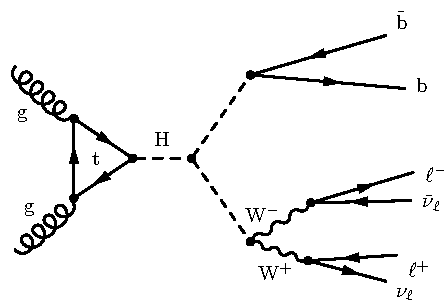
\includegraphics[bb=0 0 214 147]{figures/hh_triangle.pdf}}} &
\qquad + &
\raisebox{-.45\height}{\resizebox{0.43\textwidth}{!}{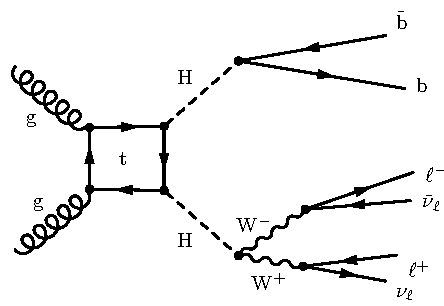
\includegraphics[bb=0 0 214 147]{figures/hh_box.pdf}}}
\end{tabular}
\end{center}
\caption{
  Leading order (LO) Feynman diagrams for the $\ggHH$ production process in $\Pp\Pp$ collisions at the LHC,
  with subsequent decay of the $\PHiggs$ boson pair via $\PHiggs\PHiggs \to \Pbottom\APbottom\PW\PW\virt \to \Pbottom\APbottom \, \ellPlusnu\ellMinusnu$.
  The asterisk ($\virt$) denotes an off-shell $\PW$ boson.
}
\label{fig:ggHH_FeynmanDiagram}
\end{figure}

The $\dihiggs$ production rate may be enhanced significantly in case an as yet unknown resonance decays to pairs of $\PHiggs$ bosons.
Such resonances are predicted in models with two Higgs doublets~\cite{Craig:2013hca,Nhung:2013lpa}, composite $\PHiggs$ boson models~\cite{Grober:2010yv,Contino:2010mh}, 
Higgs portal models~\cite{Englert:2011yb,No:2013wsa}, and models involving extra dimensions~\cite{Randall:1999ee}.
In the absence of new resonances decaying into $\PHiggs$ boson pairs,
the $\dihiggs$ production cross section may be enhanced by deviations of the couplings $\lambdaHHH$ and $\yt$ from the SM expectation for these couplings
and by the contribution of new particles to the loops 
that are present in the triangle and box diagrams shown in Fig.~\ref{fig:ggHH_FeynmanDiagram}.
%The effect of contributions from new particles to these loops can adequately be described by anomalous $\PHiggs$ boson couplings.
%More specifically,
%the production of $\PHiggs$ boson pairs via gluon fusion in Beyond the Standard Model (BSM) theories can be described to leading approximation by the non-linear Lagrangian~\cite{Buchmuller:1985jz}:
%\begin{eqnarray}
%\mathcal{L} & = & \frac{1}{2} \partial_{\mu}\PHiggs\partial^{\mu}\PHiggs - \frac{1}{2} m_{\PHiggs}^{2} \PHiggs^{2} - \kappa_{\lambda} \lambdaHHH^{\textrm{SM}} v \PHiggs^{3} \nonumber \\
% & & \quad -\frac{m_{\Ptop}}{v} \, \left( v + \kappa_{\Ptop} \PHiggs + \frac{c_{2}}{v} \PHiggs\PHiggs \right) \, \left( \bar{\Ptop}_{\textrm{L}} \Ptop_{\textrm{R}} + \textrm{h.c.} \right) 
%+ \frac{1}{4} \frac{\alpha_{\textrm{s}}}{3 \pi v} \, \left( c_{\Pgluon} \PHiggs - \frac{c_{2\Pgluon}}{2 v} \PHiggs\PHiggs \right) \, \textrm{G}^{\mu\nu}\textrm{G}_{\mu\nu} \, ,
%\end{eqnarray}
%where $v = 246$~\GeV denotes the vacuum expectation value of the Higgs field
%and the parameters $\kappa_{\lambda} = \lambdaHHH/\lambdaHHH^{\textrm{SM}}$ and $\kappa_{\Ptop} = \yt/\yt^{\textrm{SM}}$ 
%quantify the deviations of the trilinear $\PHiggs$ boson self-coupling and of the coupling of the $\PHiggs$ boson to the top quark from their SM values.
%Besides the two parameters $\kappa_{\lambda}$ and $\kappa_{\Ptop}$,
%the Lagrangian contains the coefficients of three BSM operators which account for contact interactions 
%between a $\PHiggs$ boson and either one ($c_{\Pgluon}$) or two ($c_{2\Pgluon}$) gluons
%and between a pair of $\PHiggs$ bosons and a pair of top quarks ($c_{2}$).
%The contact interactions can be interpreted in an effective field theory (EFT) approach~\cite{Buchalla:2015wfa, Goertz:2014qta}.
The effect of contributions from new particles to these loops can adequately be described by anomalous $\PHiggs$ boson couplings
in an effective field theory (EFT) approach~\cite{Buchalla:2015wfa, Goertz:2014qta}.
The production of $\PHiggs$ boson pairs in the absence of new resonances is referred to as non-resonant $\dihiggs$ production,
the case that we focus on in this paper.

%The distribution in mass of the $\PHiggs$ boson pair, $m_{\dihiggs}$, is rather broad in this case.
%Deviations of the $\PHiggs$ boson couplings from their SM values
%induces different interference patterns between the triangle and box diagrams.
%Besides affecting the $\dihiggs$ production cross section,
%the change in interference patterns may  significantly alter the distribution in $m_{\dihiggs}$
%and the distributions in the momenta and angles of the particles reconstructed in the final state.

The ATLAS and CMS collaborations have searched for non-resonant $\dihiggs$ production in the decay channels 
$\dihiggs \to \Pbottom\APbottom\Pbottom\APbottom$, $\Pbottom\APbottom\Pgt\Pgt$, $\Pbottom\APbottom\PW\PW\virt$, $\Pbottom\APbottom\Pgamma\Pgamma$
using the data recorded during LHC Runs $1$ and $2$~\cite{HIG-13-032,HIG-15-013,HIG-17-006,HIG-17-030,Sirunyan:2020xok,Aad:2015xja,Aaboud:2018knk,Aaboud:2018ftw,Aaboud:2018sfw,Aaboud:2018zhh}.
ATLAS has further performed searches in the decay channels $\dihiggs \to \Pgamma\Pgamma\PW\PW\virt$ and $\PW\PW\virt\PW\PW\virt$~\cite{Aad:2015xja,Aaboud:2018ewm,Aaboud:2018ksn}.
The asterisk ($\virt$) denotes $\PW$ bosons that are off-shell.
Phenomenological studies of non-resonant $\dihiggs$ production are presented in 
Refs.~\cite{Baur:2002rb,Baur:2002qd,Baur:2003gpa,Baur:2003gp,Dolan:2012rv,Papaefstathiou:2012qe,Baglio:2012np,deLima:2014dta,Wardrope:2014kya,Behr:2015oqq,Li:2015yia,Adhikary:2017jtu}.
No evidence for a signal has been found in the LHC data so far.
The present analyses are able to probe the existence of a SM-like $\dihiggs$ signal produced with a cross section of order $10$ times the SM production rate.

The decay channel providing the highest sensitivity for an SM-like $\dihiggs$ signal 
is the $\Pbottom\APbottom\Pgt\Pgt$ channel in case of ATLAS~\cite{Aaboud:2018sfw} and the $\Pbottom\APbottom\Pgamma\Pgamma$ channel in case of CMS~\cite{Sirunyan:2020xok}.
Both channels provide a favorable signal-to-background ratio and are limited mainly by statistical uncertainties at present,
resulting from the limited amount of data that has been recorded so far compared to the small SM $\ggHH$ production cross section.
The channels $\Pbottom\APbottom\Pbottom\APbottom$ and $\Pbottom\APbottom\PW\PW\virt$ provide a significantly larger signal rate,
but suffer from sizeable backgrounds,
arising from QCD multijet production in case of the $\Pbottom\APbottom\Pbottom\APbottom$ channel 
and from top quark pair ($\ttbar$) production in case of the $\Pbottom\APbottom\PW\PW\virt$ channel.
In this paper, we focus on the $\Pbottom\APbottom\PW\PW\virt$ channel,
and in particular on events in which both $\PW$ bosons decay to charged leptons (electrons or muons).
The latter are denoted by the symbol $\Plepton$.
 
\begin{figure}
\setlength{\unitlength}{1mm}
\begin{center}
\begin{tabular}{ccc}
\raisebox{-.45\height}{\resizebox{0.4\textwidth}{!}{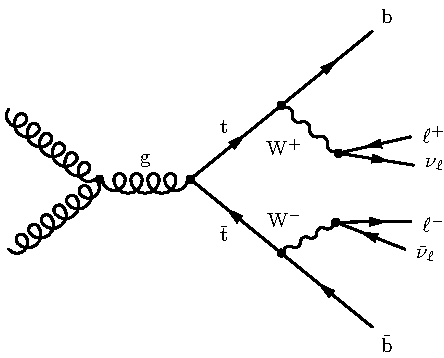
\includegraphics[bb=0 0 214 172]{figures/ttbar_tri.pdf}}} &
\qquad + &
\raisebox{-.45\height}{\resizebox{0.4\textwidth}{!}{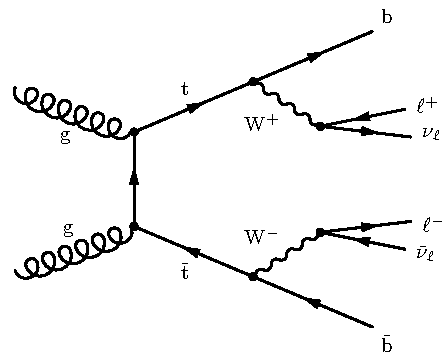
\includegraphics[bb=0 0 214 172]{figures/ttbar.pdf}}}
\end{tabular}
\end{center}
\caption{
  LO Feynman diagrams for $\ttbar$ production in $\Pp\Pp$ collisions at the LHC,
  with subsequent decay of the top quark pair via $\ttbar \to \Pbottom\PW\APbottom\PW \to \Pbottom\ellPlusnu \, \APbottom\ellMinusnu$.
}
\label{fig:ttbar_FeynmanDiagram}
\end{figure}

The separation of the $\dihiggs$ signal from the large $\ttbar$ background constitutes the main experimental challenge in the $\Pbottom\APbottom\PW\PW\virt$ channel.
For a top quark mass of $m_{\Ptop} = 172.8$~\GeV~\cite{PDG},
the cross section for $\ttbar$ production amounts to $825.9^{+46.1}_{-50.5}$~\pb at $\sqrt{s} = 13$~\TeV center-of-mass energy~\cite{Czakon:2011xx}.
The $\ttbar$ background is irreducible in this channel, as it produces the exact same multiplicity of charged leptons, neutrinos, and $\Pbottom$-jets as the $\dihiggs$ signal.
The LO Feynman diagrams for $\ttbar$ production are shown in Fig.~\ref{fig:ttbar_FeynmanDiagram}.
The main handle to separate the $\dihiggs$ signal from the $\ttbar$ background is the difference in event kinematics,
that is, the differences in the distributions of energies and angles of the charged leptons, $\Pbottom$-jets, and of the missing transverse momentum reconstructed in the event.

The present CMS analysis~\cite{HIG-17-006} utilizes machine-learning methods, based on a Deep Neural Network~\cite{ANN,chollet2015keras},
to separate the $\dihiggs$ signal from the $\ttbar$ background, while the current ATLAS analysis~\cite{Aaboud:2018zhh} employs a sequence of hard cuts for this purpose.
In this paper, we propose an alternative multivariate method for the separation of the $\dihiggs$ signal from the $\ttbar$ background,
the matrix element method (MEM)~\cite{Kondo:1988yd,Kondo:1991dw}.

The paper is structured as follows:
In Section~\ref{sec:mem} we describe the MEM and its application to the $\Pbottom\APbottom\PW\PW\virt$ channel.
The application of the MEM requires the computation of multi-dimensional integrals.
The integration is performed numerically and demands a significant amount of computing time, in the order of a few seconds per event.
In order to make the integrals suitable for numeric integration, analytic transformations need to be performed.
The most relevant of these transformations will be described in Section~\ref{sec:mem} and further details will be given in the appendix.
The performance of the MEM in separating the $\dihiggs$ signal from the $\ttbar$ background is studied in Section~\ref{sec:performance}.
The separation is studied on Monte-Carlo truth and on detector level,
for experimental conditions that are characteristic for the ATLAS and CMS experiments during LHC Run $2$.
The latter are simulated using the $\textsc{DELPHES}$ fast-simulation package~\cite{deFavereau:2013fsa}.
%We also study the effect of using matrix elements of leading order when applying the MEM to the $\Pbottom\APbottom\PW\PW\virt$ channel
%and estimate the computing time required by the method.
We conclude the paper with a summary in Section~\ref{sec:summary}.

\section{The Matrix element method}
\label{sec:mem}

The MEM computes probability densities (PDs) $w_{i}(\vecy)$
for obtaining the measured observables $\vecy$, assuming that the event has been produced by the process $i$.
The PDs $w_{i}(\vecy)$ are interpreted as quantifying the compatibility of the measured observables $\vecy$
with the signal ($i=0$) and background ($i=1$) hypothesis.
In the analysis of $\PHiggs\PHiggs$ production in the decay channel 
$\PHiggs\PHiggs \to \Pbottom\APbottom\PW\PW^{\ast} \to \Pbottom\APbottom \, \ellPlusnu\ellMinusnu$
the observables $\vecy$ refer to 
the measured momenta of the two $\Pbottom$-jets, of the two charged leptons, and of the measured missing transverse momentum ($\vecMET$) in the event.
The vector $\vecMET$ represents the measured value of the vectorial sum of the two neutrino momenta in the plane transverse to the beam axis.
We use symbols with a hat to denote the true values of energies and momenta.
Bold letters denote vector quantities.
The vector $\vecyhat$ denotes the true values of the $\Pbottom$-jet and charged lepton momenta and the true values of the momenta of the two neutrinos produced in the $\PW$ boson decays.

As already mentioned, $\PHiggs\PHiggs \to \Pbottom\APbottom\PW\PW^{\ast} \to \Pbottom\APbottom \, \ellPlusnu\ellMinusnu$ signal events
contain the same number of $\Pbottom$-jets, charged leptons, and neutrinos as the dominant background,
arising from $\ttbar \to \Pbottom\PW\APbottom\PW \to \Pbottom\ellPlusnu \, \APbottom\ellMinusnu$.
The separation of the $\PHiggs\PHiggs$ signal from the irreducible $\ttbar$ background is based on the difference in event kinematics,
causing the PD $w_{0}(\vecy)$ to be in general higher when evaluated on signal events
and lower when evaluated on background events, and vice versa for the PD $w_{1}(\vecy)$.
Given the PDs $w_{0}(\vecy)$ and $w_{1}(\vecy)$ for the signal and background hypotheses,
the Neyman-Pearson lemma~\cite{Neyman:1937uhy} postulates that the likelihood ratio (LR):
\begin{linenowrapper}
\begin{equation}
P(\vecy) = \frac{w_{0}(\vecy)}{w_{0}(\vecy) + w_{1}(\vecy)}
\label{eq:memLR}
\end{equation}
\end{linenowrapper}
provides the optimal separation of the $\PHiggs\PHiggs$ signal from the irreducible $\ttbar$ background.

Different nomenclatures and conventions for the MEM exist in the literature.
In this note, we follow the nomenclature and conventions introduced in Ref.~\cite{Volobouev:2011vb}.
The PDs $w_{i}(\vecy)$ are given by the integral:
\begin{linenowrapper}
\begin{align}
w_{i}(\vecy) = & \frac{\Omega(\vecy)}{\sigma_{i} \cdot \mathcal{A}_{i}} \, \int \, d\xhat_{a} \, d\xhat_{b} \,
  d\Phi_{n} \, \frac{f(\xhat_{a}) \, f(\xhat_{b})}{2 \, \xhat_{a} \, \xhat_{b} \, s} \, (2\pi)^{4} \,
  \delta\left( \xhat_{a} \, \Ehat_{a} + \xhat_{b} \, \Ehat_{b} - \sum_{k}^{n} \Ehat_{(k)} \right) \nonumber \\
 & \quad \cdot \, \delta^{3}\left( \xhat_{a} \, \vecphat^{a} + \xhat_{b} \, \vecphat^{b} - \sum_{k}^{n} \vecphat^{(k)}\right) \, 
  \vert \mathcal{M}_{i}(\vecyhat) \vert^{2} \, W(\vecy|\vecyhat) \, \epsilon_{i}(\vecyhat) \, .
\label{eq:mem1}
\end{align}
\end{linenowrapper}
The symbol $\vert \mathcal{M}_{i}(\vecyhat) \vert^{2}$ denotes the squared modulus of the matrix element (ME),
averaged over helicity states,
for either the signal ($i=0$) or for the background ($i=1$) hypothesis.
We use ME generated at LO accuracy with the program MadGraph\_aMCatNLO 2.3.3~\cite{MadGraph_aMCatNLO} for the signal as well as for the background hypothesis.
Our choice of using LO ME is motivated by the observation that using ME generated at NLO accuracy in pQCD
would increase the computing-time requirements of the MEM by one to two orders of magnitude. 
As we will discuss in more detail in Section~\ref{sec:computing_time_requirements}, the demand in computing time is challenging already when using ME generated at LO accuracy.

The symbols $\Ehat_{a}$ and $\Ehat_{b}$ ($\vecphat^{a}$ and $\vecphat^{b}$) denote the energies (momenta) of the two colliding protons,
$\sqrt{s}$ their center-of-mass energy,
$\xhat_{a}$ and $\xhat_{b}$ the Bjorken scaling variables~\cite{Bjorkenx},
and $f(\xhat_{a})$ and $f(\xhat_{b})$ the corresponding parton distribution functions (PDFs).
We use the MSTW 2008 LO PDF set~\cite{MSTW} to evaluate $f(\xhat_{a})$ and $f(\xhat_{b})$.
We denote by $n$ the number of particles in the final state,
and by $\vecp^{(k)}$ ($\vecphat^{(k)}$) the measured (true) momentum of the $k$-th final state particle. 
The $\delta$-functions $\delta( \xhat_{a} \, \Ehat_{a} + \xhat_{b} \, \Ehat_{b} - \sum_{k}^{n} \Ehat_{(k)})$
and $\delta^{3}( \xhat_{a} \, \vecphat^{a} + \xhat_{b} \, \vecphat^{b} - \sum_{k}^{n} \vecphat^{(k)})$ 
impose conservation of energy and momentum.

The functions $W(\vecy|\vecyhat)$ are referred to as ``transfer functions'' (TF) in the literature.
They represent the PD to observe the measured values $\vecy$, given the true values $\vecyhat$.
The function $\Omega(\vecy)$ is referred to as ``indicator function'' in the literature~\cite{Fiedler:2010sg,Volobouev:2011vb}.
It attains the value $1$ in case the event represented by the measured observables $\vecy$ passes the event selection criteria and otherwise attains the value $0$.
The efficiency for an event originating at the phase-space (PS) point
$\vecyhat$ to pass the event selection, \ie to end up with measured
observables $\vecy$ for which $\Omega(\vecy) = 1$,
is denoted by $\epsilon_{i}(\vecyhat)$. 
Finally, the symbol $\mathcal{A}_{i}$ denotes the acceptance of the event selection, 
that is, the percentage of events which pass the event selection criteria,
while $\sigma_{i}$ denotes the cross section of process $i$.
The subscript $i$ of the symbols $\sigma_{i}$, $\mathcal{A}_{i}$, and $\epsilon_{i}$ 
emphasize that the cross section, acceptance, and efficiency differ between the signal and the background hypothesis.
Division of the right-hand-side (RHS) of Eq.~(\ref{eq:mem1}) by the product $\sigma_{i} \cdot \mathcal{A}_{i}$
ensures that $w_{i}(\vecy)$ has the correct normalization required for a probability density, 
\ie $\int \, d\vecy \, w_{i}(\vecy) = 1$,
provided that the TF satisfy the normalization condition
$\int \, d\vecy \, \Omega(\vecy) \, W(\vecy|\vecyhat) = 1$
for every $\vecy$.

The symbol $d\Phi_{n} = \prod_{k}^{n} \, \frac{d^{3}\vecphat^{(k)}}{(2\pi)^{3} \, 2 \Ehat_{(k)}}$ 
represents the differential $n$-particle PS element.
For the $\PHiggs\PHiggs$ signal 
as well as for the $\ttbar$ background hypothesis, $n=6$.  
We express the PS element $d\Phi_{6}$ in terms of the energies $\Ehat_{(k)}$, the polar angles $\thetahat_{(k)}$, and the azimuthal angles $\phihat_{(k)}$ 
of the two $\Pbottom$ quarks, of the two charged leptons, and of the two neutrinos:
\begin{linenowrapper}
\begin{eqnarray}
d\Phi_{6} 
 & = &\prod_{k}^{6} \, \frac{d^{3}\vecphat^{(k)}}{(2 \, \pi)^{3} \, 2 \, \Ehat_{(k)}} 
  = \frac{1}{2^{24} \, \pi^{18}} \, \prod_{k}^{6} \, 
\frac{d^{3}\vecphat^{(k)}}{\Ehat_{(k)}} \nonumber \\
 & = & \frac{1}{2^{24} \, \pi^{18}} \, \prod_{k}^{6} \, 
\frac{d\Ehat_{(k)} \, d\thetahat_{(k)} \, d\phihat_{(k)} \, |\vecphat^{(k)}| \, \Ehat_{(k)} \, \sin\thetahat_{(k)}}{\Ehat_{(k)}} \nonumber \\
 & = & \frac{1}{2^{24} \, \pi^{18}} \, \prod_{k}^{6} \, 
d\Ehat_{(k)} \, d\thetahat_{(k)} \, d\phihat_{(k)} \, \betahat_{(k)} \Ehat_{(k)} \, \sin\thetahat_{(k)} \, .
\label{eq:PS_inPolarCoordinates}
\end{eqnarray}
\end{linenowrapper}
All energies $\Ehat_{(k)}$ as well as the angles $\thetahat_{(k)}$ and $\phihat_{(k)}$ refer to the laboratory (detector) frame.
The velocity $\betahat_{(k)}$ of particle $k$,
given by $\betahat_{(k)} \equiv \frac{|\vecphat^{(k)}|}{\Ehat_{(k)}}$,
has been used to simplify the expression for $d\Phi_{6}$ in the last step.
Note that the velocity $\betahat_{(k)}$ is a function of energy $\Ehat_{(k)}$ and hence cannot be treated as constant when evaluating the integral over $d\Ehat_{(k)}$.
Similarly, the magnitude of the momentum $|\vecphat^{(k)}|$ is a function of the energy $\Ehat_{(k)}$.
In the following, we use the identities $|\vecphat^{(k)}| = \sqrt{\Ehat_{(k)}^{2} - m_{(k)}^{2}}$ 
and $\betahat_{(k)} = \frac{\sqrt{\Ehat_{(k)}^{2} - m_{(k)}^{2}}}{\Ehat_{(k)}}$ to make the dependency on the energy $\Ehat_{(k)}$ explicit.

The form of Eq.~(\ref{eq:PS_inPolarCoordinates}) is useful, 
as it allows to trivially perform the integration over the 
angles $\thetahat_{(k)}$ and $\phihat_{(k)}$ for the two $\Pbottom$ quarks and for the two charged leptons,
taking advantage of the fact that the directions of quarks (jets) and charged leptons can be measured with negligible experimental resolution.
With the further assumption that also the energy of charged leptons can be measured with negligible experimental resolution,
the integration over $d\Ehat_{\Plepton^{+}}$ and $d\Ehat_{\Plepton^{-}}$ can be carried out trivially too.
We shall only consider events that pass the event selection criteria, \ie for which the indicator function $\Omega(\vecy)$ is equal to $1$.
For simplicity, we neglect the effect of the efficiency $\epsilon_{i}(\vecyhat)$ and of the acceptance $\mathcal{A}_{i}$.
With these assumptions and upon inserting the expressions for the TF given by Eqs.~(\ref{eq:TF_ell}),~(\ref{eq:TF_b}), and~(\ref{eq:TF_f}) in the appendix
into Eq.~(\ref{eq:PS_inPolarCoordinates}), we obtain:
\begin{linenowrapper}
\begin{align}
w_{i}(\vecy) 
 = & \frac{1}{2^{24} \, \pi^{18} \, \sigma_{i} \, E_{\Plepton^{+}} \, E_{\Plepton^{-}}} \, \int \, d\xhat_{a} \, d\xhat_{b} \,
\frac{d\Ehat_{\Pbottom}}{\Ehat_{\Pbottom}} \, \frac{d\Ehat_{\APbottom}}{\Ehat_{\APbottom}} \, \frac{d^{3}\vecphat_{\Pnu}}{\Ehat_{\Pnu}} \, \frac{d^{3}\vecphat_{\APnu}}{\Ehat_{\APnu}} \,
\frac{f(\xhat_{a}) \, f(\xhat_{b})}{2 \, \xhat_{a} \, \xhat_{b} \, s} \nonumber \\
 & \quad \cdot \, (2 \, \pi)^{4} \, \delta\left( \xhat_{a} \, \Ehat_{a} + \xhat_{b} \, \Ehat_{b} - \sum_{k}^{6} \Ehat_{(k)}\right) \, 
\delta^{3}\left( \xhat_{a} \, \vecphat^{a} + \xhat_{b} \, \vecphat^{b} - \sum_{k}^{6} \vecphat^{(k)}\right) \nonumber \\
 & \quad \cdot \, \vert \mathcal{M}_{i}(\vecphat) \vert^{2} \, \frac{\betahat_{\Pbottom} \, \Ehat_{\Pbottom}^{2}}{\beta_{\Pbottom} \, E_{\Pbottom}^{2}} \, W(E_{\Pbottom}|\Ehat_{\Pbottom}) \, 
\frac{\betahat_{\APbottom} \, \Ehat_{\APbottom}^{2}}{\beta_{\APbottom} \, E_{\APbottom}^{2}} \, W(E_{\APbottom}|\Ehat_{\APbottom}) \nonumber \\
 = & \frac{1}{2^{21} \, \pi^{14} \, \sigma_{i} \, E_{\Plepton^{+}} \, E_{\Plepton^{-}} \, E_{\Pbottom} \, E_{\APbottom}} \, \int \, d\xhat_{a} \, d\xhat_{b} \,
d\Ehat_{\Pbottom} \, d\Ehat_{\APbottom} \, \frac{d^{3}\vecphat_{\Pnu}}{\Ehat_{\Pnu}} \, \frac{d^{3}\vecphat_{\APnu}}{\Ehat_{\APnu}} \,
\frac{f(\xhat_{a}) \, f(\xhat_{b})}{\xhat_{a} \, \xhat_{b} \, s} \nonumber \\
 & \quad \cdot \, \delta\left( \xhat_{a} \, \Ehat_{a} + \xhat_{b} \, \Ehat_{b} - \sum_{k}^{6} \Ehat_{(k)}\right) \,
\delta^{3}\left( \xhat_{a} \, \vecphat^{a} + \xhat_{b} \, \vecphat^{b} - \sum_{k}^{6} \vecphat^{(k)}\right) \nonumber \\
 & \quad \cdot \, \vert \mathcal{M}_{i}(\vecphat) \vert^{2}\, \frac{\betahat_{\Pbottom} \, \Ehat_{\Pbottom}}{\beta_{\Pbottom} \, E_{\Pbottom}} \, W(E_{\Pbottom}|\Ehat_{\Pbottom}) \, 
\frac{\betahat_{\APbottom} \, \Ehat_{\APbottom}}{\beta_{\APbottom} \, E_{\APbottom}} \, W(E_{\APbottom}|\Ehat_{\APbottom}) \, .
\label{eq:mem2}
\end{align}
\end{linenowrapper}
The terms $\frac{\betahat_{\Pbottom} \, \Ehat_{\Pbottom}}{\beta_{\Pbottom} \, E_{\Pbottom}}$ and $\frac{\betahat_{\APbottom} \, \Ehat_{\APbottom}}{\beta_{\APbottom} \, E_{\APbottom}}$ 
arise because the integration over the PS elements $d^{3}\vecphat$ of the $\Pbottom$ and $\APbottom$ quarks yields a factor $\betahat \, \Ehat^{2} \, \sin\thetahat$,
while the normalization of the TF yields a factor $\frac{1}{\beta \, E^{2} \, \sin\theta}$, \cf Eq.~(\ref{eq:TF_f}).
The terms $\sin\thetahat$ and $\frac{1}{\sin\theta}$ cancel, due to the presence of the $\delta$-function $\delta(\theta - \thetahat)$ in the integrand, \cf Eq.~(\ref{eq:TF_b}).
No similar terms arise for the charged leptons, as the TF for charged leptons demand $\betahat = \beta$, $\Ehat = E$, and $\thetahat = \theta$, \cf Eq.~(\ref{eq:TF_ell}).

We simplify the four-dimensional $\delta$-function 
$\delta( \xhat_{a} \, \Ehat_{a} + \xhat_{b} \, \Ehat_{b} - \sum_{k}^{6} \Ehat_{(k)}) \cdot \delta^{3}( \xhat_{a} \, \vecphat^{a} + \xhat_{b} \, \vecphat^{b} - \sum_{k}^{6} \vecphat^{(k)})$
by assuming the momentum vectors of the colliding protons to be aligned in direction parallel and anti-parallel to the beam axis 
and neglecting the small transverse momenta of the partons within the protons as well as parton masses.
With this assumption, we can eliminate the energy and longitudinal momentum components of the $\delta$-function 
and solve for the Bjorken scaling variables $\xhat_{a}$ and $\xhat_{b}$ as function of the energies and longitudinal momenta of the particles in the final state.
This yields:
\begin{linenowrapper}
\begin{equation}
\xhat_{a} = \frac{1}{\sqrt{s}} \, \sum_{k}^{6} \Ehat_{(k)} + \pZhat^{(k)} \quad \mbox{ and } \quad
\xhat_{b} = \frac{1}{\sqrt{s}} \, \sum_{k}^{6} \Ehat_{(k)} - \pZhat^{(k)} \, .
\label{eq:Bjorkenx}
\end{equation}
\end{linenowrapper}

For the purpose of eliminating the transverse momentum components of the four-dimensional $\delta$-function,
we follow the approach of Ref.~\cite{SVfitMEM}.
The approach is based on introducing the ``hadronic recoil'', denoted by the symbol $\rho$, as a means to account for QCD radiation,
which causes additional jets to be produced besides the two $\Pbottom$-jets originating from the decay of the $\PHiggs$ boson (in signal events) 
or from the decay of the two top quarks (in background events).
As detailed in Ref.~\cite{Alwall:2010cq}, significant amounts of QCD radiation, in particular initial-state radiation (ISR),
are a typical feature of most signal and background processes at the LHC.
The longitudinal momentum of the additional jets produced by QCD radiation alters the relations for $\xhat_{a}$ and $\xhat_{b}$ somewhat,
compared to the values given by Eq.~(\ref{eq:Bjorkenx}).
We expect the effect of QCD radiation on the energy and longitudinal momentum components to be small and thus neglect it.
The effect on the transverse momentum balance is important, however,
as QCD radiation distorts the kinematic relations that would be expected to hold in the absence of such radiation.
As a consequence, the $\delta$-functions that ensure the conservation of momentum in the transverse plane need to be modified. 
Their modified form reads: 
$\delta( \pXhat^{\rho} + \sum_{k}^{6} \pXhat^{(k)})$ and $\delta( \pYhat^{\rho} + \sum_{k}^{6} \pYhat^{(k)})$,
where $\pXhat^{\rho}$ and $\pYhat^{\rho}$ denote the true value of the momentum of the hadronic recoil $\rho$ in $x$ and $y$ direction, respectively.
They imply the relations:
\begin{linenowrapper}
\begin{equation}
\pXhat^{\rho} = - \left( \pXhat^{\Pbottom} + \pXhat^{\APbottom} + \pXhat^{\Plepton^{+}} + \pXhat^{\Pnu} + \pXhat^{\Plepton^{-}} + \pXhat^{\APnu} \right) \, \mbox{ and } \,
\pYhat^{\rho} = - \left( \pYhat^{\Pbottom} + \pYhat^{\APbottom} + \pYhat^{\Plepton^{+}} + \pYhat^{\Pnu} + \pYhat^{\Plepton^{-}} + \pYhat^{\APnu} \right) \, .
\label{eq:hadRecoil_true}
\end{equation}
\end{linenowrapper}
The corresponding relations for the measured momenta read:
\begin{linenowrapper}
\begin{equation}
\pX^{\rho} = - \left( \pX^{\Pbottom} + \pX^{\APbottom} + \pX^{\Plepton^{+}} + \pX^{\Plepton^{-}} + \METx \right) \, \mbox{ and } \,
\pY^{\rho} = - \left( \pY^{\Pbottom} + \pY^{\APbottom} + \pY^{\Plepton^{+}} + \pY^{\Plepton^{-}} + \METy \right) \, .
\label{eq:hadRecoil}
\end{equation}
\end{linenowrapper}
We use Eq.~(\ref{eq:hadRecoil}) to compute the measured values of $\pX^{\rho}$ and $\pY^{\rho}$, 
given the measured momenta of the two $\Pbottom$-jets, of the two charged leptons, and of the measured $\vecMET$.
The experimental resolution on $\pX^{\rho}$ and $\pY^{\rho}$ is accounted for by introducing a TF for the hadronic recoil into the integrand of Eq.~(\ref{eq:mem2}).
We assume that the resolution on the transverse momentum components of $\rho$ follows a two-dimensional normal distribution:
\begin{linenowrapper}
\begin{equation}
W_{\rho}( \pX^{\rho},\pY^{\rho} | \pXhat^{\rho},\pYhat^{\rho} ) = 
 \frac{1}{2\pi \, \sqrt{\vert V \vert}} \, \exp \left( -\frac{1}{2}
 \left( \begin{array}{c} \pX^{\rho} - \pXhat^{\rho} \\ \pY^{\rho} - \pYhat^{\rho} \end{array} \right)^{T}
  \cdot V^{-1} \cdot
   \left( \begin{array}{c} \pX^{\rho} - \pXhat^{\rho} \\ \pY^{\rho} - \pYhat^{\rho} \end{array} \right)
 \right) \, ,
\label{eq:TF_hadRecoil}
\end{equation}
\end{linenowrapper}
where the matrix $V$ quantifies the resolution on the hadronic recoil in the transverse plane.

The CMS collaboration computes the matrix $V$ on an event-by-event basis, using an algorithm referred to as the ``$\MET$-significance'' algorithm~\cite{JME-10-009}.
Alternatively, one could determine an average resolution $\sigma_{\rho}$ for a sample of $\dihiggs$ signal and $\ttbar$ background events using the Monte Carlo simulation
and take the matrix $V$ to be $V = \sigma_{\rho}^{2} \cdot I_{2}$, where $I_{2}$ denotes the identity matrix of size $2$.
We follow the procedure detailed in Ref.~\cite{SVfitMEM} and replace the $\delta$-functions 
$\delta( \pXhat^{\rho} + \sum_{k}^{6} \pXhat^{(k)})$ and $\delta( \pYhat^{\rho} + \sum_{k}^{6} \pYhat^{(k)})$,
which ensure the momentum conservation in the transverse plane,
with the TF for the hadronic recoil, given by Eq.~(\ref{eq:TF_hadRecoil}).

A remaining issue is that we use LO ME $\mathcal{M}_{i}(\vecphat)$ for the $\PHiggs\PHiggs$ signal and for the $\ttbar$ background in Eq.~(\ref{eq:mem2}).
The LO ME for the signal (background) requires that the $\PHiggs\PHiggs$ ($\ttbar$) system has zero $\pT$, 
a condition that only holds in case the hadronic recoil has zero $\pT$.
As previously discussed, the case that the hadronic recoil has negligible $\pT$ is rare at the LHC, due to the abundance of QCD radiation.
The issue that the LO ME is only well-defined for events with zero ISR
is resolved by evaluating the ME $\mathcal{M}_{i}(\vecyhat)$ in a frame in which the $\PHiggs\PHiggs$ ($\ttbar$) system has zero $\pT$, 
to which we refer as the zero-transverse-momentum (ZTM) frame.
The Lorentz transformation of the energy $\Ehat_{(k)}$ and momenta $\vecphat^{(k)}$ in Eq.~(\ref{eq:mem2})
from the laboratory to the ZTM frame is performed using the vector $\left(-\frac{\pX^{\rho}}{\pT^{\rho}},-\frac{\pY^{\rho}}{\pT^{\rho}},0\right)$ as the boost vector.

Eliminating the energy and longitudinal momentum components of the four-dimensional $\delta$-function 
$\delta( \xhat_{a} \, \Ehat_{a} + \xhat_{b} \, \Ehat_{b} - \sum_{k}^{6} \Ehat_{(k)}) \cdot \delta( \xhat_{a} \, \pZhat^{a} + \xhat_{b} \, \pZhat^{b} - \sum_{k}^{6} \pZhat^{(k)}) \cdot \delta( \pXhat^{\rho} + \sum_{k}^{6} \pXhat^{(k)}) \cdot \delta( \pYhat^{\rho} + \sum_{k}^{6} \pYhat^{(k)})$
by means of Eq.~(\ref{eq:Bjorkenx})
and replacing its transverse momentum components by the TF $W_{\rho}( \pX^{\rho},\pY^{\rho} | \pXhat^{\rho},\pYhat^{\rho} )$ for the hadronic recoil $\rho$,
the expression for the PD $w_{i}(\vecy)$ becomes:
\begin{linenowrapper}
\begin{align}
w_{i}(\vecy) 
 = & \frac{1}{2^{21} \, \pi^{14} \, \sigma_{i} \, E_{\Plepton^{+}} \, E_{\Plepton^{-}} \, E_{\Pbottom} \, E_{\APbottom}} \, \int \, 
d\Ehat_{\Pbottom} \, d\Ehat_{\APbottom} \, \frac{d^{3}\vecphat_{\Pnu}}{\Ehat_{\Pnu}} \, \frac{d^{3}\vecphat_{\APnu}}{\Ehat_{\APnu}} \,
\frac{f(\xhat_{a}) \, f(\xhat_{b})}{\xhat_{a} \, \xhat_{b} \, s} \nonumber \\
 & \quad \cdot \, \vert \mathcal{M}_{i}(\vecphat) \vert^{2} \, 
\frac{\betahat_{\Pbottom} \, \Ehat_{\Pbottom}}{\beta_{\Pbottom} \, E_{\Pbottom}} \, W(E_{\Pbottom}|\Ehat_{\Pbottom}) \, 
\frac{\betahat_{\APbottom} \, \Ehat_{\APbottom}}{\beta_{\APbottom} \, E_{\APbottom}} \, W(E_{\APbottom}|\Ehat_{\APbottom}) \, W_{\rho}( \pX^{\rho},\pY^{\rho} | \pXhat^{\rho},\pYhat^{\rho} ) \nonumber \\
 = & \frac{1}{2^{21} \, \pi^{14} \, \sigma_{i} \, E_{\Plepton^{+}} \, E_{\Plepton^{-}} \, E_{\Pbottom} \, E_{\APbottom}} \, \int \, 
d\Ehat_{\Pbottom} \, d\Ehat_{\APbottom} \, d\Ehat_{\Pnu} \, d\thetahat_{\Pnu} \, d\phihat_{\Pnu} \, d\Ehat_{\APnu} \, d\thetahat_{\APnu} \, d\phihat_{\APnu} \nonumber \\
 & \quad \cdot \, \betahat_{\Pnu} \, \Ehat_{\Pnu} \, \sin\thetahat_{\Pnu} \, 
\betahat_{\APnu} \, \Ehat_{\APnu} \, \sin\thetahat_{\APnu} \, 
\frac{f(\xhat_{a}) \, f(\xhat_{b})}{\xhat_{a} \, \xhat_{b} \, s} \nonumber \\
 & \quad \cdot \, \vert \mathcal{M}_{i}(\vecphat) \vert^{2} \, 
\frac{\betahat_{\Pbottom} \, \Ehat_{\Pbottom}}{\beta_{\Pbottom} \, E_{\Pbottom}} \, W(E_{\Pbottom}|\Ehat_{\Pbottom}) \, 
\frac{\betahat_{\APbottom} \, \Ehat_{\APbottom}}{\beta_{\APbottom} \, E_{\APbottom}} \, W(E_{\APbottom}|\Ehat_{\APbottom}) \, W_{\rho}( \pX^{\rho},\pY^{\rho} | \pXhat^{\rho},\pYhat^{\rho} ) \, .
\label{eq:mem3}
\end{align}
\end{linenowrapper}
The expression in Eq.~(\ref{eq:mem3}) concludes our discussion of analytic transformations of the expressions for the PD $w_{i}(\vecy)$ 
that are common to the signal as well as to the background hypothesis.
A few more analytic transformations need to be performed to handle the presence of Breit-Wigner (BW) propagators in the ME $\mathcal{M}_{i}(\vecphat)$,
as the presence of these propagators represent an obstacle for the numeric integration of Eq.~(\ref{eq:mem3}).
The effect of the BW propagators is that only narrow slices in the $6$-particle PS yield sizeable contribution to the integral,
namely the regions where the $6$ final state particles satisfy certain mass constraints.
The mass constraints arise from the presence of on-shell $\PHiggs$ bosons, $\PW$ bosons, and top quarks in the decay chains
$\PHiggs\PHiggs \to \Pbottom\APbottom\PW\PW^{\ast} \to \Pbottom\APbottom \, \ellPlusnu\ellMinusnu$ and
$\ttbar \to \Pbottom\PW\APbottom\PW \to \Pbottom\ellPlusnu \, \APbottom\ellMinusnu$.
Their presence renders the numeric integration inefficient, unless the mass constraints are treated analytically. 
We use the narrow-width approximation (NWA)~\cite{NWA} to handle the mass constraints and replace the BW propagators by $\delta$-functions.
The NWA has the effect of restricting the numerical integration to the narrow slices in the $6$-particle PS where the mass constraints are satisfied
and the ME $\mathcal{M}_{i}(\vecphat)$ yields a sizeable contribution to the integral.
The analytic transformations that are needed to handle the BW propagators differ for the signal and for the background hypothesis,
reflecting the presence of different resonances in the respective decay chains.
The transformations that are specific to the signal hypothesis are detailed in Section~\ref{sec:mem_signal},
while those specific to the background hypothesis are presented in Section~\ref{sec:mem_background}.

Finally, the numeric integration is performed using the VAMP algorithm~\cite{VAMP}, a variant of the popular VEGAS algorithm~\cite{VEGAS},
which has been optimized for the case of integrating multimodal functions, typically appearing in the integration of ME over regions in PS.
We use $2500$ evaluations of the integrand when computing the PD $w_{0}(\vecy)$ for the signal hypothesis 
and $25000$ evaluations of the integrand for the computation of the PD $w_{1}(\vecy)$ for the background hypothesis.
The number of evaluations has been chosen such that the computation of $w_{0}(\vecy)$ and $w_{1}(\vecy)$ take approximately the same time
and the computation of the likelihood ratio $P(\vecy)$ takes about one minute per event,
using a single core of a $2.30$~GHz Intel\TReg~Xeon\TReg~E5-2695V3 processor.


\subsection{Analytic transformations specific to the signal hypothesis}
\label{sec:mem_signal}

When evaluating the integrand in Eq.~(\ref{eq:mem3}) for the signal hypothesis,
only those points in the $6$-particle PS provide a sizeable contribution to the value of the integral $w_{0}(\vecy)$
which satisfy the following conditions:
\begin{itemize}
\item The mass of the $2$-particle system comprised of the two $\Pbottom$ quarks equals $m_{\PHiggs} = 125.1$~\GeV~\cite{HIG-14-042}.
\item The mass of the $2$-particle system comprised of the charged lepton and of the neutrino, which originate from the decay of the on-shell $\PW$ boson, equals $m_{\PW} = 80.4$~\GeV~\cite{PDG}.
\item The mass of the $4$-particle system comprised of the two charged leptons and of the two neutrinos equals $m_{\PHiggs}$.
\end{itemize}

We formally introduce these mass constraints by inserting three $\delta$-functions $\delta\left( g(x) \right)$ into the integrand of Eq.~(\ref{eq:mem3}).
The procedure is explained in Section~\ref{sec:appendix_mass_constraints} of the appendix.
More specifically, we insert
one $\delta$-function of the type $g(\Ehat_{\APbottom})$ given by Eq.~(\ref{eq:bEn_Hbb1}), 
one of the type $g(\Ehat_{\Pnu})$ given by Eq.~(\ref{eq:nuEn_Wlnu1}), and one of the type $g(\Ehat_{\nuStar})$ given by Eq.~(\ref{eq:nuEn_Hww1}) into the integrand of Eq.~(\ref{eq:mem3}).
We denote the charged lepton and the neutrino originating from the decay of the off-shell $\PW$ boson, which can be either the $\PW^{+}$ or the $\PW^{-}$, by an asterisk.
The charged lepton and the neutrino that are referred to without asterisks are subject to the $\PW$ mass constraint.

After solving for the $\delta$-functions analytically, as detailed in Sections~\ref{sec:appendix_bEn_Hbb}, ~\ref{sec:appendix_nuEn_Wlnu}, and~\ref{sec:appendix_nuEn_Hww} of the appendix,
the resulting expression for the PD $w_{0}(\vecy)$ for the signal hypothesis reads:
\begin{linenowrapper}
\begin{align}
w_{0}(\vecy) 
 = & \frac{(m_{\PHiggs} \, \Gamma_{\PHiggs})^{2} \, m_{\PW} \, \Gamma_{\PW}}{2^{21} \, \pi^{14} \, \sigma_{0} \, E_{\Plepton} \, E_{\ellStar} \, E_{\Pbottom} \, E_{\APbottom}} \, \int \,
d\Ehat_{\Pbottom} \, d\thetahat_{\Pnu} \, d\phihat_{\Pnu} \, d\thetahat_{\nuStar} \, d\phihat_{\nuStar}  \nonumber \\
 & \quad \cdot \, \underbrace{\betahat_{\Pnu}}_{= 1} \, \underbrace{\Ehat_{\Pnu} \, \sin\thetahat_{\Pnu}}_{= \pThat^{\Pnu}} \, 
  \underbrace{\betahat_{\nuStar}}_{= 1} \, \underbrace{\Ehat_{\nuStar} \, \sin\thetahat_{\nuStar}}_{= \pThat^{\nuStar}} \, 
\frac{f(\xhat_{a}) \, f(\xhat_{b})}{\xhat_{a} \, \xhat_{b} \, s} \nonumber \\
 & \quad \cdot \, \vert \mathcal{M}_{0}(\vecphat) \vert^{2} \, 
\frac{\betahat_{\Pbottom} \, \Ehat_{\Pbottom}}{\beta_{\Pbottom} \, E_{\Pbottom}} \, W(E_{\Pbottom}|\Ehat_{\Pbottom}) \, 
\frac{\betahat_{\APbottom} \, \Ehat_{\APbottom}}{\beta_{\APbottom} \, E_{\APbottom}} \, W(E_{\APbottom}|\Ehat_{\APbottom}) \,
W_{\rho}( \pX^{\rho},\pY^{\rho} | \pXhat^{\rho},\pYhat^{\rho} ) \nonumber \\
 & \quad \cdot \, \frac{1}{\Ehat_{\Pbottom} \, \left( 1 - \frac{\betahat_{\Pbottom}}{\betahat_{\APbottom}} \, \cos\sphericalangle(\vece_{\Pbottom},\vece_{\APbottom}) \right)} \nonumber \\
 & \quad \cdot \, \frac{1}{4 \, E_{\Plepton} \, \sin^{2}\left(\frac{\sphericalangle(\vece_{\Plepton},\vecehat_{\Pnu})}{2}\right)} \,
\frac{1}{\Ehat_{\ellnuellStar} \left( 1 - \betahat_{\ellnuellStar} \, \cos\sphericalangle(\vecehat_{\ellnuellStar},\vecehat_{\nuStar}) \right)} \nonumber \\
 = & \frac{(m_{\PHiggs} \, \Gamma_{\PHiggs})^{2} \, m_{\PW} \, \Gamma_{\PW}}{2^{23} \, \pi^{14} \, \sigma_{0} \, s \, 
  E_{\Plepton}^{2} \, E_{\ellStar} \, \beta_{\Pbottom} \, E_{\Pbottom}^{2} \, \beta_{\APbottom} \, E_{\APbottom}^{2}} \, \int \,
d\Ehat_{\Pbottom} \, d\thetahat_{\Pnu} \, d\phihat_{\Pnu} \, d\thetahat_{\nuStar} \, d\phihat_{\nuStar} \nonumber \\
 & \quad \cdot \, \pThat^{\Pnu} \, \pThat^{\nuStar} \, 
\frac{f(\xhat_{a}) \, f(\xhat_{b})}{\xhat_{a} \, \xhat_{b}} \nonumber \\
 & \quad \cdot \, \vert \mathcal{M}_{0}(\vecphat) \vert^{2} \, 
\betahat_{\Pbottom} \, \Ehat_{\Pbottom} \, W(E_{\Pbottom}|\Ehat_{\Pbottom}) \, 
\betahat_{\APbottom} \, \Ehat_{\APbottom} \, W(E_{\APbottom}|\Ehat_{\APbottom}) \,
W_{\rho}( \pX^{\rho},\pY^{\rho} | \pXhat^{\rho},\pYhat^{\rho} ) \nonumber \\
 & \quad \cdot \, \frac{1}{\Ehat_{\Pbottom} \, \left( 1 - \frac{\betahat_{\Pbottom}}{\betahat_{\APbottom}} \, \cos\sphericalangle(\vece_{\Pbottom},\vece_{\APbottom}) \right)} \nonumber \\
 & \quad \cdot \, \frac{1}{\sin^{2}\left(\frac{\sphericalangle(\vece_{\Plepton},\vecehat_{\Pnu})}{2}\right)} \,
\frac{1}{\Ehat_{\ellnuellStar} \left( 1 - \betahat_{\ellnuellStar} \, \cos\sphericalangle(\vecehat_{\ellnuellStar},\vecehat_{\nuStar}) \right)} \, ,
\label{eq:mem_signal}
\end{align}
\end{linenowrapper}
with:
\begin{linenowrapper}
\begin{eqnarray}
\Ehat_{\APbottom} & = & \frac{a \, \Delta_{m_{\PHiggs}} + |b| \, \sqrt{\Delta_{m_{\PHiggs}}^{2} - (a^{2} - b^{2}) \, m_{\Pbottom}^{2}}}{a^{2} - b^{2}} \nonumber \\
\Ehat_{\Pnu} & = & \frac{m_{\PW}^{2}}{4 \, \Ehat_{\Plepton} \, \sin^{2}\left(\frac{\sphericalangle(\vece_{\Plepton},\vecehat_{\Pnu})}{2}\right)} \nonumber \\
\Ehat_{\nuStar} & = & \frac{m_{\PHiggs}^{2} - m_{\ellnuellStar}^{2}}{2 \, \Ehat_{\ellnuellStar} \, 
 \left( 1 - \betahat_{\ellnuellStar} \, \cos\sphericalangle(\vecehat_{\ellnuellStar},\vecehat_{\nuStar}) \right)} \, ,
\end{eqnarray}
\end{linenowrapper}
where:
\begin{linenowrapper}
\begin{eqnarray}
\Delta_{m_{\PHiggs}} & = & \frac{m_{\PHiggs}^{2}}{2} - m_{\Pbottom}^{2} \nonumber \\
a & = & \Ehat_{\Pbottom} \nonumber \\
b & = & \underbrace{\sqrt{\Ehat_{\Pbottom}^{2} - m_{\Pbottom}^{2}}}_{= \betahat_{\Pbottom} \, \Ehat_{\Pbottom}} \, 
 \underbrace{\vece_{\Pbottom} \cdot \vece_{\APbottom}}_{= \cos\sphericalangle(\vece_{\Pbottom},\vece_{\APbottom})} \, 
= \, \betahat_{\Pbottom} \, \Ehat_{\Pbottom} \, \cos\sphericalangle(\vece_{\Pbottom},\vece_{\APbottom}) \, .
\end{eqnarray}
\end{linenowrapper}
The integral on the RHS of Eq.~(\ref{eq:mem_signal}) is ready to be evaluated by numeric integration. 
The integral extends over the $5$ variables
 $\Ehat_{\Pbottom}$, $\thetahat_{\Pnu}$, $\phihat_{\Pnu}$, $\thetahat_{\nuStar}$, and $\phihat_{\nuStar}$.
The symbol $\vecehat_{k}$ ($\vece_{k}$) refer to unit vectors in direction of (measured) particle $k$,
and the symbol $\sphericalangle(\vecehat_{k},\vecehat_{k'})$ denotes the angle between the directions of particles $k$ and $k'$.
This notation includes the case that the ``particles'' $k$ and $k'$ are systems of multiple particles,
\eg $\vecehat_{\ellnuellStar}$ denotes the direction of the momentum vector of the $3$-particle system composed of
the charged lepton and the neutrino produced in the decay of the on-shell $\PW$ boson and of the charged lepton produced in the decay of the off-shell $\PW$ boson.

There is one further aspect, which needs to be taken into account when computing the compatibility of a given event with the signal hypothesis,
and that is that there exists a fourfold ambiguity in associating the two measured $\Pbottom$-jets to the $\Pbottom$ and $\APbottom$ quarks 
and in associating the two measured charged leptons to the on-shell and off-shell $\PW$ bosons.
We deal with the fourfold ambiguity by evaluating the integral $w_{0}(\vecy)$ given by Eq.~(\ref{eq:mem_signal}) four times,
once for each of the four possible associations of measured $\Pbottom$-jets to the $\Pbottom$ and $\APbottom$ quarks and of the measured charged leptons to the on-shell and off-shell $\PW$ bosons,
and using the average of these four values when evaluating the LR in Eq.~(\ref{eq:memLR}).


\subsection{Analytic transformations specific to the background hypothesis}
\label{sec:mem_background}

In $\ttbar \to \Pbottom\PW\APbottom\PW \to \Pbottom\ellPlusnu \, \APbottom\ellMinusnu$ background events,
both $\PW$ bosons are on-shell. Sizeable contributions to the value of the integral $w_{1}(\vecy)$ are obtained only
for those points $\vecphat$ in the $6$-particle PS for which:
\begin{itemize}
\item The masses of the $\ellPlusnu$ as well as of the $\ellMinusnu$ system are equal to $m_{\PW} = 80.4$~\GeV~\cite{PDG}.
\item The masses of the $\Pbottom\ellPlusnu$ and $\APbottom\ellMinusnu$ systems are equal to the top quark mass of $m_{\Ptop} = 172.8$~\GeV~\cite{PDG}.
\end{itemize}

We account for these mass constraints by inserting four $\delta$-functions $\delta\left( g(x) \right)$ into the integrand of Eq.~(\ref{eq:mem3}):
two $\delta$-functions of the type $g(\Ehat_{\Pnu})$, given by Eq.~(\ref{eq:nuEn_Wlnu1}),
and two $\delta$-functions of the type $g(\Ehat_{\Pbottom})$, given by Eq.~(\ref{eq:bEn_top1}).
We denote the second $\delta$-function of the type given by Eq.~(\ref{eq:nuEn_Wlnu1}) by the symbol $g(\Ehat_{\APnu})$
and the second $\delta$-function of the type given by Eq.~(\ref{eq:bEn_top1}) by the symbol $g(\Ehat_{\APbottom})$
to indicate that they refer to the anti-neutrino and to the anti-bottom quark, which are produced in the decay of the anti-top quark.

After solving for the $\delta$-functions analytically, following Sections~\ref{sec:appendix_nuEn_Wlnu} and~\ref{sec:appendix_bEn_top} of the appendix,
we obtain the following expression for the integral $w_{1}(\vecy)$ for the background hypothesis:
\begin{linenowrapper}
\begin{align}
w_{1}(\vecy) 
 = & \frac{(m_{\Ptop} \, \Gamma_{\Ptop})^{2} \, (m_{\PW} \, \Gamma_{\PW})^{2}}{2^{21} \, \pi^{14} \, \sigma_{1} \, E_{\Plepton^{+}} \, E_{\Plepton^{-}} \, E_{\Pbottom} \, E_{\APbottom}} \, \int \,
d\thetahat_{\Pnu} \, d\phihat_{\Pnu} \, d\thetahat_{\APnu} \, d\phihat_{\APnu}  \nonumber \\
 & \quad \cdot \, \underbrace{\betahat_{\Pnu}}_{= 1} \, \underbrace{\Ehat_{\Pnu} \, \sin\thetahat_{\Pnu}}_{= \pThat^{\Pnu}} \, 
  \underbrace{\betahat_{\APnu}}_{= 1} \, \underbrace{\Ehat_{\APnu} \, \sin\thetahat_{\APnu}}_{= \pThat^{\APnu}} \, 
\frac{f(\xhat_{a}) \, f(\xhat_{b})}{\xhat_{a} \, \xhat_{b} \, s} \nonumber \\
 & \quad \cdot \, \vert \mathcal{M}_{1}(\vecphat) \vert^{2} \, 
\frac{\betahat_{\Pbottom} \, \Ehat_{\Pbottom}}{\beta_{\Pbottom} \, E_{\Pbottom}} \, W(E_{\Pbottom}|\Ehat_{\Pbottom}) \, 
\frac{\betahat_{\APbottom} \, \Ehat_{\APbottom}}{\beta_{\APbottom} \, E_{\APbottom}} \, W(E_{\APbottom}|\Ehat_{\APbottom}) \,
W_{\rho}( \pX^{\rho},\pY^{\rho} | \pXhat^{\rho},\pYhat^{\rho} ) \nonumber \\
 & \quad \cdot \, \frac{1}{4 \, E_{\Plepton^{+}} \, \sin^{2}\left(\frac{\sphericalangle(\vece_{\ellPlus},\vecehat_{\Pnu})}{2}\right)} \, 
\frac{1}{4 \, E_{\Plepton^{-}} \, \sin^{2}\left(\frac{\sphericalangle(\vece_{\ellMinus},\vecehat_{\APnu})}{2}\right)} \nonumber \\
 & \quad \cdot \, \frac{1}{\Ehat_{\ellPlusnu} \, \left( 1 - \frac{\betahat_{\ellPlusnu}}{\betahat_{\Pbottom}} \, \cos\sphericalangle(\vecehat_{\ellPlusnu},\vece_{\Pbottom}) \right)} \,
\frac{1}{\Ehat_{\ellMinusnu} \, \left( 1 - \frac{\betahat_{\ellMinusnu}}{\betahat_{\APbottom}} \, \cos\sphericalangle(\vecehat_{\ellMinusnu},\vece_{\APbottom}) \right)} \nonumber \\
 = & \frac{(m_{\Ptop} \, \Gamma_{\Ptop})^{2} \, (m_{\PW} \, \Gamma_{\PW})^{2}}{2^{25} \, \pi^{14} \, \sigma_{1} \, s \, 
  E_{\Plepton^{+}}^{2} \, E_{\Plepton^{-}}^{2} \, \beta_{\Pbottom} \, E_{\Pbottom}^{2} \, \beta_{\APbottom} \, E_{\APbottom}^{2}} \, \int \,
d\thetahat_{\Pnu} \, d\phihat_{\Pnu} \, d\thetahat_{\APnu} \, d\phihat_{\APnu}  \nonumber \\
 & \quad \cdot \, \pThat^{\Pnu} \, \pThat^{\APnu} \,
\frac{f(\xhat_{a}) \, f(\xhat_{b})}{\xhat_{a} \, \xhat_{b}} \nonumber \\
 & \quad \cdot \, \vert \mathcal{M}_{1}(\vecphat) \vert^{2} \, 
\betahat_{\Pbottom} \, \Ehat_{\Pbottom} \, W(E_{\Pbottom}|\Ehat_{\Pbottom}) \, 
\betahat_{\APbottom} \, \Ehat_{\APbottom} \, W(E_{\APbottom}|\Ehat_{\APbottom}) \,
W_{\rho}( \pX^{\rho},\pY^{\rho} | \pXhat^{\rho},\pYhat^{\rho} ) \nonumber \\
 & \quad \cdot \, \frac{1}{\sin^{2}\left(\frac{\sphericalangle(\vece_{\ellPlus},\vecehat_{\Pnu})}{2}\right)} \, 
\frac{1}{\sin^{2}\left(\frac{\sphericalangle(\vece_{\ellMinus},\vecehat_{\APnu})}{2}\right)} \nonumber \\
 & \quad \cdot \, \frac{1}{\Ehat_{\ellPlusnu} \, \left( 1 - \frac{\betahat_{\ellPlusnu}}{\betahat_{\Pbottom}} \, \cos\sphericalangle(\vecehat_{\ellPlusnu},\vece_{\Pbottom}) \right)} \,
\frac{1}{\Ehat_{\ellMinusnu} \, \left( 1 - \frac{\betahat_{\ellMinusnu}}{\betahat_{\APbottom}} \, \cos\sphericalangle(\vecehat_{\ellMinusnu},\vece_{\APbottom}) \right)} \, ,
\label{eq:mem_background}
\end{align}
\end{linenowrapper}
with:
\begin{linenowrapper}
\begin{eqnarray}
\Ehat_{\Pbottom} & = & \frac{a_{\Ptop} \, \Delta_{m_{\Ptop}}
 + |b_{\Ptop}| \, \sqrt{\Delta_{m_{\Ptop}}^{2} - (a_{\Ptop}^{2} - b_{\Ptop}^{2}) \, m_{\Pbottom}^{2}}}{a_{\Ptop}^{2} - b_{\Ptop}^{2}} \nonumber \\
\Ehat_{\APbottom} & = & \frac{a_{\APtop} \, \Delta_{m_{\Ptop}}
 + |b_{\APtop}| \, \sqrt{\Delta_{m_{\Ptop}}^{2} - (a_{\APtop}^{2} - b_{\APtop}^{2}) \, m_{\Pbottom}^{2}}}{a_{\APtop}^{2} - b_{\APtop}^{2}} \nonumber \\
\Ehat_{\Pnu} & = & \frac{m_{\PW}^{2}}{4 \, \Ehat_{\ellPlus} \, \sin^{2}\left(\frac{\sphericalangle(\vece_{\ellPlus},\vecehat_{\Pnu})}{2}\right)} \nonumber \\
\Ehat_{\APnu} & = & \frac{m_{\PW}^{2}}{4 \, \Ehat_{\ellMinus} \, \sin^{2}\left(\frac{\sphericalangle(\vece_{\ellMinus},\vecehat_{\APnu})}{2}\right)} \, ,
\end{eqnarray}
\end{linenowrapper}
where:
\begin{linenowrapper}
\begin{eqnarray}
\Delta_{m_{\Ptop}} & = & \frac{m_{\Ptop}^{2} - m_{\Pbottom}^{2} - m_{\PW}^{2}}{2} \nonumber \\
a_{\Ptop} & = & \Ehat_{\ellPlusnu} \nonumber \\
b_{\Ptop} & = & \sqrt{\Ehat_{\ellPlusnu}^{2} - m_{\PW}^{2}} \, 
 \underbrace{\vecehat_{\ellPlusnu} \cdot \vece_{\Pbottom}}_{= \cos\sphericalangle(\vecehat_{\ellPlusnu},\vece_{\Pbottom})} \, 
= \, \sqrt{\Ehat_{\ellPlusnu}^{2} - m_{\PW}^{2}} \, \cos\sphericalangle(\vecehat_{\ellPlusnu},\vece_{\Pbottom}) \nonumber \\
a_{\APtop} & = & \Ehat_{\ellMinusnu} \nonumber \\
b_{\APtop} & = & \sqrt{\Ehat_{\ellMinusnu}^{2} - m_{\PW}^{2}} \, 
 \underbrace{\vecehat_{\ellMinusnu} \cdot \vece_{\APbottom}}_{= \cos\sphericalangle(\vecehat_{\ellMinusnu},\vece_{\APbottom})} \,
= \, \sqrt{\Ehat_{\ellMinusnu}^{2} - m_{\PW}^{2}} \, \cos\sphericalangle(\vecehat_{\ellMinusnu},\vece_{\APbottom}) \, .
\end{eqnarray}
\end{linenowrapper}
The integral given by Eq.~(\ref{eq:mem_background}) extends over $4$ remaining variables,
which are integrated numerically: $\thetahat_{\Pnu}$, $\phihat_{\Pnu}$, $\thetahat_{\APnu}$, and $\phihat_{\APnu}$.

When evaluating the compatibility of a given event with the background hypothesis,
there exists a twofold ambiguity in associating the two measured $\Pbottom$-jets to the $\Pbottom$ and $\APbottom$ quarks.
We deal with this ambiguity by evaluating the integral $w_{1}(\vecy)$ given by Eq.~(\ref{eq:mem_signal}) two times,
corresponding to the two possible associations of the measured $\Pbottom$-jets to the $\Pbottom$ and $\APbottom$ quarks.
In contrast to the signal hypothesis,
there is no ambiguity in associating the two measured leptons to the two $\PW$ bosons,
as in $\ttbar$ background events both $\PW$ bosons are on-shell,
and the measurement of the lepton charge allows for a unique association of each charged lepton to either the $\PW^{+}$ or the $\PW^{-}$ boson.

\section{Performance}
\label{sec:performance}

We study the performance of the MEM in terms of the separation achieved between the $\dihiggs$ signal and the $\ttbar$ background
in terms of the LR $P(\vecy)$ given by Eq.~(\ref{eq:memLR}).
The separation is studied using samples of signal and background events produced by Monte Carlo (MC) simulation.
We study the separation for events simulated at LO and at NLO accuracy in pQCD.
The LO and NLO $\dihiggs$ signal samples each contain about fifty thousand events
and the LO and NLO $\ttbar$ background samples each contain about one million events.
All samples simulated at LO accuracy in pQCD are produced with the program $\textsc{MadGraph\_aMCatNLO}$ $2.2.2$,
while the samples simulated at NLO accuracy in pQCD are produced using the program $\textsc{POWHEG}$ $v2$~\cite{POWHEG1,POWHEG2,POWHEG3,POWHEGTTBAR1,POWHEGTTBAR2,POWHEGHH1,POWHEGHH2}.
The \textrm{NNPDF3.0} LO set of PDF is used for the simulation of the LO samples and the \textrm{NNPDF3.0} NLO set for the NLO samples~\cite{NNPDF1,NNPDF2,NNPDF3}.
Parton shower and hadronization processes are modeled using the program $\textsc{PYTHIA}$ $v8.2$~\cite{Sjostrand:2014zea} with the tune \textrm{CP5}~\cite{Sirunyan:2019dfx}.
All events are generated for proton-proton collisions at $\sqrt{s} = 13$~\TeV center-of-mass energy.
Events in which the electrons or muons originate from $\Pgt$ lepton decays,
\ie from the decay chains $\PW^{+} \to \Pgt^{+}\Pnu_{\Pgt} \to \Plepton^{+}\Pnu_{\Plepton}\APnu_{\Pgt}\Pnu_{\Pgt}$ or 
$\PW^{-} \to \Pgt^{-}\APnu_{\Pgt} \to \Plepton^{-}\APnu_{\Plepton}\Pnu_{\Pgt}\APnu_{\Pgt}$, are discarded.

We first study the events on MC-truth level, assuming that all measured observables $\vecy$ are equal to their true values.
This represents the case of an optimal experimental resolution and establishes the ideal performance that one can hope to achieve using the MEM.
We then study the effect of realistic experimental resolutions on the energy of $\Pbottom$-jets and on the momenta $\pX$ and $\pY$ of the hadronic recoil.
The case that one of the two reconstructed $\Pbottom$-jets is due to the misidentification of a light-quark or gluon jet,
while one of the true $\Pbottom$-jets fails to get reconstructed, is studied next.
The misidentification of a light-quark or gluon jet turns out to be the dominant experimental effect,
which limits the performance of the MEM.
We present an approach to mitigate the resulting loss in performance.
Next, we estimate the effect of using LO ME when computing the weights $w_{0}(\vecy)$ and $w_{1}(\vecy)$ 
by means of Eqs.~(\ref{eq:mem_signal}) and~(\ref{eq:mem_background}).
Unfortunately, we cannot compare the performance of the MEM
for the case of using ME generated at LO versus ME generated at NLO in Eqs.~(\ref{eq:mem_signal}) and~(\ref{eq:mem_background}) directly,
because the program $\textsc{MadGraph\_aMCatNLO}$ does not support the generation of code for NLO ME at present
and also because the usage of NLO ME in the MEM would increase the computing-time requirements by $1$-$2$ orders of magnitude.
Instead, we use ME generated at LO accuracy in Eqs.~(\ref{eq:mem_signal}) and~(\ref{eq:mem_background}) 
and compare the resulting performance in separating the $\dihiggs$ signal from the $\ttbar$ background
for MC samples simulated at LO and at NLO accuracy in pQCD.
The NLO samples are expected to provide the more accurate modelling of real data and the LO samples are taken as a more or less precise approximation.
We take the difference in performance achieved by the MEM on the MC samples simulated at LO and at NLO accuracy
as an estimate for the loss in discrimination power that results from our choice of using LO ME and ignoring the effects of higher orders in the MEM.
The difference in performance is found to be rather small.
We conclude the section on the performance of the MEM with a discussion of the computing-time requirements of the MEM.
As we will discuss in more detail in Section~\ref{sec:computing_time_requirements}, the demand in computing time is challenging already when using ME generated at LO accuracy.


\subsection{Optimal experimental resolution}

The study of the MEM performance on MC-truth level implies that all measured values $\vecy$ are equal to their true values $\vecyhat$.
Note that the experimental resolution on the energy of $\Pbottom$-jets and on the hadronic recoil still enters via the choice of the TF $W(E|\Ehat)$ in Eq.~(\ref{eq:TF_b})
and of the matrix $V$ in Eq.~(\ref{eq:TF_hadRecoil}).
Our choice of the TF is motivated by the resolutions achieved by the ATLAS and CMS experiments at the LHC~\cite{Aaboud:2017aca,PRF-14-001,Aaboud:2018tkc,JME-17-001}.
For the function $W(E|\Ehat)$, which models the energy resolution of $\Pbottom$-jets,
we choose a normal distribution:
\begin{linenowrapper}
\begin{equation}
W(E|\Ehat) = \frac{1}{\sqrt{2 \pi \sigma_{\Pbottom}^{2}}} \, e^{-\frac{(E - \Ehat)^{2}}{2 \, \sigma_{\Pbottom}^{2}}} \, ,
\label{eq:resolution_b}
\end{equation}
\end{linenowrapper}
with a standard deviation $\sigma_{\Pbottom}$ of $\sigma_{\Pbottom} = 100\% \cdot \sqrt{\Ehat}$.
Concerning the resolution on the hadronic recoil,
we assume that the components $\pX^{\rho}$ and $\pY^{\rho}$ are each measured with a resolution of $\sigma_{\rho} = 10$~\GeV:
\begin{linenowrapper}
\begin{equation}
V = \sigma_{\rho}^{2} \cdot I_{2} \, .
\label{eq:resolution_rho}
\end{equation}
\end{linenowrapper}
Distributions in the LR $P(\vecy)$, computed for simulated $\dihiggs$ signal and $\ttbar$ background events on MC-truth level, are shown in Fig.~\ref{fig:memLR_and_ROC_unsmeared}.
Signal events are characterized by high values of $P(\vecy)$, while background events typically have low values.
The figure also presents the ``receiver-operating-characteristic'' (ROC) curve~\cite{ROCcurve} that corresponds to the shown distribution in $P(\vecy)$.
The ROC curve quantifies the separation between the $\dihiggs$ signal and the $\ttbar$ background
and is obtained by varying the threshold of a cut on $P(\vecy)$ and plotting the fractions of signal and background events passing the cut.
For a signal efficiency of $35\%$, the $\ttbar$ background is reduced by three orders of magnitude.

\begin{figure}
\ifx\ver\verPreprint
\setlength{\unitlength}{1mm}
\begin{center}
\begin{picture}(160,67)(0,0)
\put(-1.0, 1.0){\mbox{\includegraphics*[height=66mm]
 {plots/signal_vs_background_memLR_unsmeared.pdf}}}
\put(80.0, 0.0){\mbox{\includegraphics*[height=67mm]
 {plots/ROC_unsmeared.pdf}}}
\end{picture}
\end{center}
\fi
\ifx\ver\verPAPER
\centering
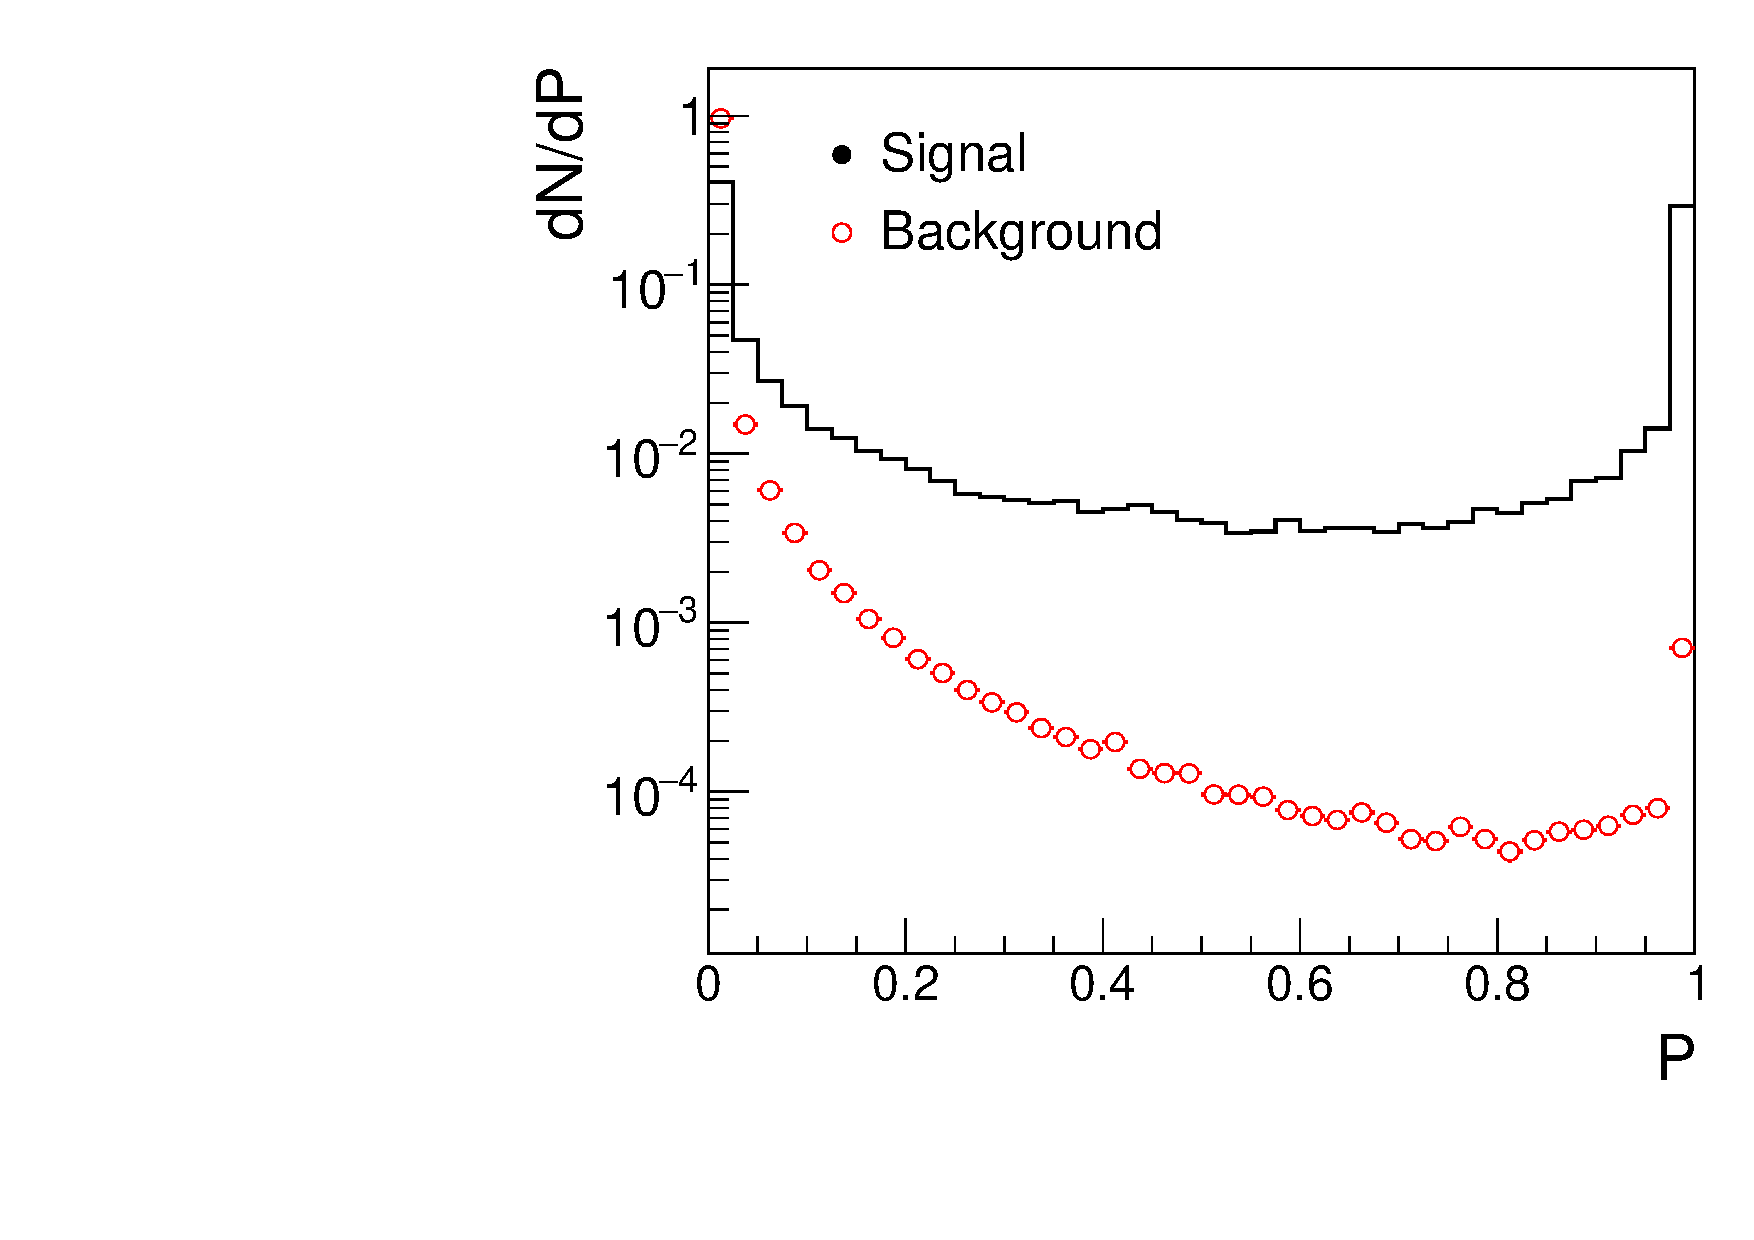
\includegraphics[width=0.48\textwidth]{plots/signal_vs_background_memLR_unsmeared.pdf}
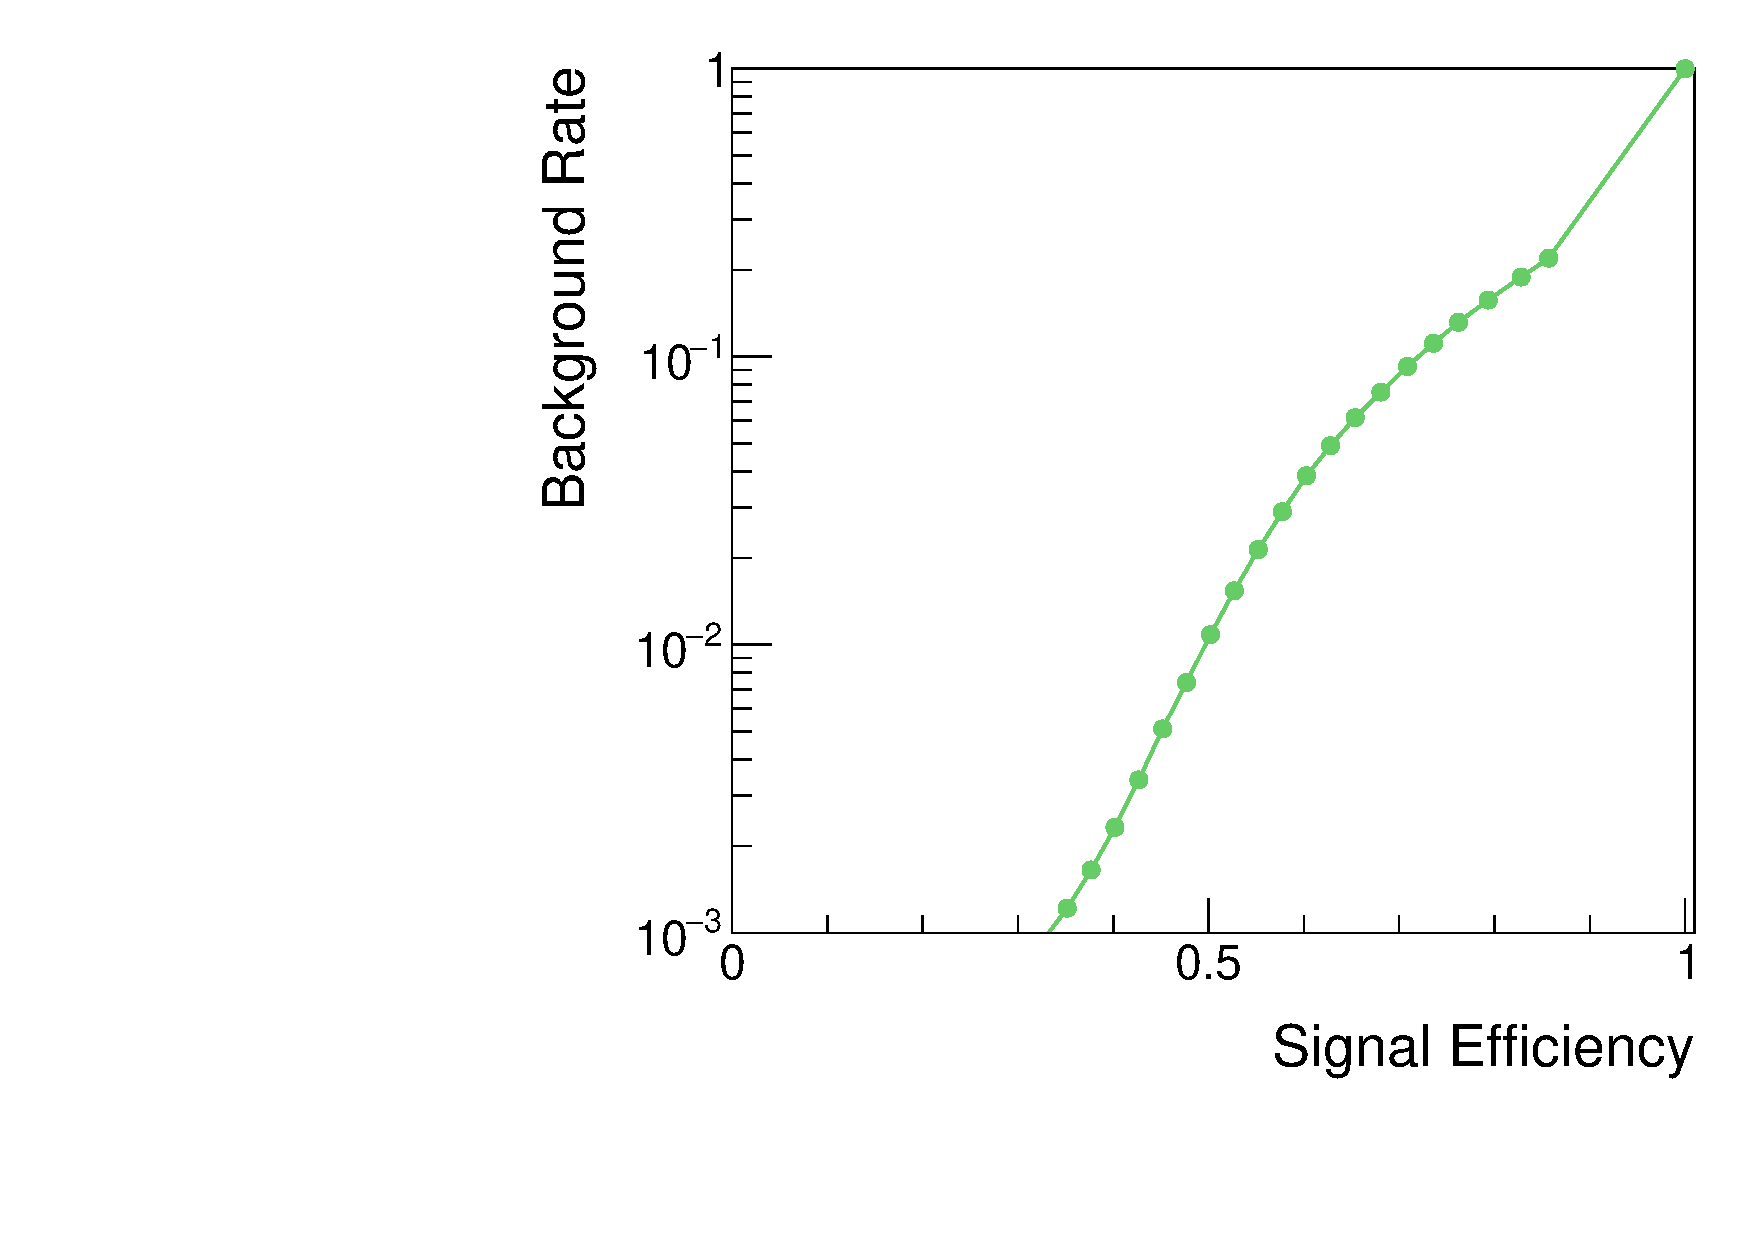
\includegraphics[width=0.48\textwidth]{plots/ROC_unsmeared.pdf}
\fi
\caption{
  Left: Distribution in the LR $P(\vecy)$ given by Eq.~(\ref{eq:memLR}), obtained for $\dihiggs$ signal and for $\ttbar$ background events.
  Right: Graph of background rate versus signal efficiency (``ROC curve''), obtained by applying a cut on the distribution shown on the left
  and varying the cut threshold.
  The signal and background events are studied on MC-truth level.
}
\label{fig:memLR_and_ROC_unsmeared}
\end{figure}

We will allude to this signal efficiency and background rejection in the following,
when quantifying the effect of the experimental resolution on the energy of $\Pbottom$-jets and on the hadronic recoil,
as well as of the misidentification of light-quark and gluon jets as $\Pbottom$-jets.


\subsection{Effect of experimental resolution on \texorpdfstring{$\Pbottom$}{b}-jets and hadronic recoil}

The effect of the experimental resolution on the distributions in the LR $P(\vecy)$ and on the ROC curve is estimated
by randomly sampling the energy $E$ of $\Pbottom$-jets and the components $\pX^{\rho}$ and $\pY^{\rho}$ of the hadronic recoil from the corresponding TF,
given by Eqs.~(\ref{eq:TF_b}) and~(\ref{eq:TF_hadRecoil}), and recomputing the LR $P(\vecy)$ for each such variation.
The resolutions on the energy of $\Pbottom$-jets and on the transverse momentum components of the hadronic recoil 
are given by Eqs.~(\ref{eq:resolution_b}) and~(\ref{eq:resolution_rho}).
The resulting distributions in $P(\vecy)$ are shown for $\dihiggs$ signal and $\ttbar$ background events in Fig.~\ref{fig:memLR_smeared}.
The distributions are compared to those obtained for the case that the LR $P(\vecy)$ is computed on MC-truth level.
The effect on the ROC curve is depicted in Fig.~\ref{fig:ROC_smeared}.
As one can see in the figure, the experimental resolutions have only a small effect on the separation between the $\dihiggs$ signal and the $\ttbar$ background,
relative to the performance achieved on MC-truth level.

\begin{figure}
\ifx\ver\verPreprint
\setlength{\unitlength}{1mm}
\begin{center}
\begin{picture}(160,78)(0,0)
\put(0.0, 0.0){\mbox{\includegraphics*[height=78mm]
 {plots/effectOfSmearing_memLR_signal.pdf}}}
\put(81.0, 0.0){\mbox{\includegraphics*[height=78mm]
 {plots/effectOfSmearing_memLR_background.pdf}}}
\end{picture}
\end{center}
\fi
\ifx\ver\verPAPER
\centering
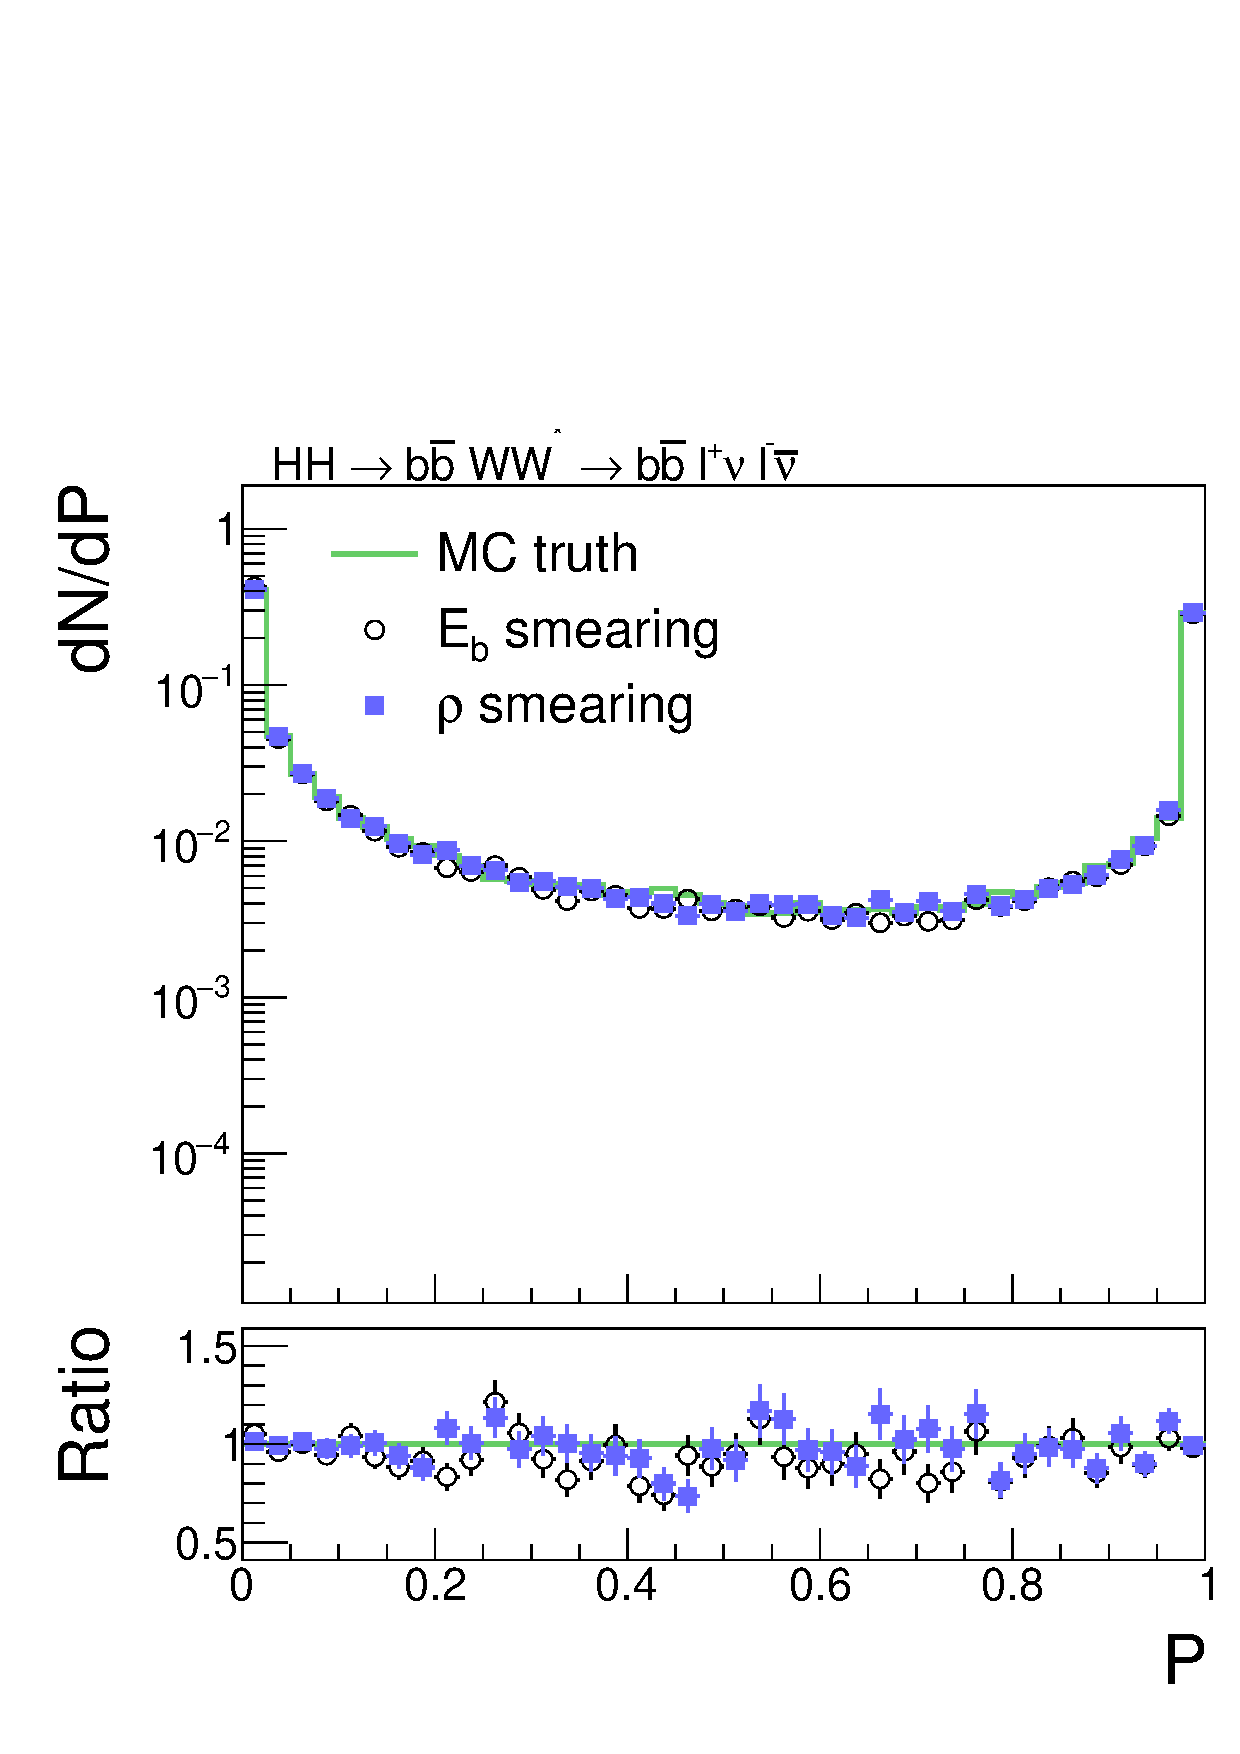
\includegraphics[width=0.48\textwidth]{plots/effectOfSmearing_memLR_signal.pdf}
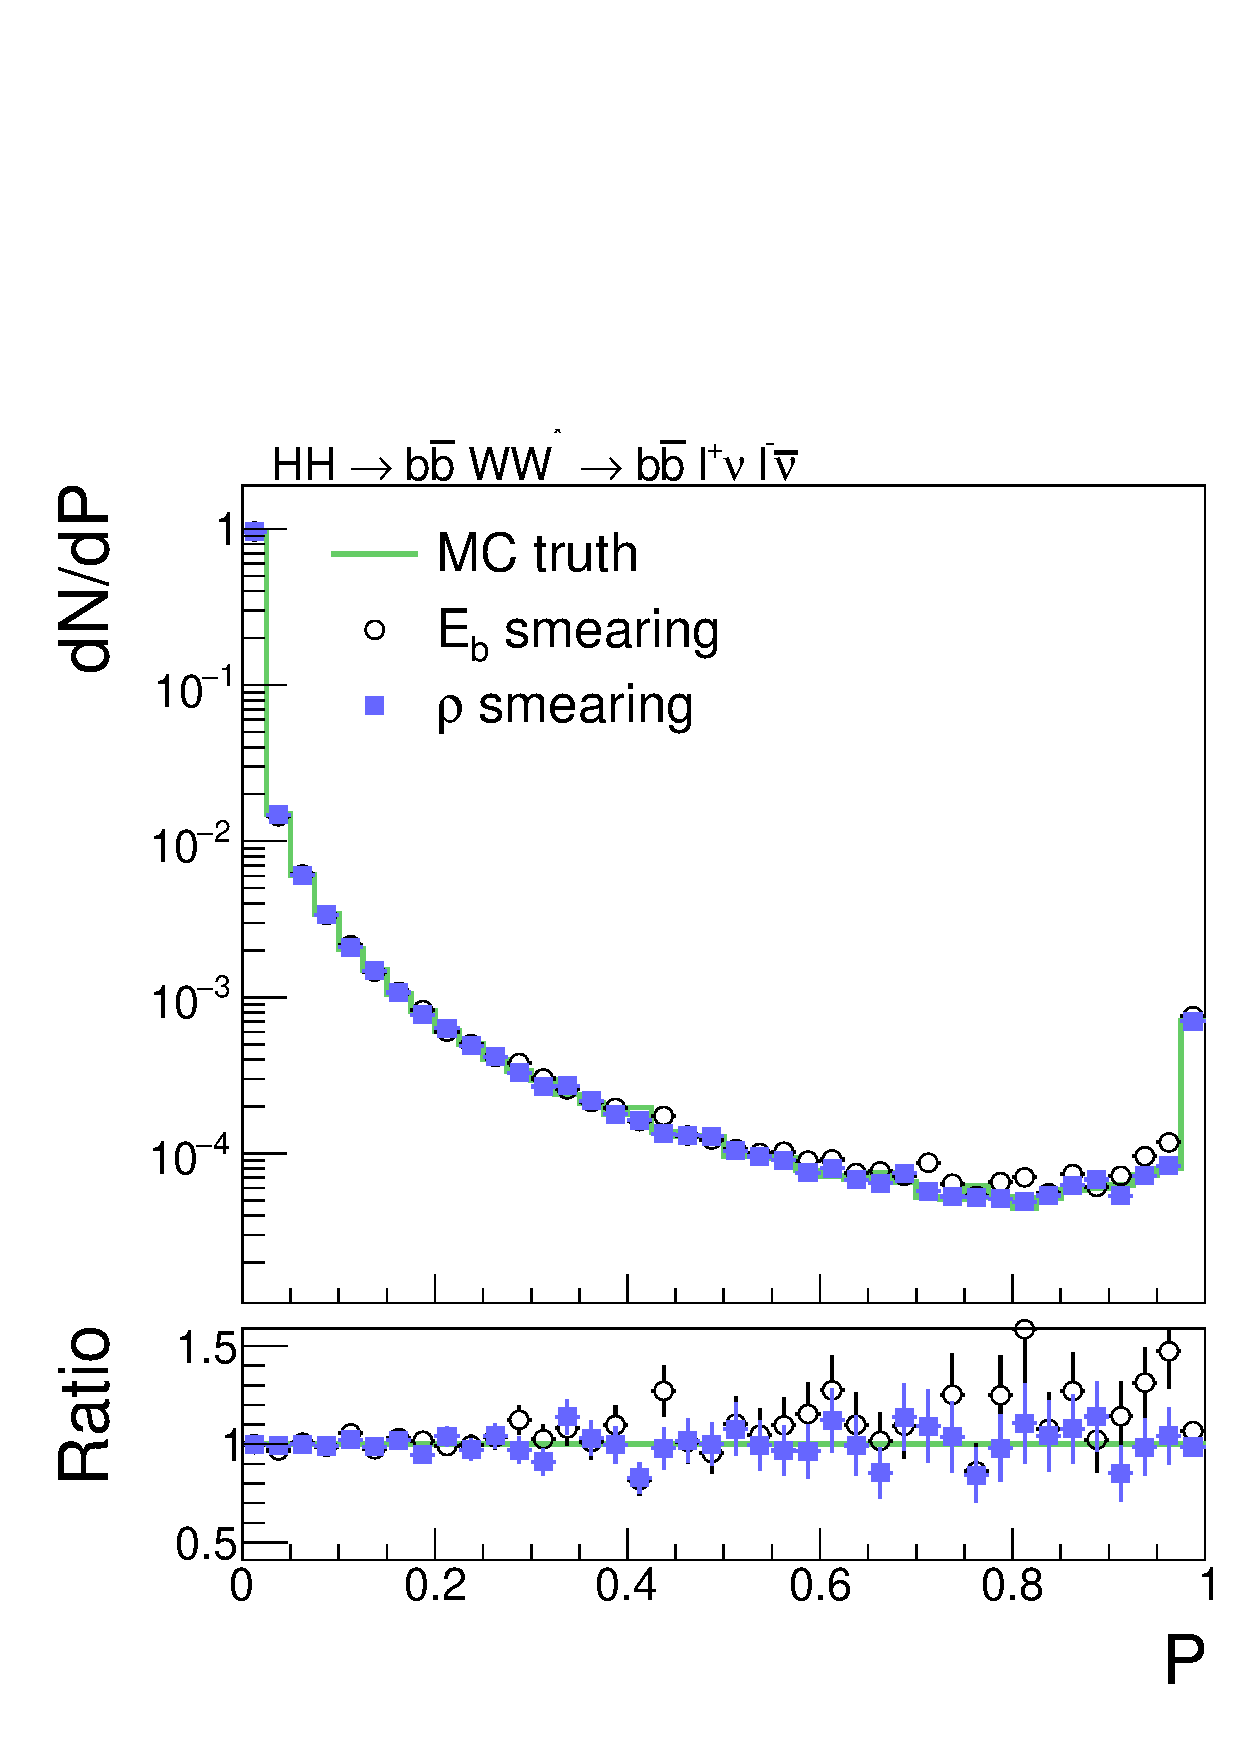
\includegraphics[width=0.48\textwidth]{plots/effectOfSmearing_memLR_background.pdf}
\fi
\caption{
  Effect of the experimental resolutions on the energy of $\Pbottom$-jets (``$E_{\Pbottom}$ smearing'') and on the hadronic recoil (``$\rho$ smearing'') 
  on the distribution in the LR $P(\vecy)$ obtained for simulated $\dihiggs$ signal (left) and $\ttbar$ background (right) events.
}
\label{fig:memLR_smeared}
\end{figure}

\begin{figure}
\ifx\ver\verPreprint
\setlength{\unitlength}{1mm}
\begin{center}
\begin{picture}(160,78)(0,0)
\put(39.5, 0.0){\mbox{\includegraphics*[height=78mm]
 {plots/effectOfSmearing_ROC.pdf}}}
\end{picture}
\end{center}
\fi
\ifx\ver\verPAPER
\centering
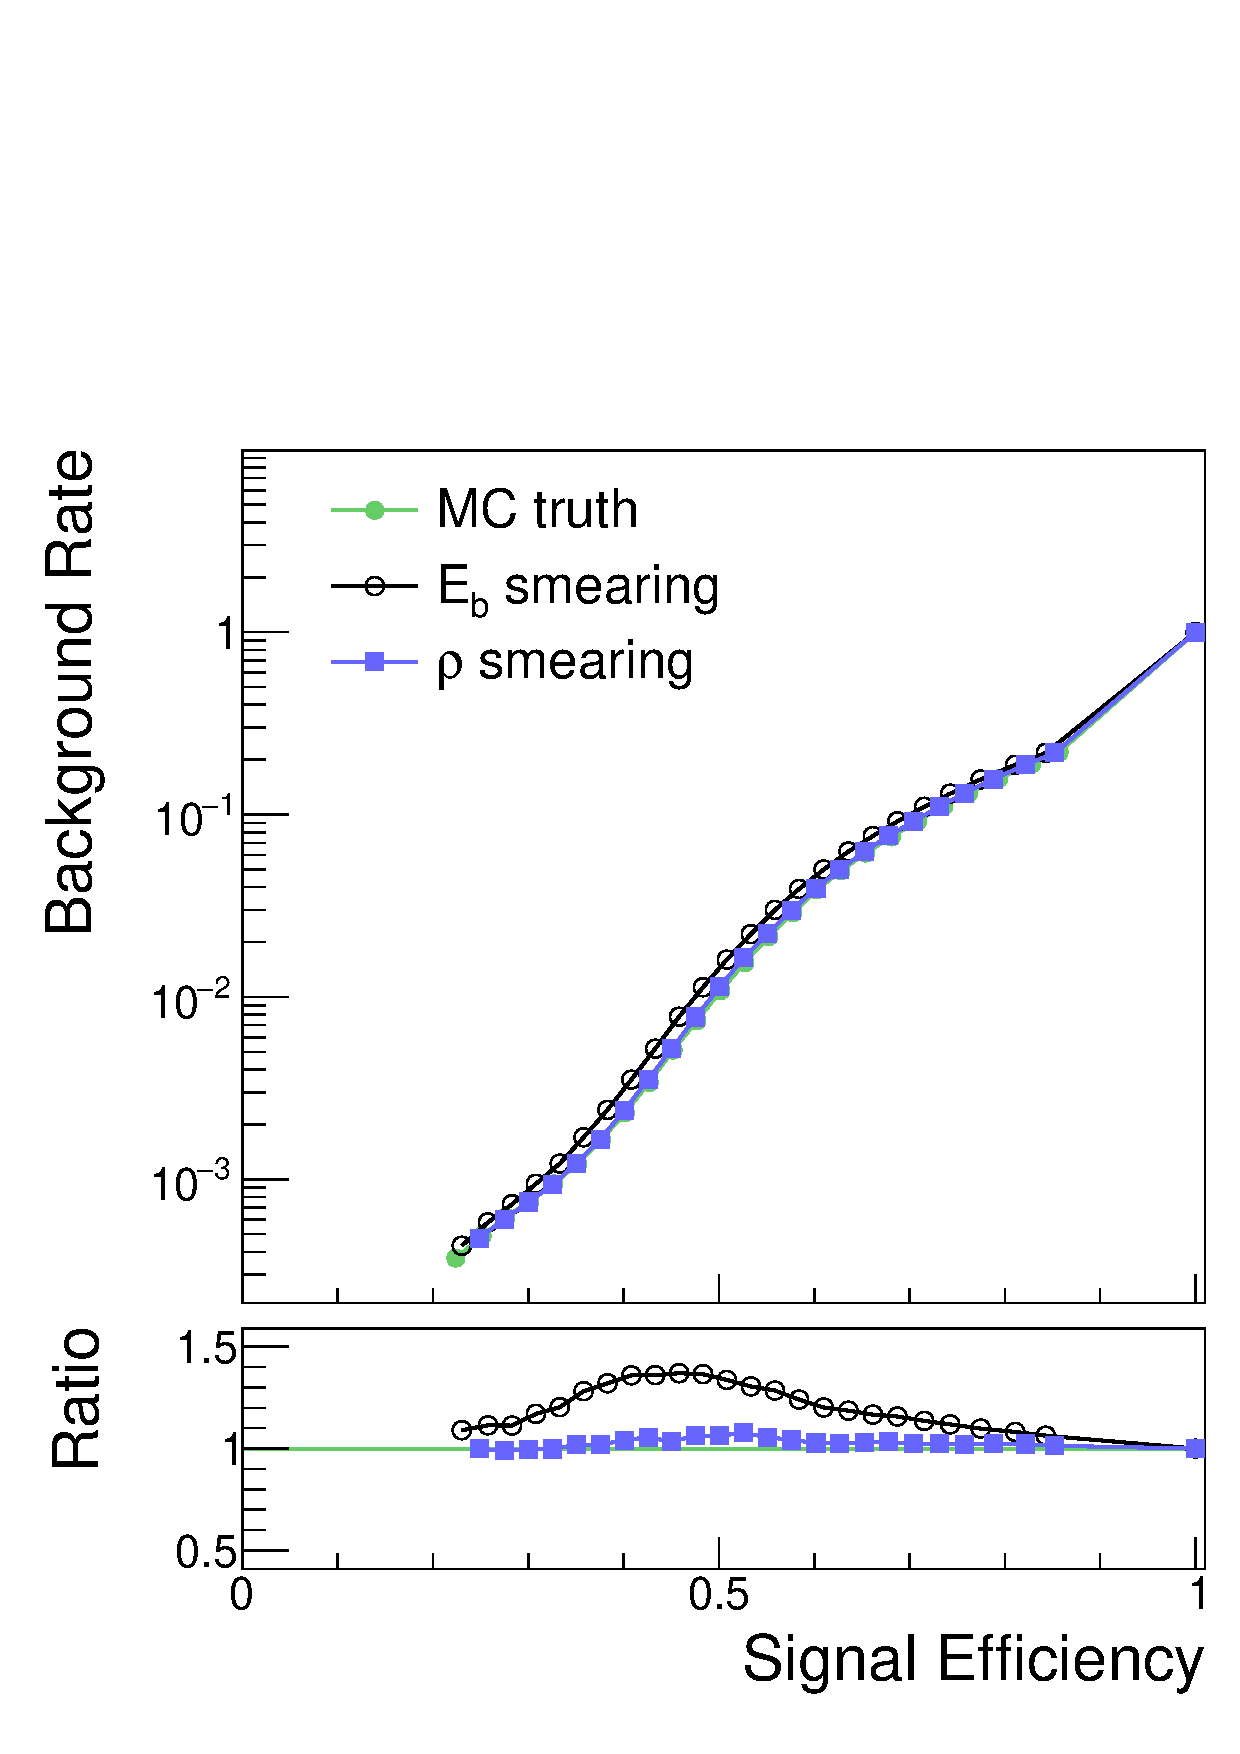
\includegraphics[width=0.48\textwidth]{plots/effectOfSmearing_ROC.pdf}
\fi
\caption{
  Effect of the experimental resolutions on the energy of $\Pbottom$-jets (``$E_{\Pbottom}$ smearing'') and on the hadronic recoil (``$\rho$ smearing'') 
  on the ROC curve. 
}
\label{fig:ROC_smeared}
\end{figure}


\subsection{Effect of misidentifying light-quark and gluon jets as \texorpdfstring{$\Pbottom$}{b}-jets}

Besides the experimental resolution on the $\Pbottom$-jet energy and on the hadronic recoil,
reconstruction effects may degrade the separation between the $\dihiggs$ signal and the $\ttbar$ background
in case one of the two $\Pbottom$-jets that are produced in the decays of the $\PHiggs$ boson or of the top quark pair
fails to get reconstructed,
and a light-quark or gluon jet gets misidentified as $\Pbottom$-jet.
The light-quark or gluon jet can be produced by either ISR or FSR, from the underlying event, 
or from additional proton-proton interactions (pileup) occurring in the same bunch-crossing as the hard-scattering interaction.
The efficiency to identify $\Pbottom$-jets typically amounts to $60$-$70\%$ at the ATLAS and CMS experiments,
for a misidentification rate for light-quark and gluon jets of order $1\%$~\cite{Aad:2015ydr,BTV-16-002}.

We simulate the effect that one of the two true $\Pbottom$-jets fails to get reconstructed and a light-quark or gluon jet gets misidentified as $\Pbottom$-jet
by replacing $10\%$ of true $\Pbottom$-jets by randomly selected light-quark or gluon jets produced by either ISR or FSR, or from the underlying event 
(our simulated samples of signal and background events do not include pileup). 
We then compare the distributions in the LR $P(\vecy)$ thus obtained with the corresponding distributions obtained for the case that both $\Pbottom$-jets are genuine $\Pbottom$-jets.
The results are shown in Fig.~\ref{fig:memLR_fakeBJet}.
We observe that the misidentification of light-quark and gluon jets as $\Pbottom$-jets has a sizeable effect on the LR $P(\vecy)$.
More specifically, the distribution in $P(\vecy)$ obtained for signal events becomes significantly more background-like
in case a light-quark or gluon jet is misidentified as $\Pbottom$-jet.
Similarly, the distribution in $P(\vecy)$ obtained for background events becomes significantly more signal-like.
As a result, the separation between the $\dihiggs$ signal and the $\ttbar$ background degrades significantly,
resulting in a sizeable loss in performance of the MEM, whenever a light-quark or gluon jet is misidentified as $\Pbottom$-jet.
The loss in performance can be seen clearly in the ROC curve, which is shown in Fig.~\ref{fig:ROC_fakeBJet}.

\begin{figure}
\ifx\ver\verPreprint
\setlength{\unitlength}{1mm}
\begin{center}
\begin{picture}(160,66)(0,0)
\put(-1.0, 0.0){\mbox{\includegraphics*[height=66mm]
 {plots/effectOfFakes_2histograms_memLR_signal.pdf}}}
\put(80.0, 0.0){\mbox{\includegraphics*[height=66mm]
 {plots/effectOfFakes_2histograms_memLR_background.pdf}}}
\end{picture}
\end{center}
\fi
\ifx\ver\verPAPER
\centering
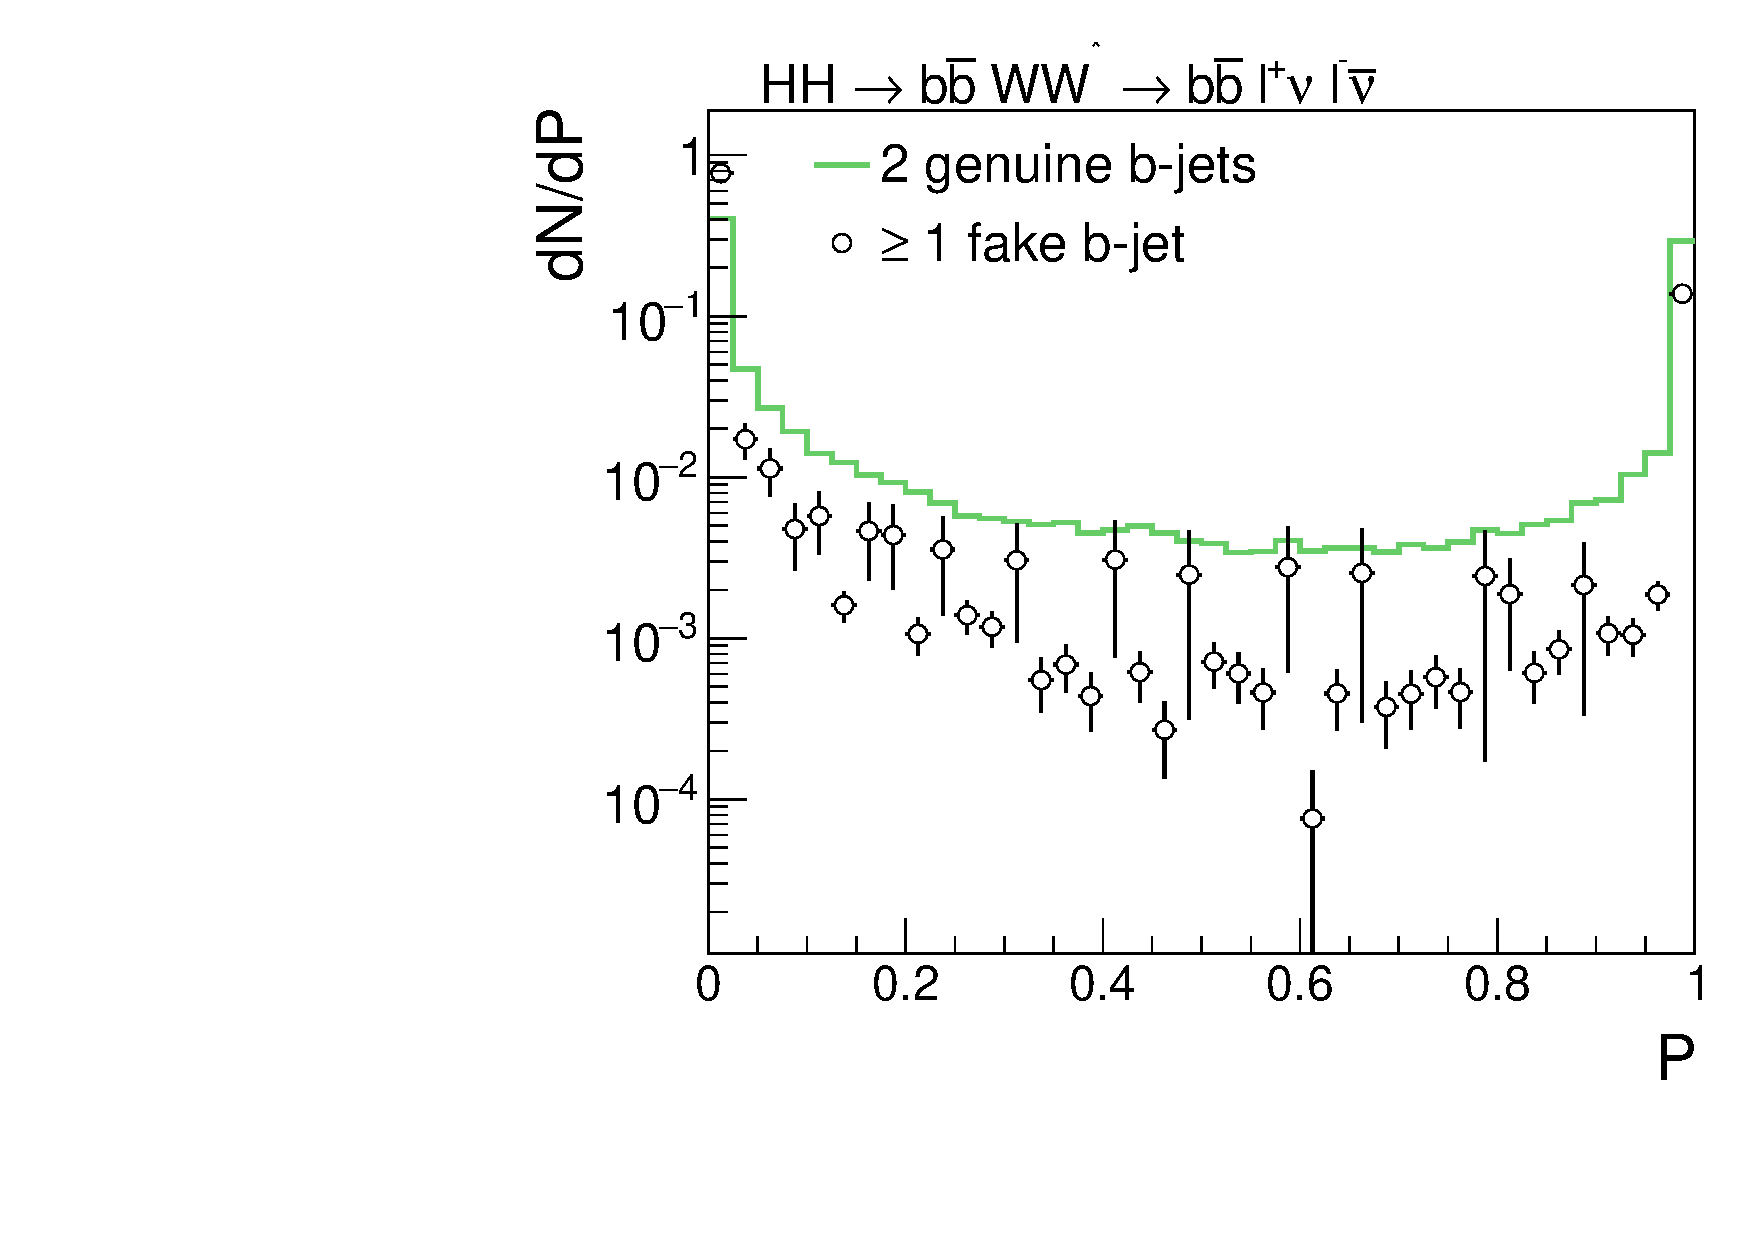
\includegraphics[width=0.48\textwidth]{plots/effectOfFakes_2histograms_memLR_signal.pdf}
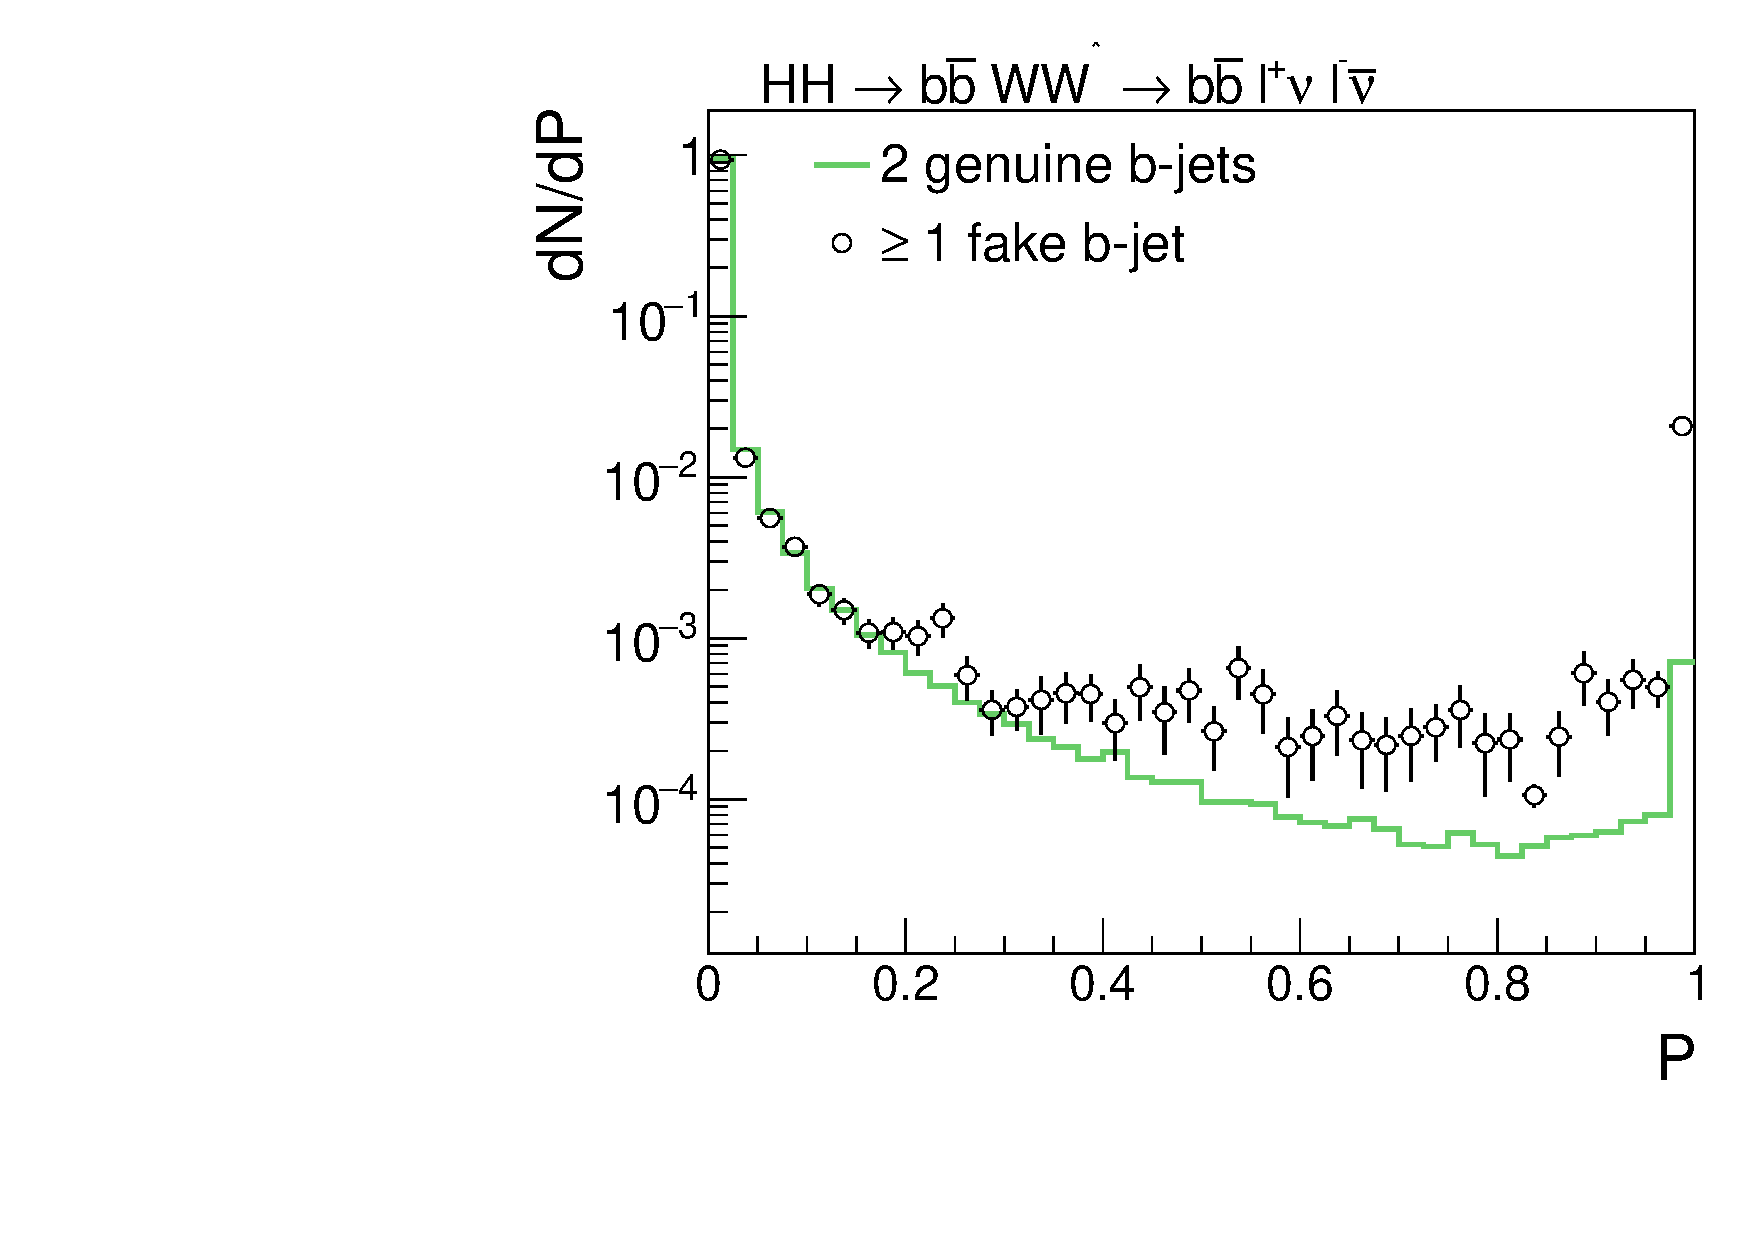
\includegraphics[width=0.48\textwidth]{plots/effectOfFakes_2histograms_memLR_background.pdf}
\fi
\caption{
  Effect of misidentifying a light-quark or gluon jet (``fake'') as $\Pbottom$-jet
  on the distribution in the LR $P(\vecy)$ obtained for simulated $\dihiggs$ signal (left) and $\ttbar$ background (right) events.
}
\label{fig:memLR_fakeBJet}
\end{figure}

\begin{figure}
\ifx\ver\verPreprint
\setlength{\unitlength}{1mm}
\begin{center}
\begin{picture}(160,67)(0,0)
\put(39.5, 0.0){\mbox{\includegraphics*[height=67mm]
 {plots/effectOfFakes_2graphs_ROC.pdf}}}
\end{picture}
\end{center}
\fi
\ifx\ver\verPAPER
\centering
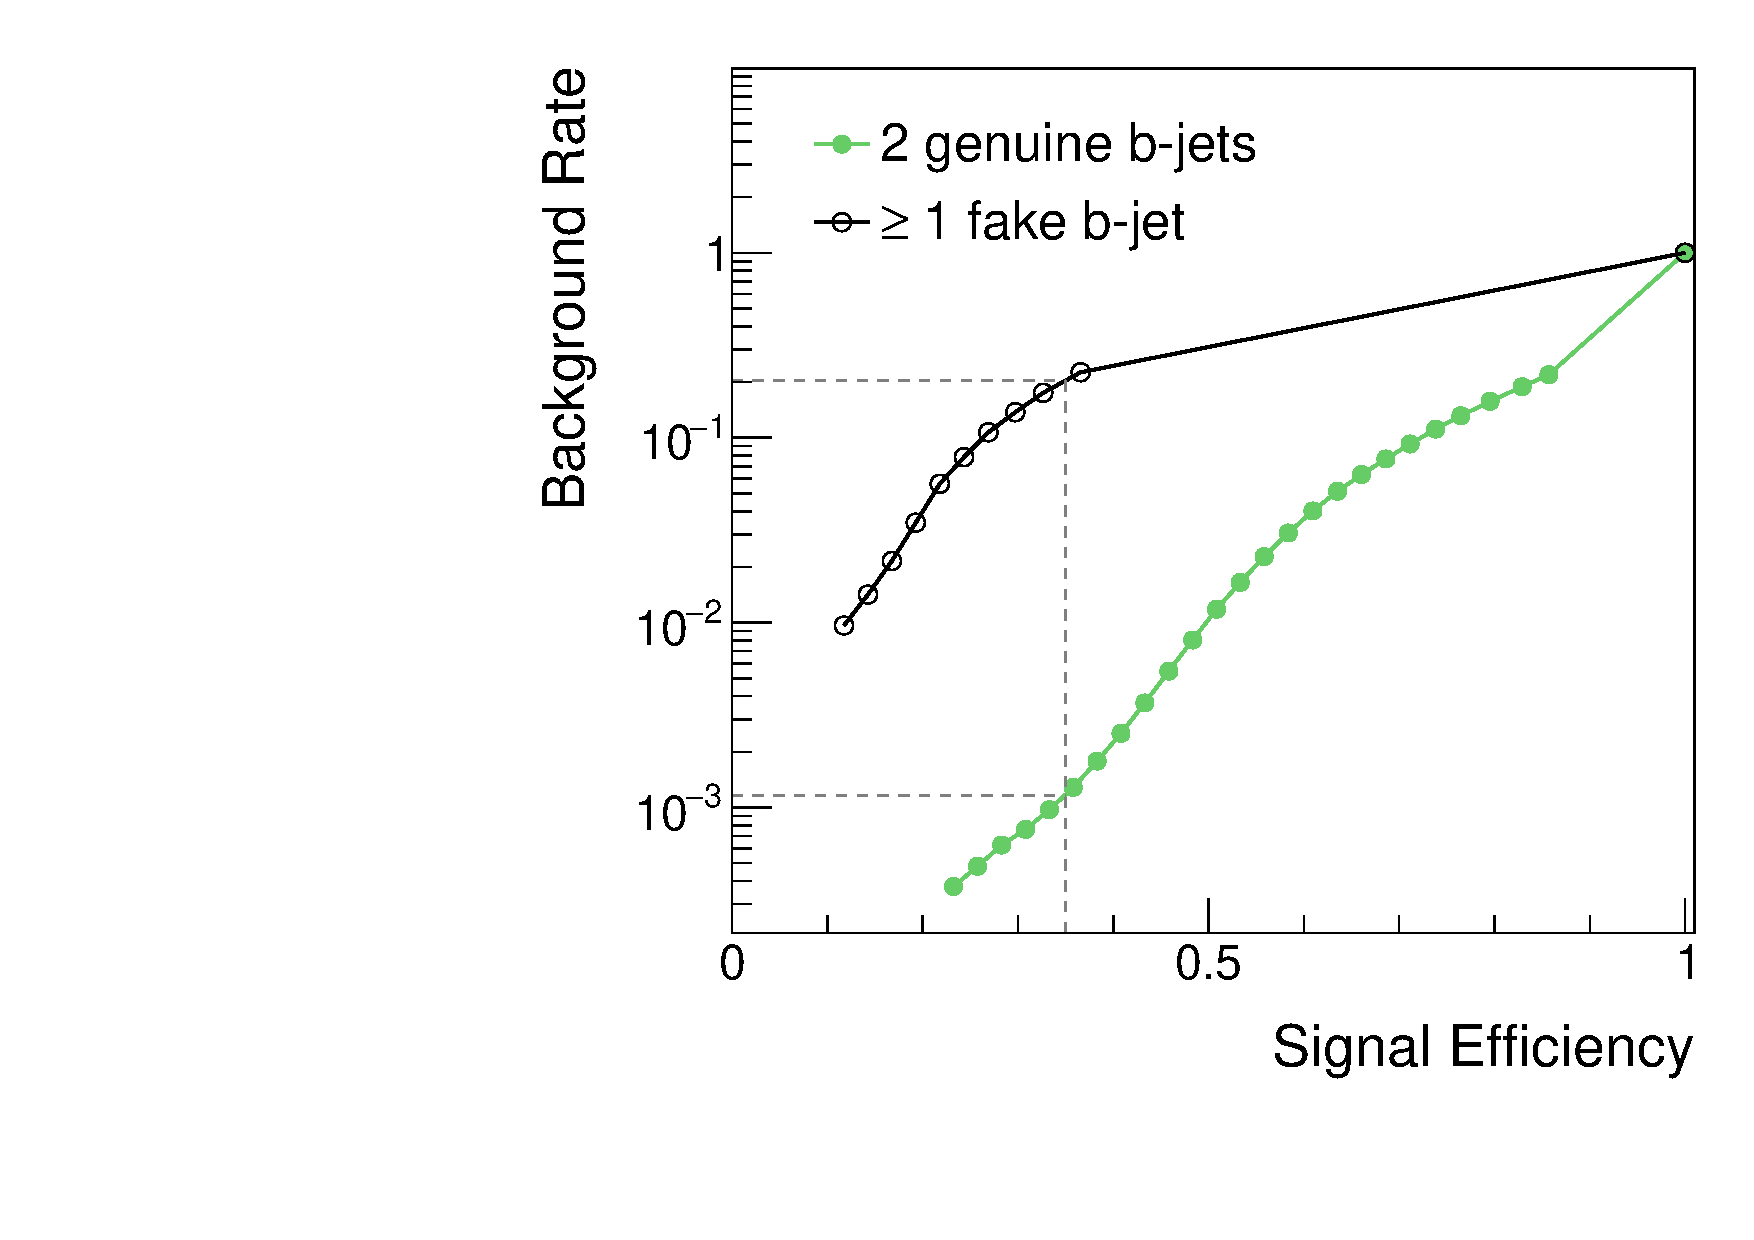
\includegraphics[width=0.48\textwidth]{plots/effectOfFakes_2graphs_ROC.pdf}
\fi
\caption{
  Effect of misidentifying a light-quark or gluon jet (``fake'') as $\Pbottom$-jet
  on the ROC curve.
}
\label{fig:ROC_fakeBJet}
\end{figure}

Compared to the effect of the experimental resolution on the $\Pbottom$-jet energy and on the momentum of the hadronic recoil,
the loss in signal-to-background separation arising from the misidentification of a light-quark or gluon jet as a $\Pbottom$-jet
is much more severe. 

The magnitude of the effect warrants further investigations concerning its origin and the development of approaches to mitigate the effect.
In Fig.~\ref{fig:probS_and_probB_fakeBJet} we show the distributions in the PDs $w_{0}(\vecy)$ and $w_{1}(\vecy)$
that quantify the level of compatibility with the signal and background hypotheses.
The distributions in $w_{0}(\vecy)$ and in $w_{1}(\vecy)$ are shown separately 
for signal and background events in which at least one of the two $\Pbottom$-jets is due to the misidentification of a light-quark or gluon jet
and for events in which both $\Pbottom$-jets are genuine $\Pbottom$-jets.
We observe that the distributions in the probability density for the ``correct'' hypothesis 
($w_{0}(\vecy)$ for signal and $w_{1}(\vecy)$ for background events)
are more susceptible to the misidentification of light-quark and gluon jets as $\Pbottom$-jets than the distributions in the PD for the ``wrong'' hypothesis 
($w_{1}(\vecy)$ for signal and $w_{0}(\vecy)$ for background events).
The distribution in the PD $w_{0}(\vecy)$ for signal events to be classified as signal is affected the most.
The large magnitude of the effect on $w_{0}(\vecy)$ is explained by the presence of a BW propagator in the ME $\mathcal{M}_{0}(\vecphat)$ for the signal hypothesis,
which enforces that the mass of the pair of $\Pbottom$-jets equals $m_{\PHiggs}$.
The $\delta$-function introduced into the integrand of Eq.~(\ref{eq:mem3}) via the transformations described in Section~\ref{sec:appendix_bEn_Hbb} of the appendix
guarantees the compliance with the $\PHiggs$ boson mass constraint,
but introduces large ``pulls'' in the TF $W(E|\Ehat)$ for the $\Pbottom$-jet energy,
in case a light-quark or gluon jet gets misidentified as $\Pbottom$-jet,
which diminish the value of the integrand.

\begin{figure}
\ifx\ver\verPreprint
\setlength{\unitlength}{1mm}
\begin{center}
\begin{picture}(160,144)(0,0)
\put(-1.0, 78.0){\mbox{\includegraphics*[height=66mm]
 {plots/effectOfFakes_2histograms_probS_signal.pdf}}}
\put(80.0, 78.0){\mbox{\includegraphics*[height=66mm]
 {plots/effectOfFakes_2histograms_probB_signal.pdf}}}
\put(-1.0, 0.0){\mbox{\includegraphics*[height=66mm]
 {plots/effectOfFakes_2histograms_probS_background.pdf}}}
\put(80.0, 0.0){\mbox{\includegraphics*[height=66mm]
 {plots/effectOfFakes_2histograms_probB_background.pdf}}}
\end{picture}
\end{center}
\fi
\ifx\ver\verPAPER
\centering
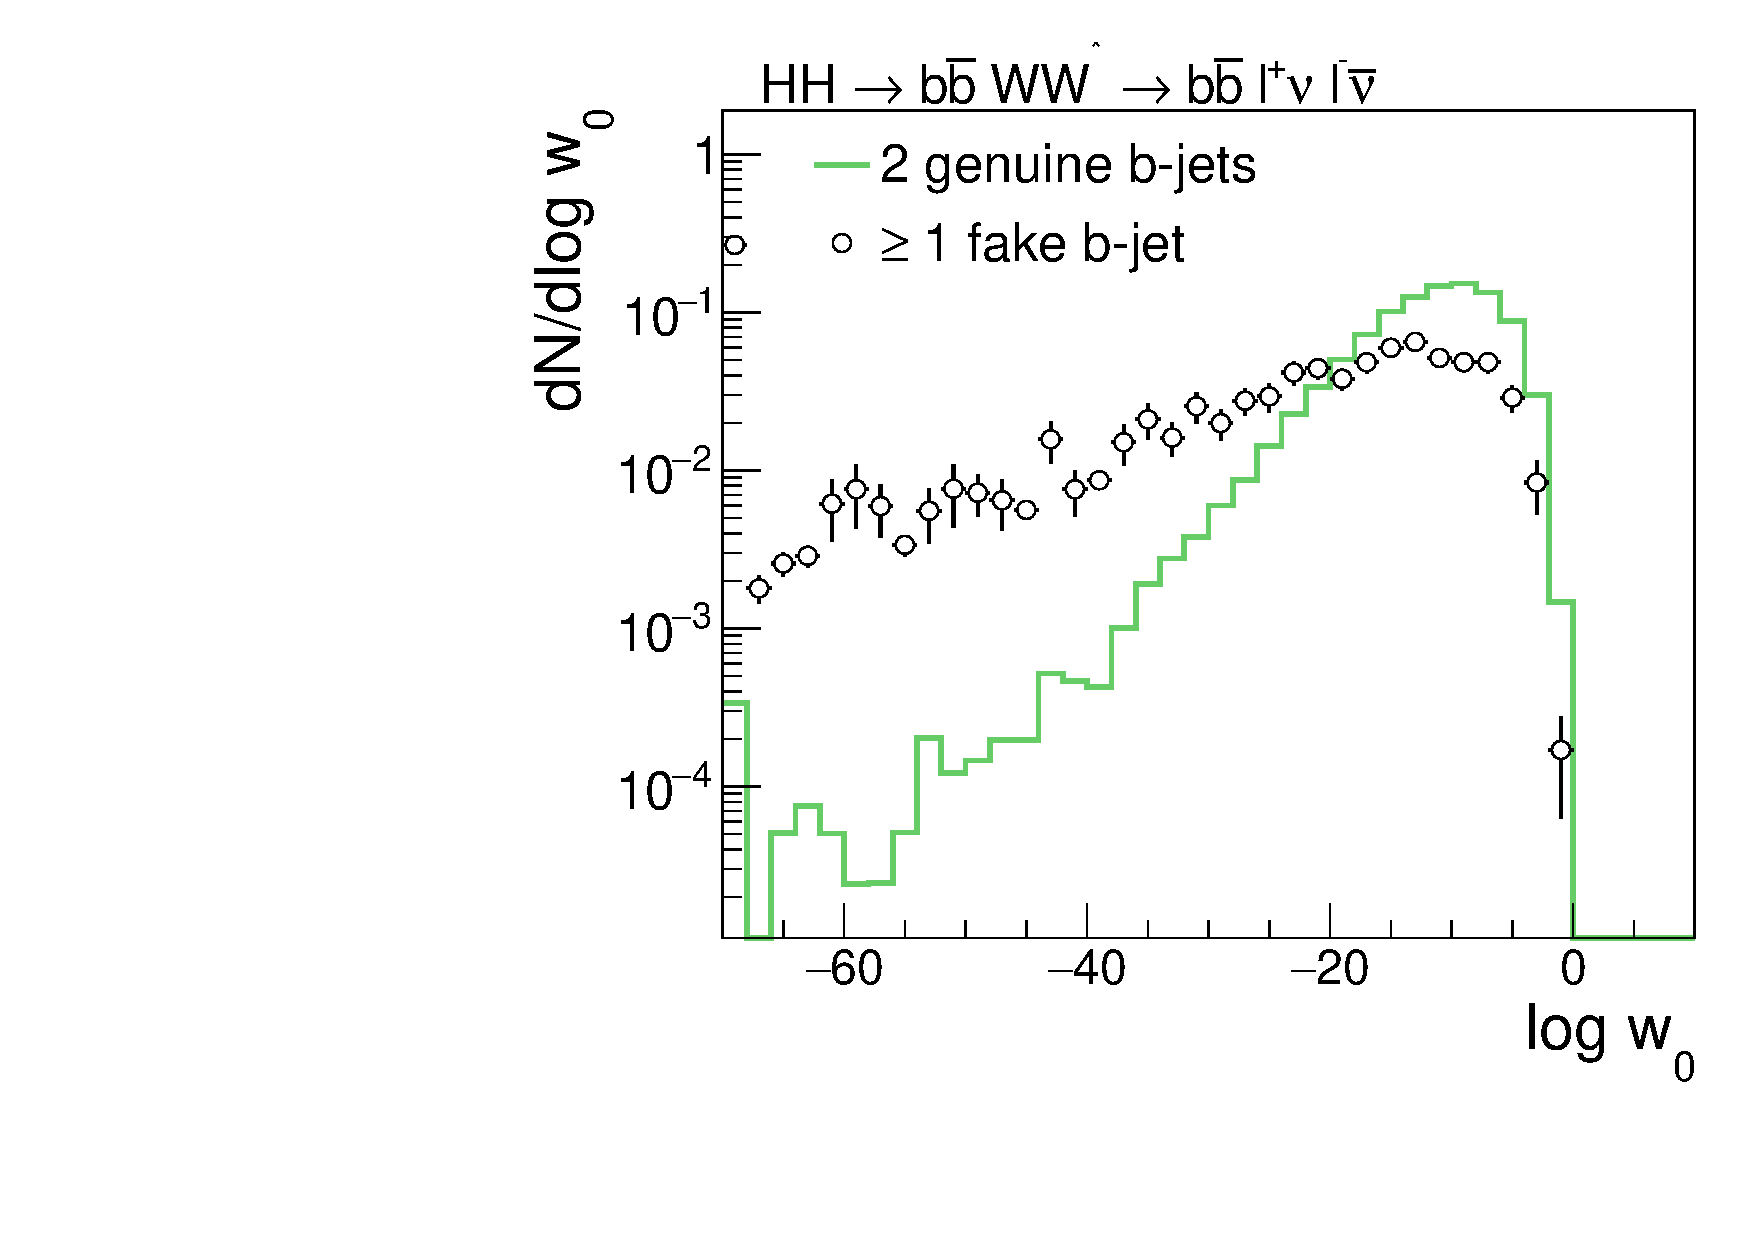
\includegraphics[width=0.48\textwidth]{plots/effectOfFakes_2histograms_probS_signal.pdf}
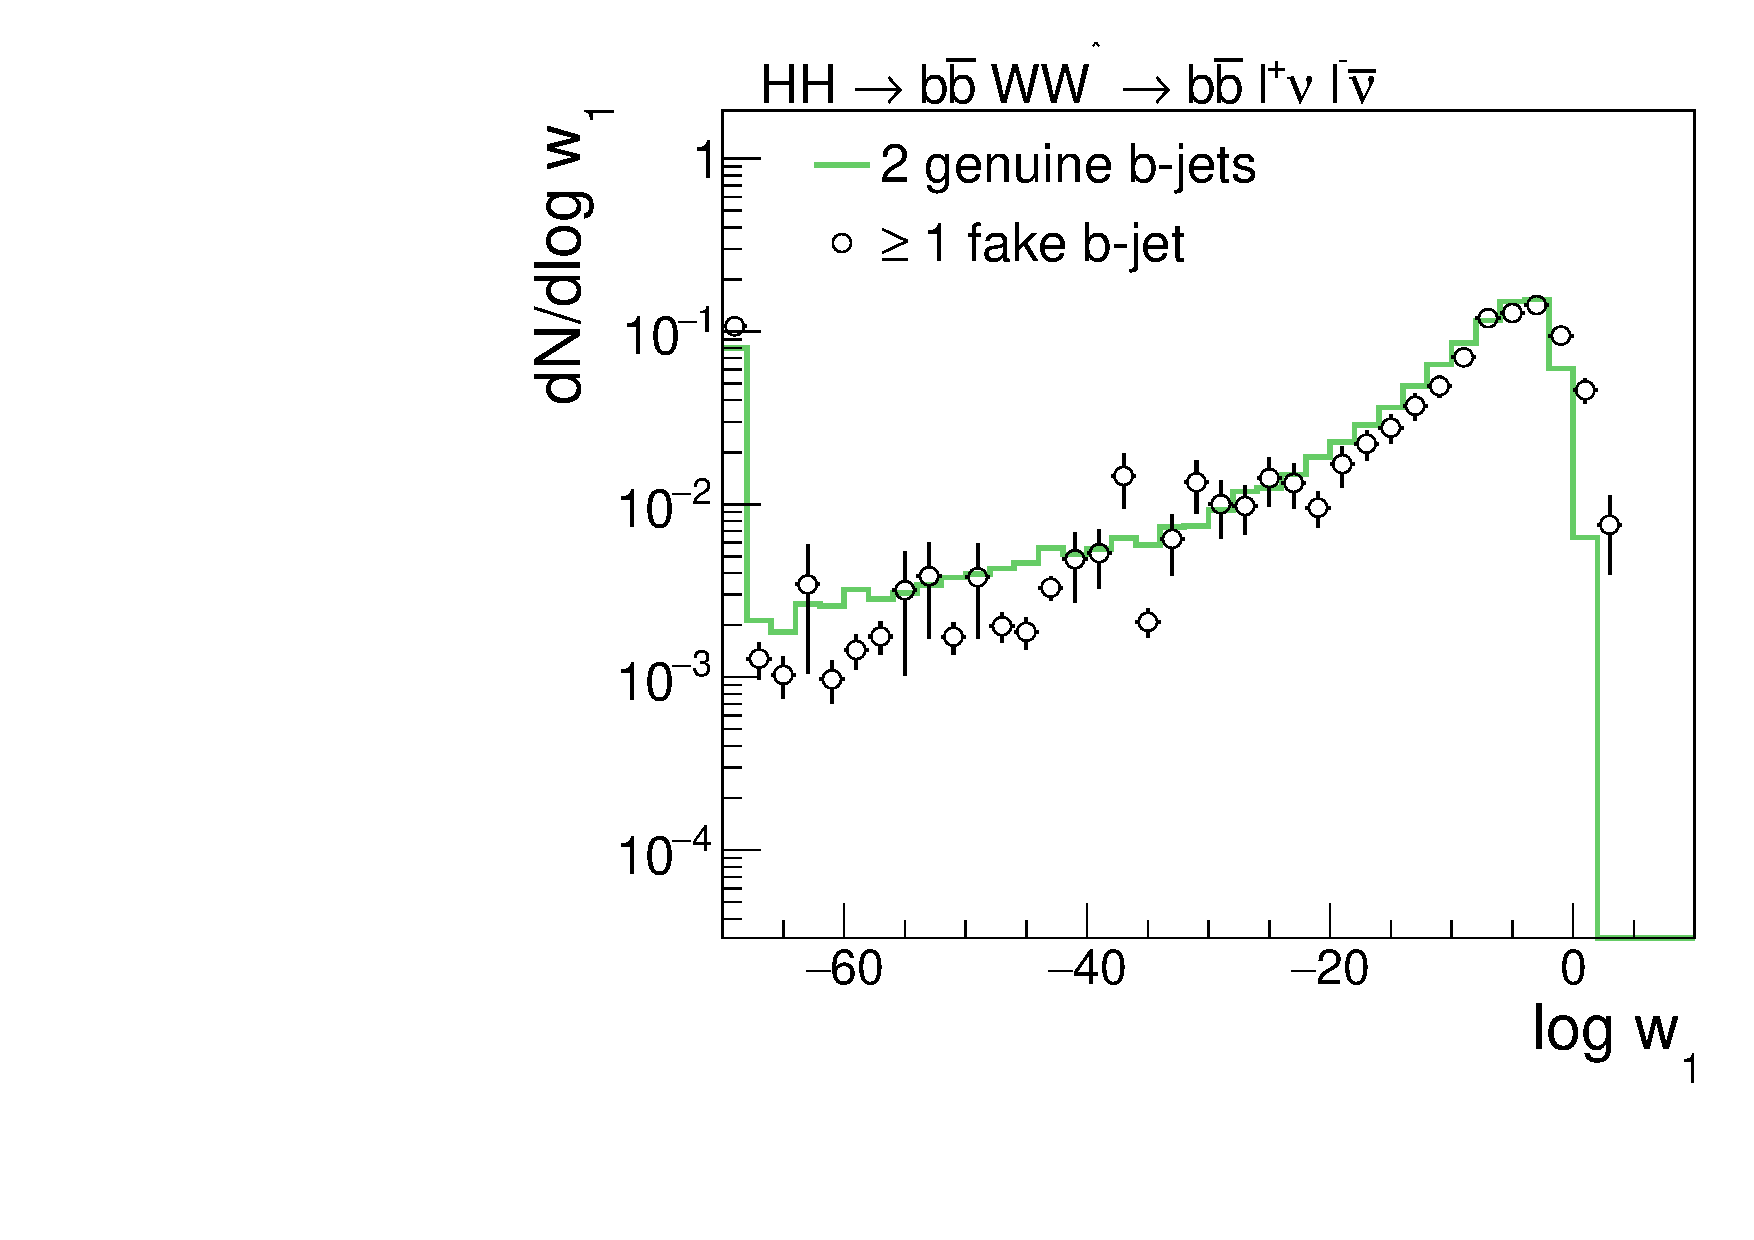
\includegraphics[width=0.48\textwidth]{plots/effectOfFakes_2histograms_probB_signal.pdf}
\hspace{0.04\textwidth}
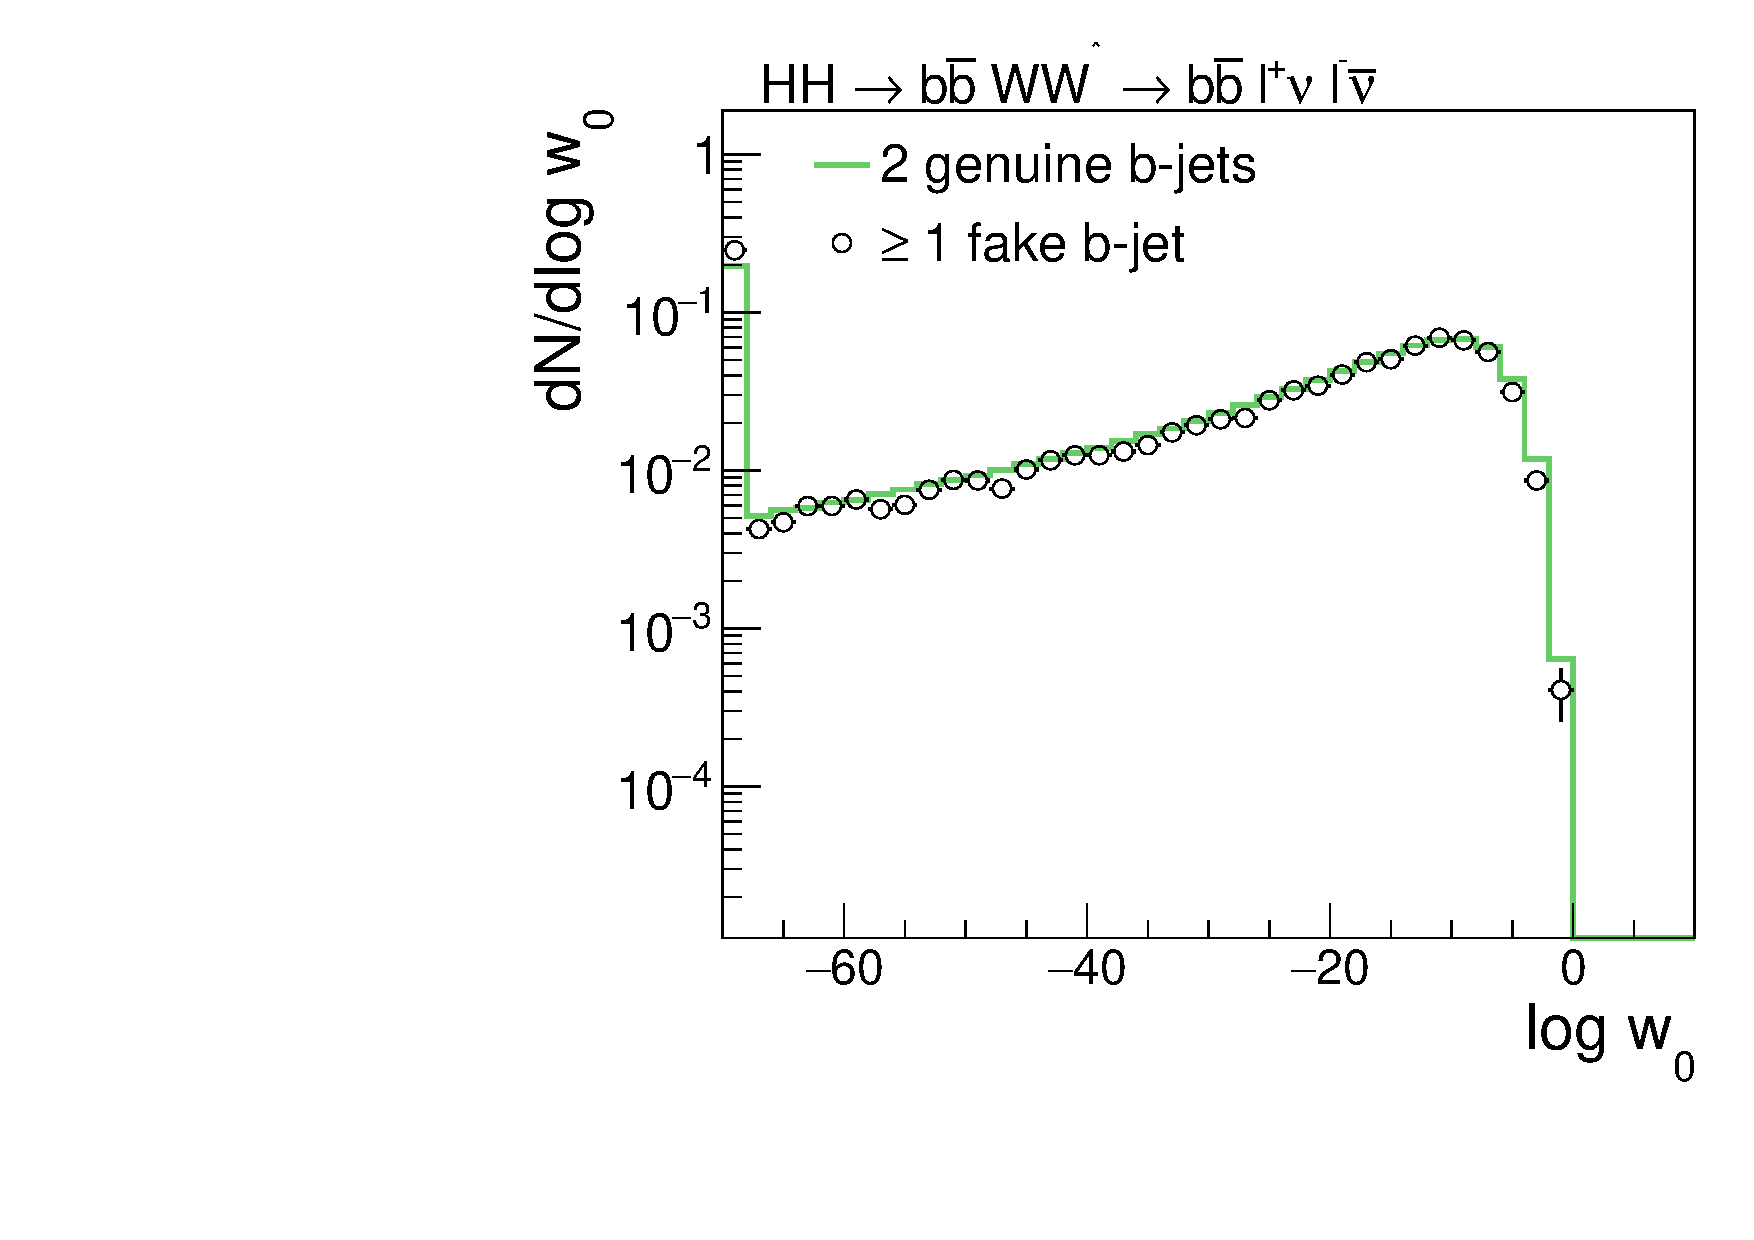
\includegraphics[width=0.48\textwidth]{plots/effectOfFakes_2histograms_probS_background.pdf}
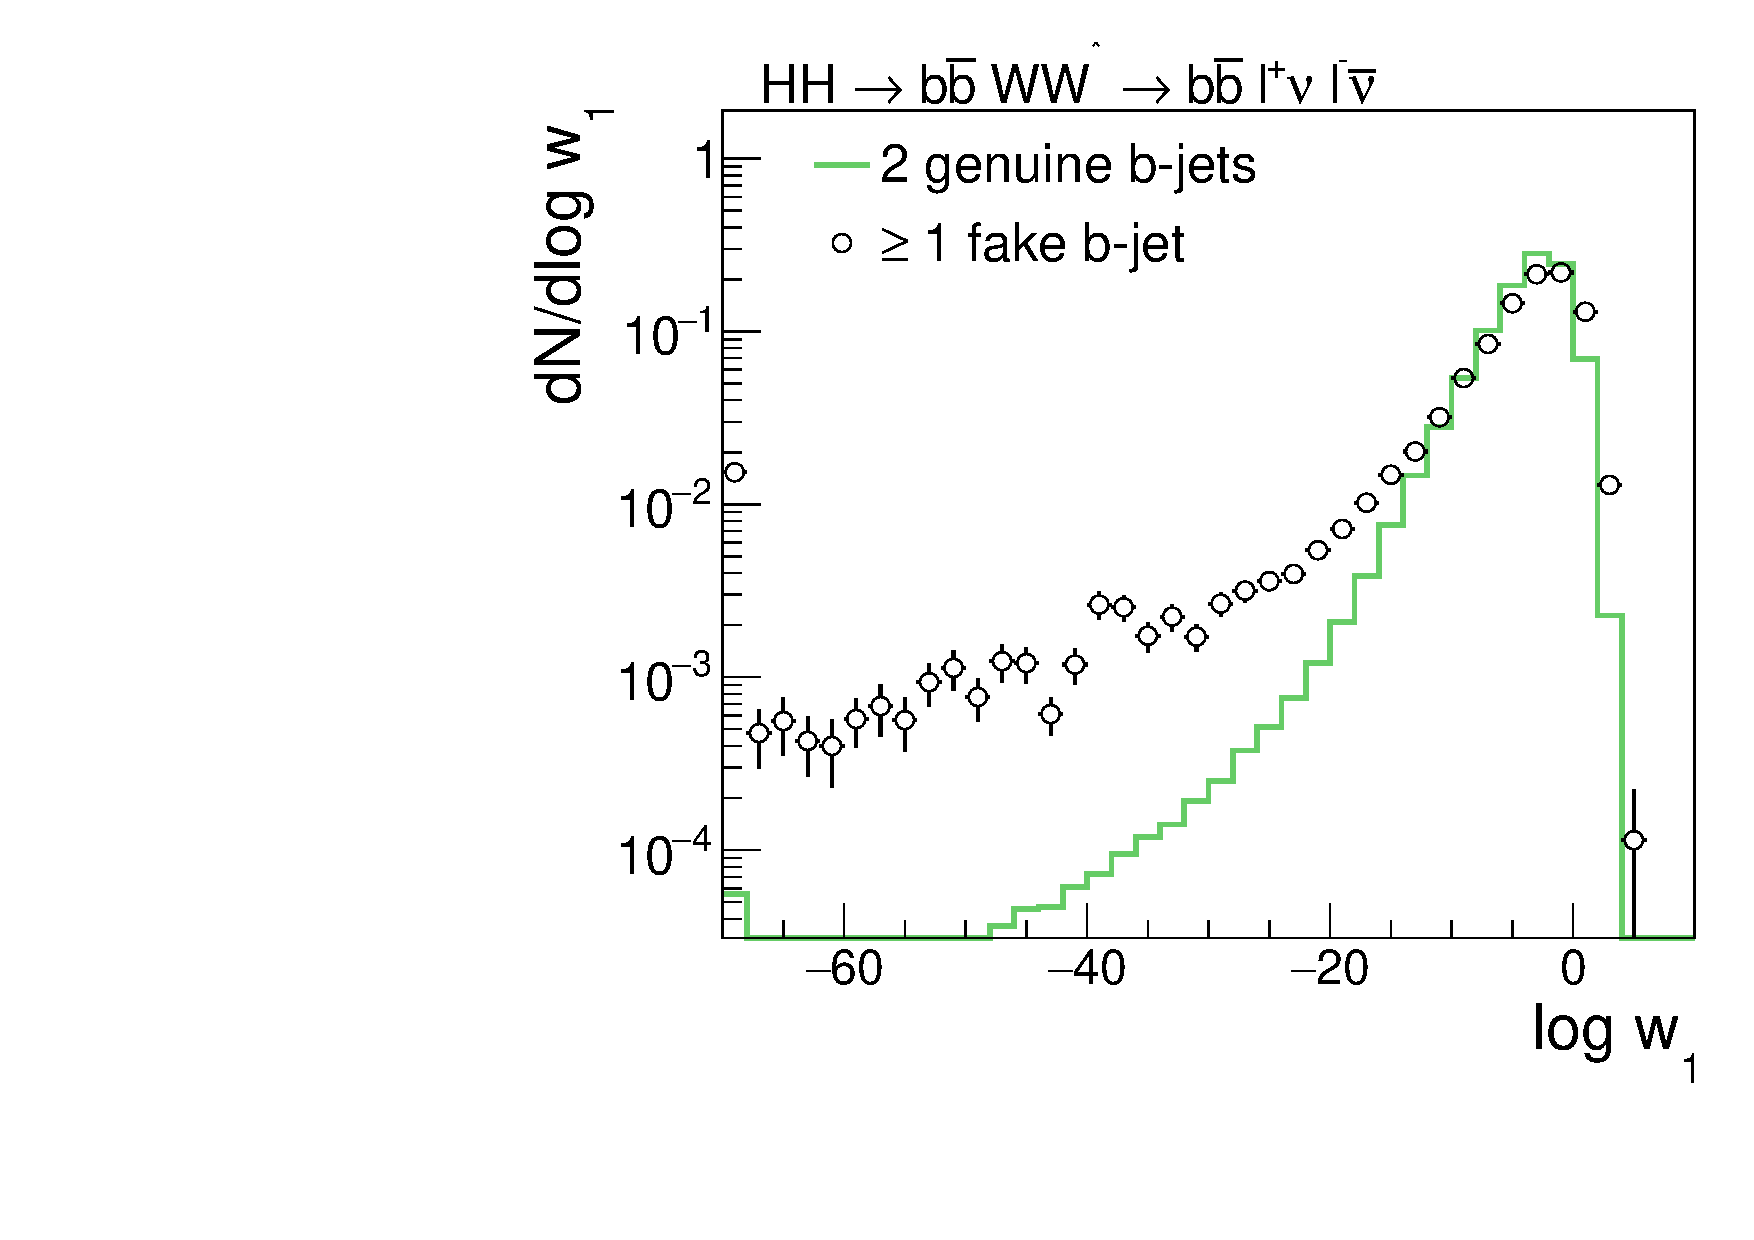
\includegraphics[width=0.48\textwidth]{plots/effectOfFakes_2histograms_probB_background.pdf}
\fi
\caption{
  Effect of misidentifying a light-quark or gluon jet (``fake'') as $\Pbottom$-jet candidate
  on the distribution in the probability densities $w_{0}(\vecy)$ (left) and $w_{1}(\vecy)$ (right)
  obtained for simulated $\dihiggs$ signal (top) and $\ttbar$ background (bottom) events.
}
\label{fig:probS_and_probB_fakeBJet}
\end{figure}

For a signal efficiency of $35\%$, the rate of $\ttbar$ background amounts to about $20\%$
in case a light-quark or gluon jet is misidentified as $\Pbottom$-jet.
This represents an increase in the $\ttbar$ background rate by about two orders of magnitude,
compared to the case that both $\Pbottom$-jets are genuine $\Pbottom$-jets.


\subsection{Mitigation of \texorpdfstring{$\Pbottom$}{b}-jet misidentification effect}

The degradation in the separation of the $\dihiggs$ signal from the $\ttbar$ background can be mitigated 
by marginalizing the expressions for the PDs $w_{0}(\vecy)$ and $w_{1}(\vecy)$ in Eqs.~(\ref{eq:mem_signal}) and~(\ref{eq:mem_background}),
assuming that one of the two true $\Pbottom$-jets failed to get reconstructed.
Marginalization means that the $\Pbottom$-jet variables $E_{\Pbottom}$, $\theta_{\Pbottom}$, and $\phi_{\Pbottom}$
are no longer used in the RHS of these expressions but instead integrated over:
\begin{linenowrapper}
\begin{equation*}
w_{i,\textrm{m}}(\vecy') = \int \, dE_{\Pbottom} \, d\theta_{\Pbottom} \, d\phi_{\Pbottom} \, w_{i}(\vecy) \, ,
\end{equation*}
\end{linenowrapper}
where we have added a subscript $m$ to denote the marginalized PDs and the vector $\vecy'$ equals the vector $\vecy$,
except that the variables $E_{\Pbottom}$, $\theta_{\Pbottom}$, and $\phi_{\Pbottom}$ are absent in the vector $\vecy'$.
Since we do not know whether the jet corresponding to the $\Pbottom$ quark or the one corresponding to the $\APbottom$ quark is the misidentified jet,
we perform the marginalization once with respect to the variables $E_{\Pbottom}$, $\theta_{\Pbottom}$, and $\phi_{\Pbottom}$ 
and once with respect to the variables $E_{\APbottom}$, $\theta_{\APbottom}$, and $\phi_{\APbottom}$ and take the sum.
The computing time required to evaluate the marginalized PDs $w_{0,\textrm{m}}(\vecy')$ and $w_{1,\textrm{m}}(\vecy')$
is similar to the time required to compute the un-marginalized PDs $w_{0}(\vecy')$ and $w_{1}(\vecy')$,
except for the factor two increase that results from the need to perform the marginalization with respect to the $\Pbottom$ and with respect to the $\APbottom$ quark.
The distributions in the marginalized LR $P_{\textrm{m}}(\vecy)$ obtained for the $\dihiggs$ signal as well as for the $\ttbar$ background 
and the corresponding ROC curve is shown in Fig.~\ref{fig:memLR_and_ROC_missingBJet}.
Marginalization reduces the amount of kinematic information, which is utilized for separating the signal from the background,
resulting in an increased overlap in the distributions in $P_{\textrm{m}}(\vecy)$ for the $\dihiggs$ signal and for the $\ttbar$ background,
but also makes the distributions less susceptible to the case that one of the true $\Pbottom$-jets fails to get reconstructed
and a light-quark or gluon jet is misidentified as $\Pbottom$-jet.

\begin{figure}
\ifx\ver\verPreprint
\setlength{\unitlength}{1mm}
\begin{center}
\begin{picture}(160,66)(0,0)
\put(-1.0, 1.0){\mbox{\includegraphics*[height=66mm]
 {plots/effectOfFakes_memLR_missingBJet.pdf}}}
\put(80.0, 0.0){\mbox{\includegraphics*[height=67mm]
 {plots/effectOfFakes_ROC_missingBJet.pdf}}}
\end{picture}
\end{center}
\fi
\ifx\ver\verPAPER
\centering
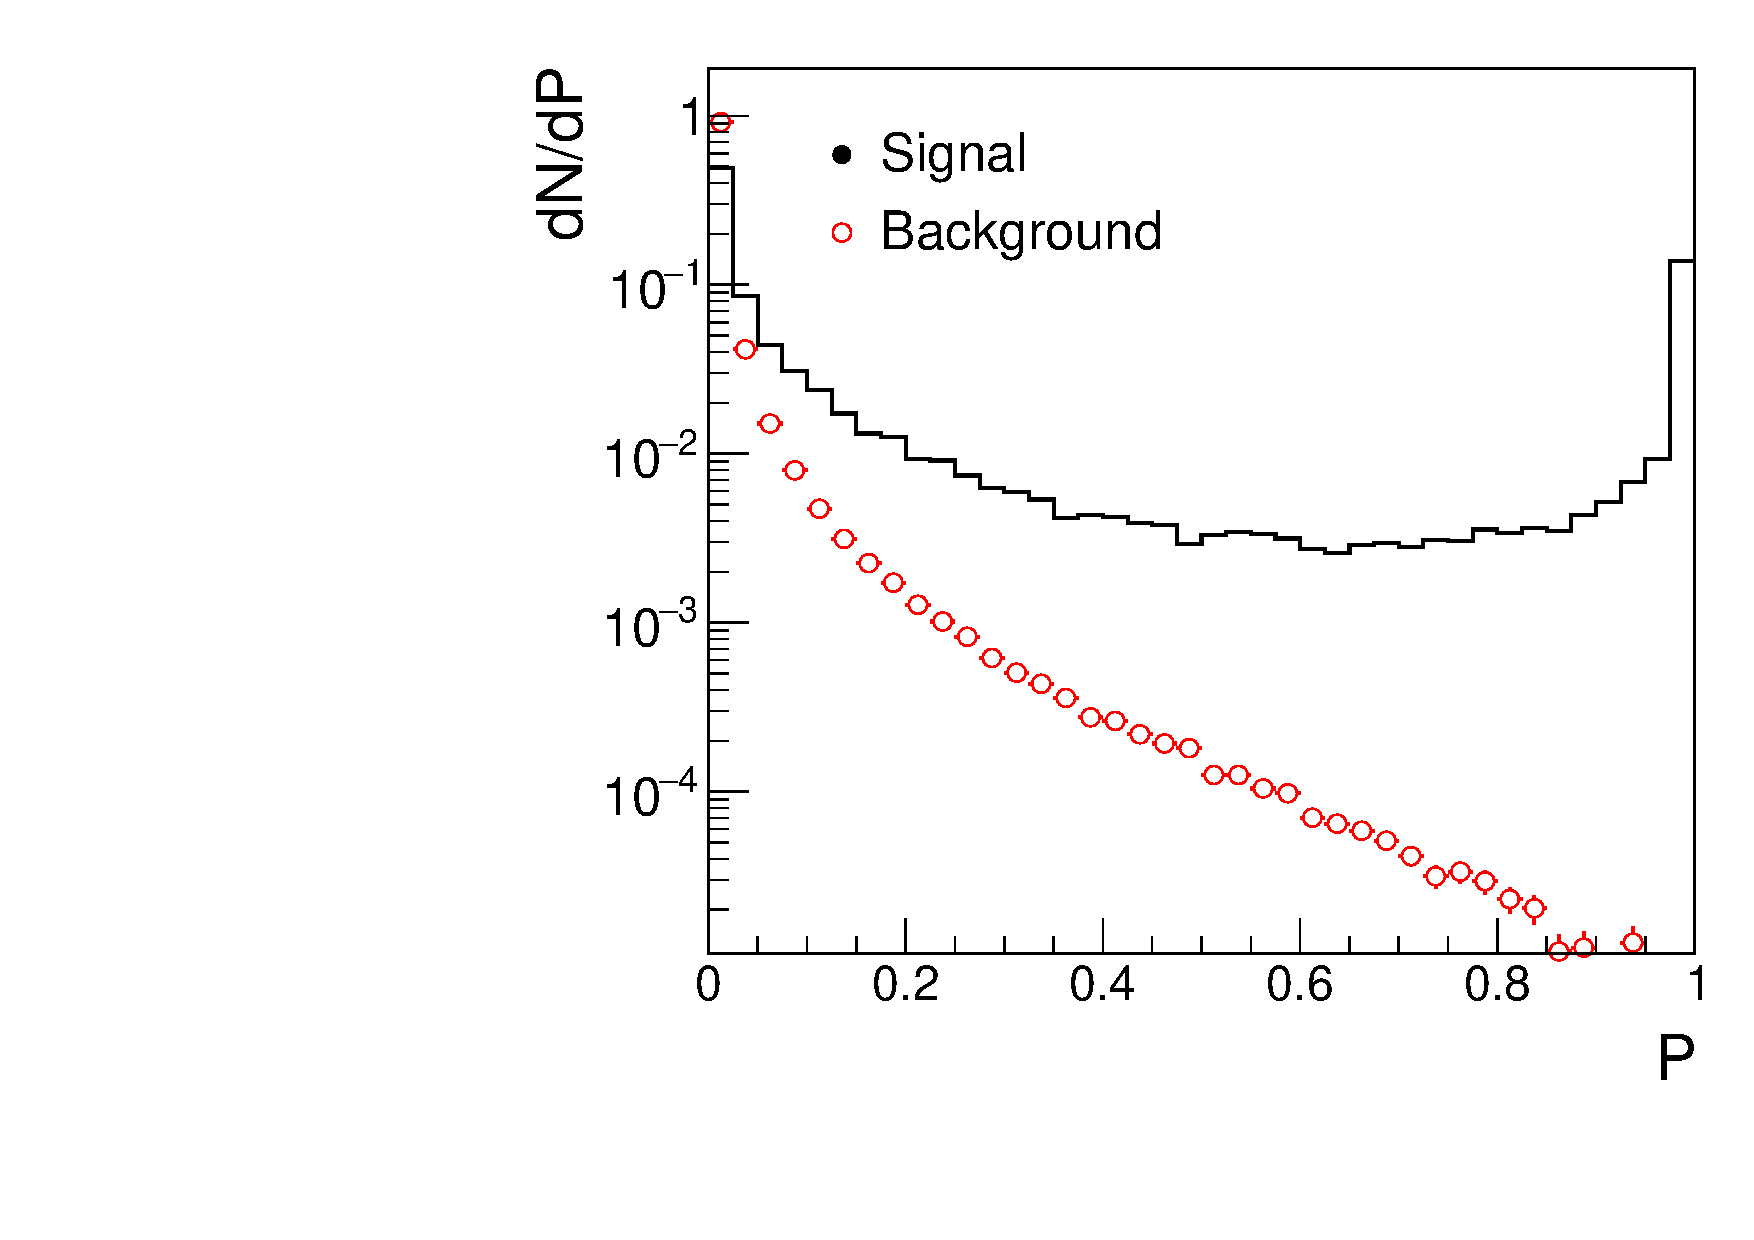
\includegraphics[width=0.48\textwidth]{plots/effectOfFakes_memLR_missingBJet.pdf}
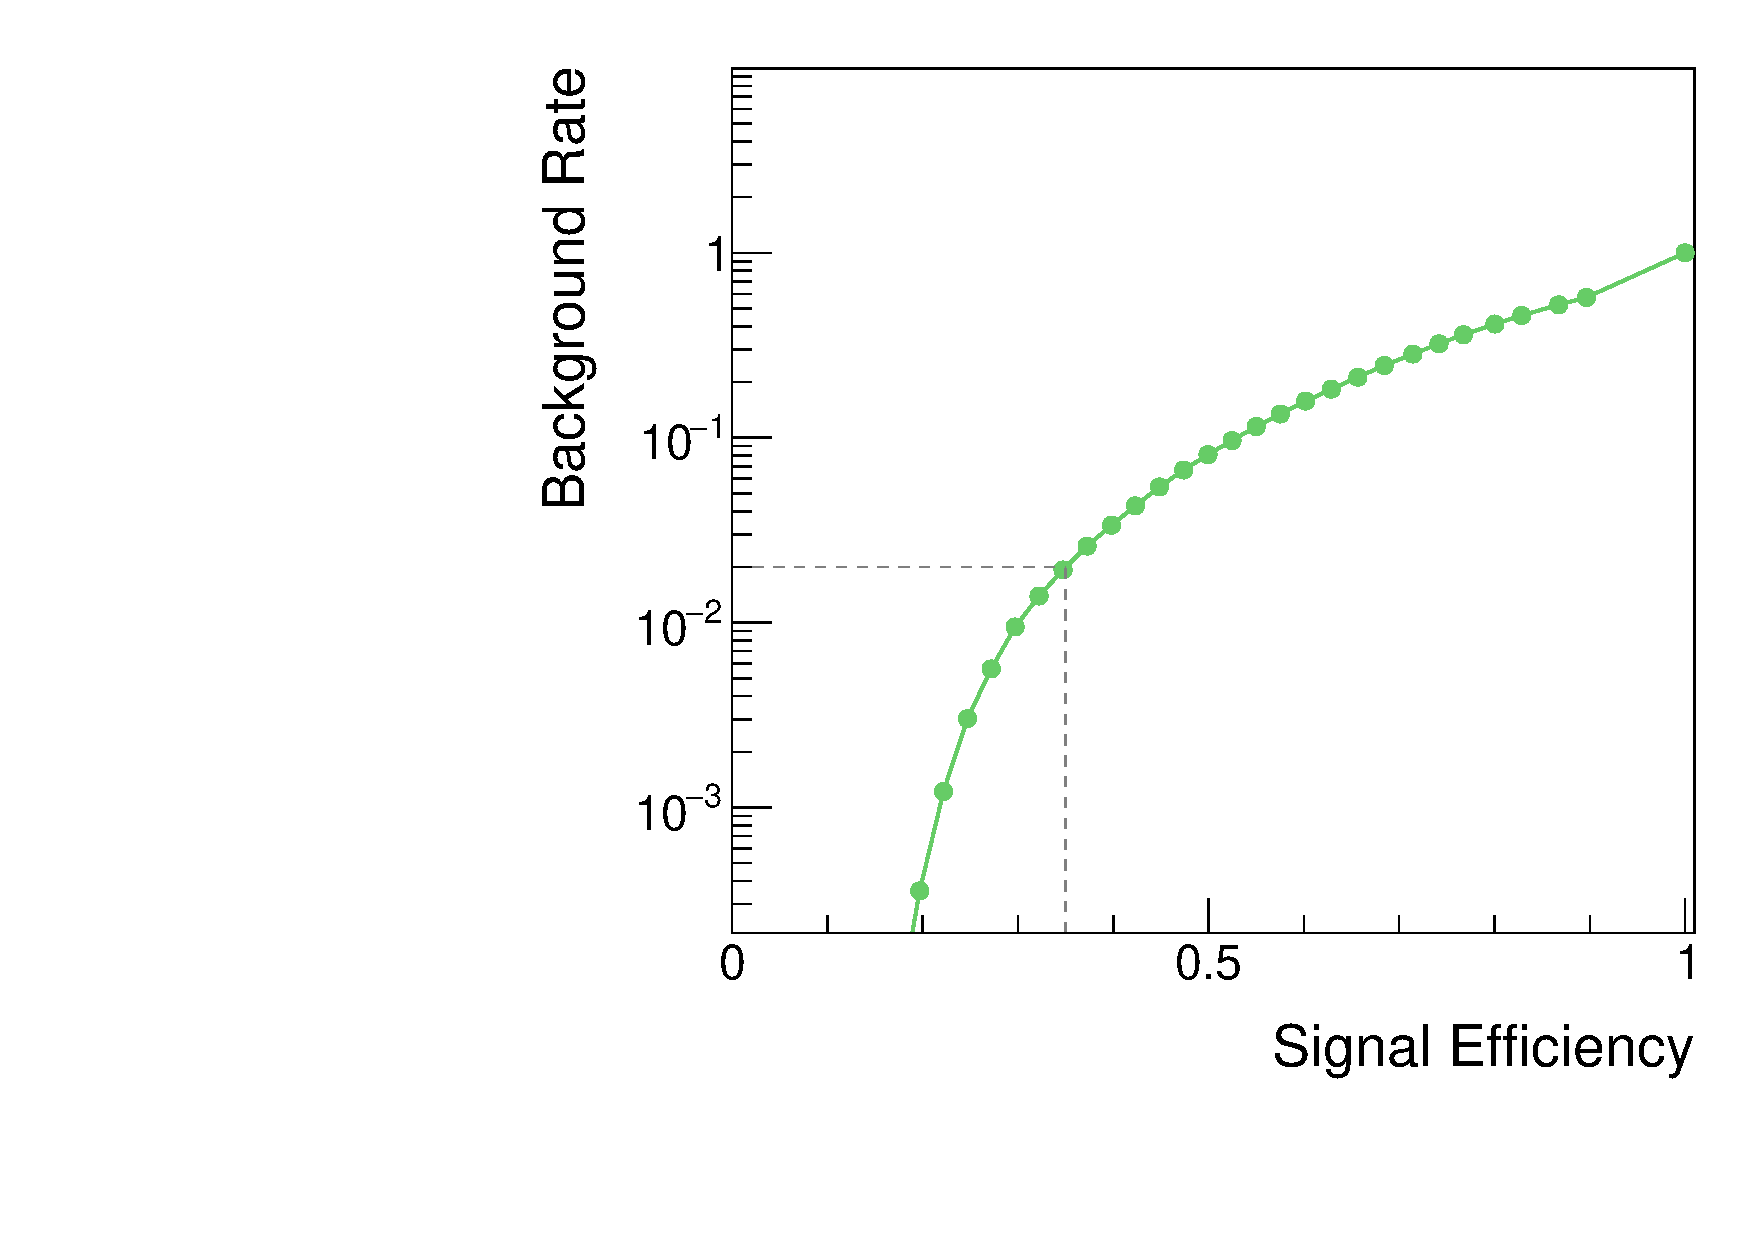
\includegraphics[width=0.48\textwidth]{plots/effectOfFakes_ROC_missingBJet.pdf}
\fi
\caption{
  Left: Distribution in the marginalized LR $P_{\textrm{m}}(\vecy)$, obtained for $\dihiggs$ signal and for $\ttbar$ background events.
  Right: Graph of background rate versus signal efficiency (``ROC curve''), obtained by applying a cut on the distribution shown on the left
  and varying the cut threshold.
}
\label{fig:memLR_and_ROC_missingBJet}
\end{figure}

Different options exist for using the marginalized LR $P_{\textrm{m}}(\vecy)$ in data analyses of $\dihiggs$ production at the LHC.
For instance, one may use the un-marginalized LR $P(\vecy)$ for events in which both reconstructed $\Pbottom$-jets pass tight $\Pbottom$-tagging criteria
and the marginalized LR $P_{\textrm{m}}(\vecy)$ for events in which one of the $\Pbottom$-jet candidate passes tight $\Pbottom$-tagging criteria,
while the other $\Pbottom$-jet candidate passes only loose $\Pbottom$-tagging criteria.
Alternatively, one may use the two-dimensional distribution in $P_{\textrm{m}}(\vecy)$ versus $P(\vecy)$ to separate the $\dihiggs$ signal from the $\ttbar$ background.
Yet another alternative is to use both likelihood ratios, $P_{\textrm{m}}(\vecy)$ and $P(\vecy)$,
as input to a machine-learning (ML) algorithm, for example a boosted decision tree~\cite{BDT} or an artificial neural network~\cite{ANN,chollet2015keras},
together with the $\Pbottom$-tagging discriminants of the two reconstructed $\Pbottom$-jet candidates and possibly other observables,
such as the total number of jets, the $\pT$ of the hadronic recoil, etc.
The CMS analysis of the associated production of a $\PHiggs$ boson with a top quark pair ($\Ptop\APtop\PHiggs$),
performed in the decay channel $\PHiggs \to \Pbottom\APbottom$ with the LHC Run $2$ data,
found that using the LR $P_{\textrm{m}}(\vecy)$ computed by the MEM as input to an ML algorithm
improved the signal-to-background separation compared to the case of either using the same ML algorithm without the LR $P_{\textrm{m}}(\vecy)$ as input
or of using the LR $P_{\textrm{m}}(\vecy)$ for the signal-to-background separation directly, without employing an ML algorithm~\cite{Sirunyan:2018mvw}.
The approach of using the LR $P_{\textrm{m}}(\vecy)$ as an input to an ML algorithm has the additional benefit
that other, subdominant, backgrounds can be included in the training of the ML algorithm, thereby further improving the sensitivity of the analysis.


\subsection{Effect of leading-order matrix elements}

The performance achieved in separating the $\dihiggs$ signal from the $\ttbar$ background
for MC samples simulated at LO and at NLO accuracy is shown in Fig.~\ref{fig:memLR_LO_vs_NLO}.
The signal and background events are studied on MC-truth level, assuming an optimal experimental resolution,
and are selected by requiring that both $\Pbottom$-jets are genuine $\Pbottom$-jets.
The corresponding ROC curve is presented in Fig.~\ref{fig:ROC_LO_vs_NLO}.
The usage of LO ME causes a moderate loss in the separation of the $\dihiggs$ signal from the $\ttbar$ background,
amounting to a few percent loss in signal efficiency (for the same background rate).

\begin{figure}
\ifx\ver\verPreprint
\setlength{\unitlength}{1mm}
\begin{center}
\begin{picture}(160,78)(0,0)
\put(0.0, 0.0){\mbox{\includegraphics*[height=78mm]
 {plots/lo_vs_nlo_memLR_signal.pdf}}}
\put(81.0, 0.0){\mbox{\includegraphics*[height=78mm]
 {plots/lo_vs_nlo_memLR_background.pdf}}}
\end{picture}
\end{center}
\fi
\ifx\ver\verPAPER
\centering
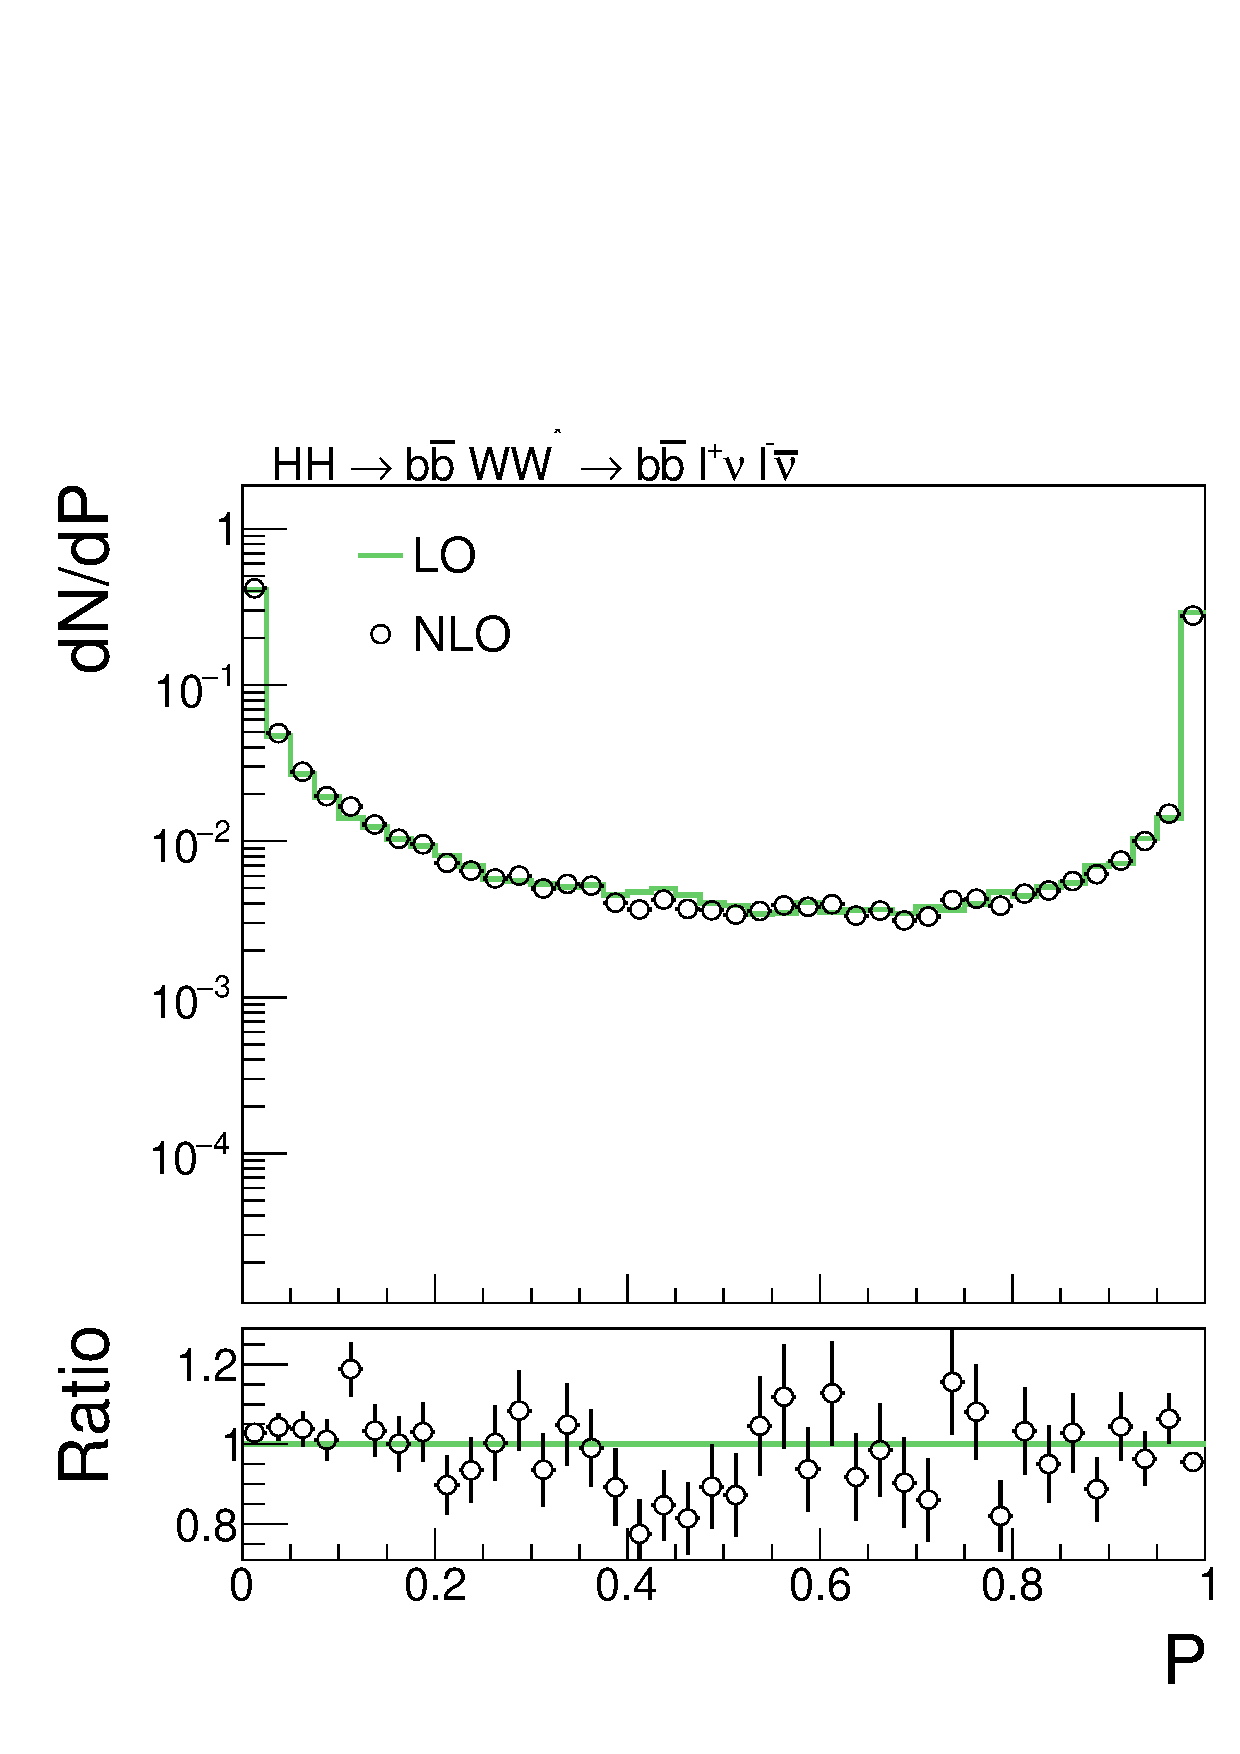
\includegraphics[width=0.48\textwidth]{plots/lo_vs_nlo_memLR_signal.pdf}
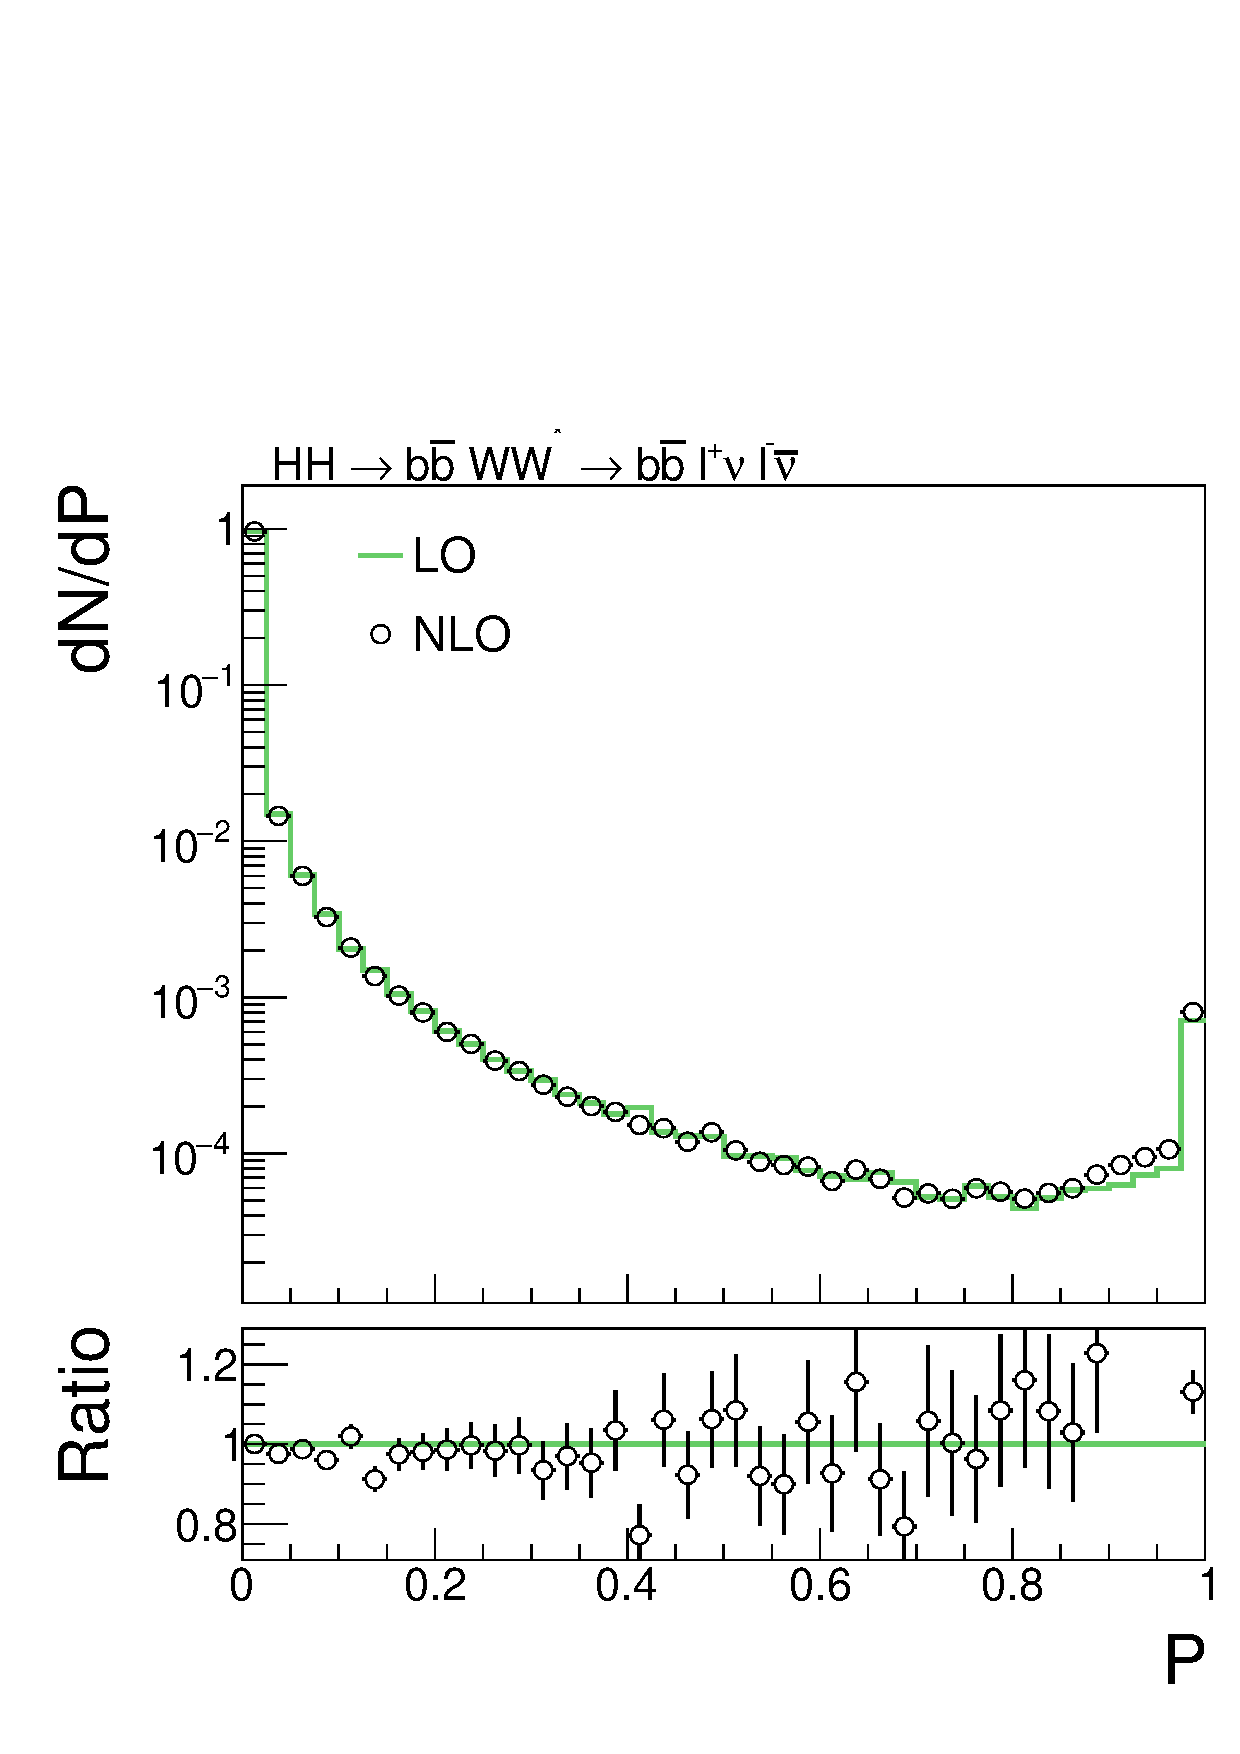
\includegraphics[width=0.48\textwidth]{plots/lo_vs_nlo_memLR_background.pdf}
\fi
\caption{
  Distribution in the LR $P(\vecy)$ 
  for $\dihiggs$ signal (left) and $\ttbar$ background (right) events
  simulated at LO and at NLO accuracy in pQCD.
  The signal and background events are studied on MC-truth level
  and are selected by requiring that both $\Pbottom$-jets are genuine $\Pbottom$-jets.
}
\label{fig:memLR_LO_vs_NLO}
\end{figure}

\begin{figure}
\ifx\ver\verPreprint
\setlength{\unitlength}{1mm}
\begin{center}
\begin{picture}(160,67)(0,0)
\put(39.5, 0.0){\mbox{\includegraphics*[height=67mm]
 {plots/lo_vs_nlo_ROC.pdf}}}
\end{picture}
\end{center}
\fi
\ifx\ver\verPAPER
\centering
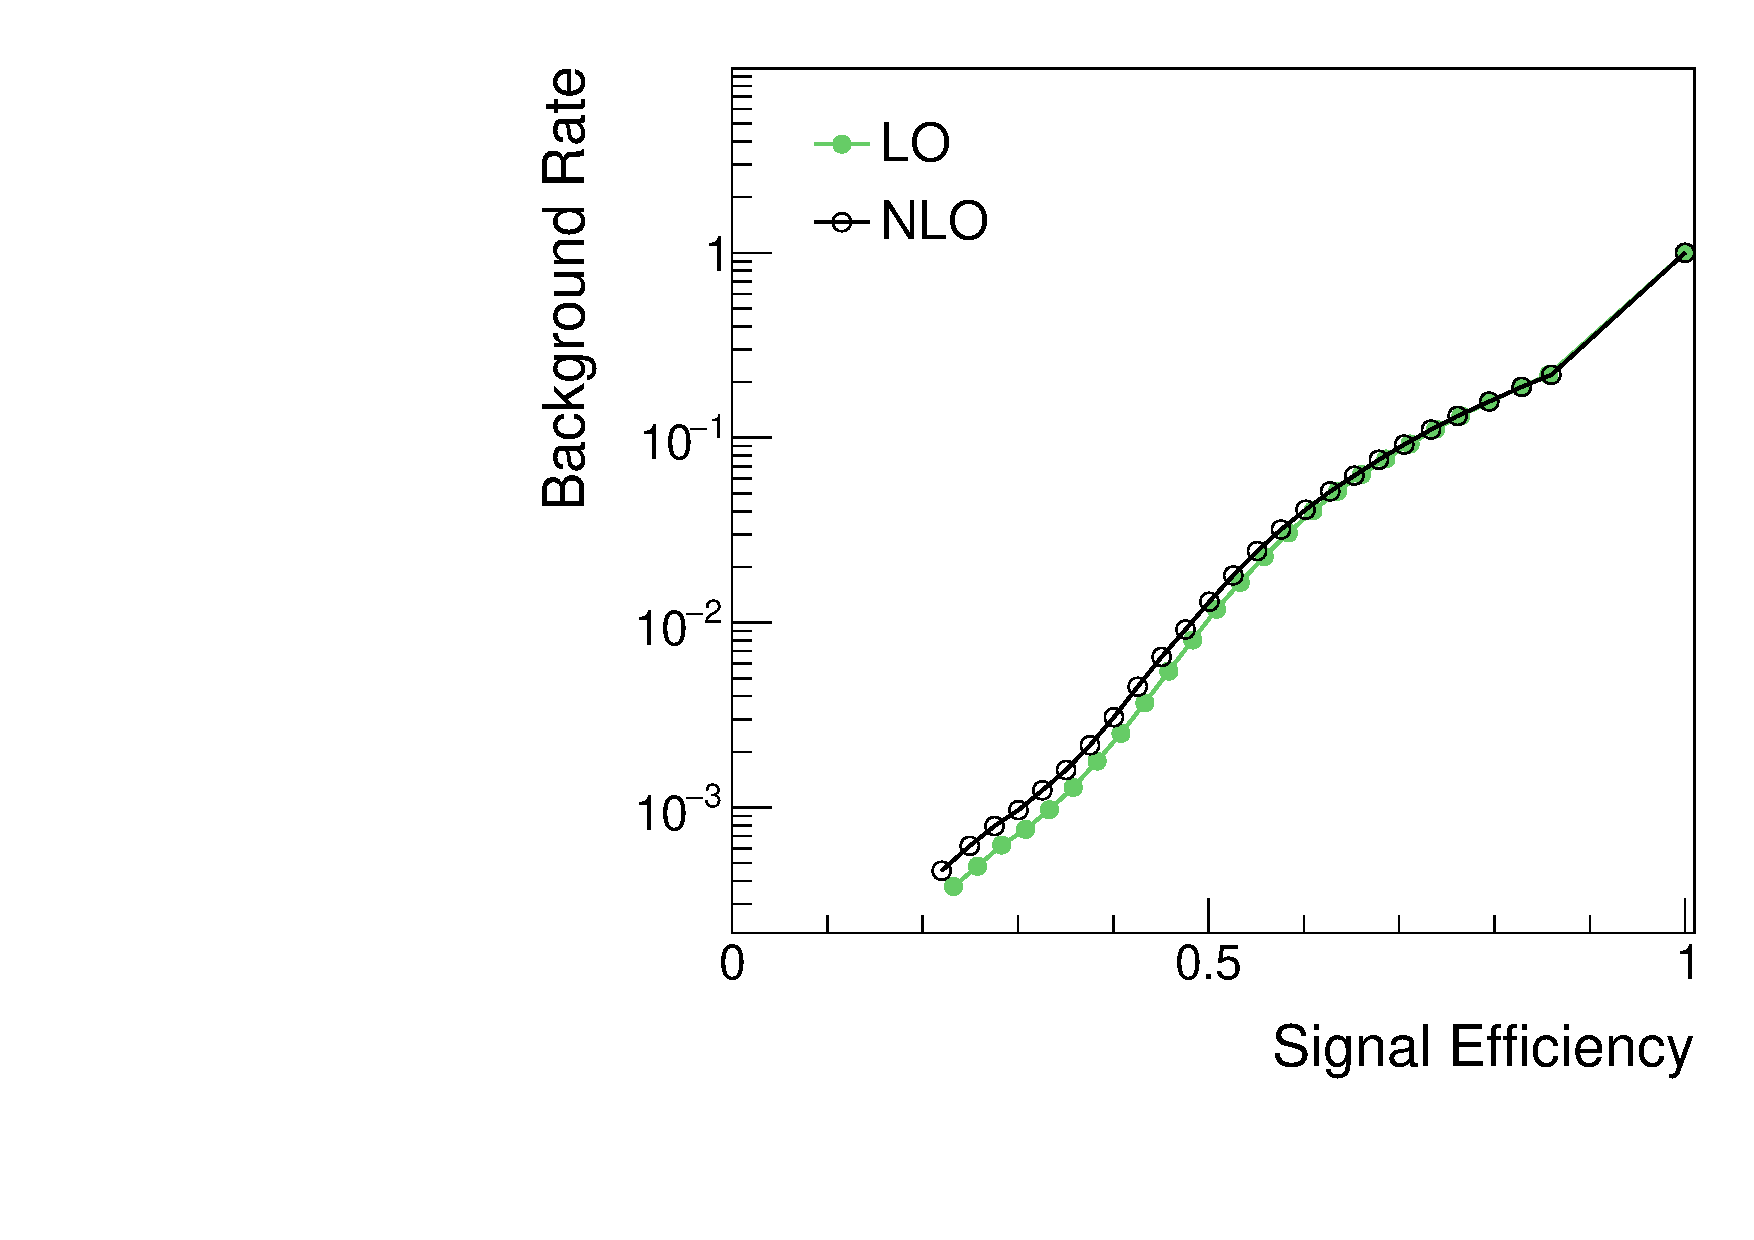
\includegraphics[width=0.48\textwidth]{plots/lo_vs_nlo_ROC.pdf}
\fi
\caption{
  Separation between the $\dihiggs$ signal and the $\ttbar$ background 
  for events simulated at LO and at NLO accuracy in pQCD.
  The signal and background events are studied on MC-truth level
  and are selected by requiring that both $\Pbottom$-jets are genuine $\Pbottom$-jets.
}
\label{fig:ROC_LO_vs_NLO}
\end{figure}


\subsection{Computing-time requirements of the MEM}
\label{sec:computing_time_requirements}

One remaining issue in practical applications of the MEM may be the computing time requirements.
Experimental analyses will usually need to evaluate the integrals given by Eqs.~(\ref{eq:mem_signal}) and~(\ref{eq:mem_background})
multiple times for each event in order to assess the effect of systematic uncertainties.
Taken together with the large cross section for $\ttbar$ production at the LHC,
the integrals in Eqs.~(\ref{eq:mem_signal}) and~(\ref{eq:mem_background}) may need to be computed in the order of $100$ million times.
Even with several thousands of computing jobs running in parallel,
as it is nowadays commonplace for experimental data analyses performed at the LHC,
the computation still requires a few weeks of nonstop computing time.
Several possibilities to speed up the numeric integrations, which take most of the computing time in practical applications of the MEM,
have been explored in the literature.
One alternative is to use vector integrands to evaluate the likelihood ratio for all systematic uncertainties simultaneously~\cite{CUBA},
taking advantage of the fact that the systematic uncertainties typically constitute small changes with respect to the nominal value.
Another alternative is to take advantage of the parallelizability of multidimensional integration and perform the integration on graphics processing units (GPUs).
Speedup factors of order $100$, compared to using a single core of a general-purpose central processing unit (CPU) 
such as the $2.30$~GHz Intel\TReg~Xeon\TReg~E5-2695V3 processor that we used for the studies presented in this paper,
are reported in the literature for performing numeric integrations on GPUs~\cite{Hagiwara:2009aq,Hagiwara:2009cy,Kanzaki:2010ym,Hagiwara:2013oka,Schouten:2014yza,Grasseau:2015vfa}.

\section{Summary}
\label{sec:summary}

We presented an application of the matrix element method 
to the search for non-resonant $\dihiggs$ production in the channel $\dihiggs \to \Pbottom\APbottom\PW\PW\virt$ at LHC,
focusing on events in which the two $\PW$ bosons decay to a pair of electrons or muons.
According to the Neyman-Pearson lemma,
the likelihood ratio $P(\vecy)$ given by Eq.~(\ref{eq:memLR}) provides the optimal separation of the $\dihiggs$ signal from the dominant irreducible $\ttbar$ background.
We have studied the separation of the $\dihiggs$ signal from the $\ttbar$ background at Monte-Carlo truth and at detector level.
The latter has been simulated using the $\textsc{DELPHES}$ fast-simulation framework.
For experimental conditions characteristic for the ATLAS and CMS experiments during LHC Run $2$,
we find that the $\ttbar$ background can be reduced to a level of $0.26\%$ for a signal efficiency of $35\%$.
We regard the potential of the matrix element method for enhancing the sensitivity of the analysis of $\dihiggs$ production in the channel $\dihiggs \to \Pbottom\APbottom\PW\PW\virt$
as promising and we hope this paper will motivate the ATLAS and CMS collaborations to employ the method in a full analysis.


\section*{Acknowledgements}

This work is supported by the Estonian Research Council grants IUT23-4 and PRG445.


\section{Appendix}
\label{sec:appendix}

In this section, we derive a few useful relations
that allow us to simplify the expression for the probability density $w_{i}(\vecy|\vecyhat)$ starting from Eq.~(\ref{eq:mem1}).
We begin by deriving relations for the TF of charged leptons and of $\Pbottom$-jets, which we present in Section~\ref{sec:appendix_TF}.
In Section~\ref{sec:appendix_mass_constraints}, 
we will derive relations corresponding to various mass constraints.
The constraints arise from the presence of BW propagators 
in the ME $\mathcal{M}_{i}(\vecyhat)$ for the signal ($i=0$) and for the background ($i=1$) hypothesis.
The effect of the BW propagators is that only those points $\vecphat$ in the $6$-particle phase space contribute to the value of the integral in Eq.~(\ref{eq:mem1})
for which certain systems of final state particles satisfy certain mass conditions.
The relations derived in Sections~\ref{sec:appendix_TF} and~\ref{sec:appendix_mass_constraints}
are used to transform Eq.~(\ref{eq:mem1}) 
into Eq.~(\ref{eq:mem_signal}) for the $\dihiggs$ signal hypothesis and 
into Eq.~(\ref{eq:mem_background}) for the $\ttbar$ background hypothesis, respectively.


\subsection{Relations for transfer functions}
\label{sec:appendix_TF}

We assume that the directions of electrons, muons, and $\Pbottom$-jets
as well as the energies of electrons and muons are measured with negligible experimental resolution.
Our assumption implies that the TF for electrons and muons is given by:
\begin{linenowrapper}
\begin{equation}
W_{\Plepton}(\vecp|\vecphat) = f(E,\theta,\phi) \, \delta(E - \Ehat) \cdot \delta(\theta - \thetahat) \cdot \delta(\phi - \phihat) \, ,
\label{eq:TF_ell}
\end{equation}
\end{linenowrapper}
while the TF for $\Pbottom$-jets is given by:
\begin{linenowrapper}
\begin{equation}
W(\vecp|\vecphat) = f(E,\theta,\phi) \, W(E|\Ehat) \, \delta(\theta - \thetahat) \cdot \delta(\phi - \phihat) \, ,
\label{eq:TF_b}
\end{equation}
\end{linenowrapper}
where $E$ denotes the energy, $\theta$ the polar angle, and $\phi$ the azimuthal angle of the electron, muon, or $\Pbottom$-jet.
The function $W(E|\Ehat)$ quantifies the experimental resolution with which the energy of $\Pbottom$-jets is measured.
We choose the function $W(E|\Ehat)$ such that it satisfies the following normalization condition:
\begin{linenowrapper}
\begin{equation*}
\int \, dE \, W(E|\Ehat) \equiv 1.
\end{equation*}
\end{linenowrapper}
The function $f(E,\theta,\phi)$ ensures that the TF satisfy the normalization condition 
\begin{linenowrapper}
\begin{equation*}
\int \, d^{3}\vecp \, \Omega(\vecp) \, W(\vecp|\vecphat) = 1 \, .
\end{equation*}
\end{linenowrapper}
We only consider those events, which pass the event selection criteria, \ie for which $\Omega(\vecp)$ is equal to one.
With $d^{3}\vecp = \beta \, E^{2} \, \sin\theta \, dE \, d\theta \, d\phi$, it follows that:
\begin{linenowrapper}
\begin{equation*}
1 \equiv \int \, dE \, d\theta \, d\phi \, \beta \, E^{2} \, \sin\theta \, f(E, \theta, \phi) \, W(E|\Ehat) \, \delta(\theta - \thetahat) \cdot \delta(\phi - \phihat) \, ,
\end{equation*}
\end{linenowrapper}
which implies:
\begin{linenowrapper}
\begin{equation}
f(E,\theta,\phi) = \frac{1}{\beta \, E^{2} \, \sin\theta} \, .
\label{eq:TF_f}
\end{equation}
\end{linenowrapper}
Eq.~(\ref{eq:TF_f}) holds for electrons and muons as well as for $\Pbottom$-jets.


\subsection{Relations for mass constraints}
\label{sec:appendix_mass_constraints}

As explained in Section~\ref{sec:mem},
the presence of BW propagators in the ME $\mathcal{M}_{i}(\vecphat)$ renders the numeric integration inefficient,
unless the numeric integration is restricted to those narrow slices in the $6$-particle PS where the mass constraints are satisfied.
We achieve the desired restriction by inserting suitable $\delta$-functions into the integrand on the RHS of Eq.~(\ref{eq:mem3}).
In order to avoid that the insertion of the $\delta$-functions changes the value of the integral,
we formally insert a factor of $1$, which we write as:
\begin{linenowrapper}
\begin{eqnarray}
1 \equiv \textrm{BW} \, \cdot \, \textrm{BW}^{-1} 
 & = & \frac{\pi}{m_{\X} \, \Gamma_{\X}} \, \delta( E_{\X}^{2} - |\vecp_{\X}|^{2} - m_{\X}^{2} ) \cdot 
\left( (E_{\X}^{2} - |\vecp_{\X}|^{2} - m_{\X}^{2})^{2} + (m_{\X} \, \Gamma_{\X})^{2} \right) \nonumber \\
 & = & \pi \, m_{\X} \, \Gamma_{\X} \, \delta( E_{\X}^{2} - |\vecp_{\X}|^{2} - m_{\X}^{2} ) \, ,
\label{eq:deltaFunc}
\end{eqnarray}
\end{linenowrapper}
where we have used the narrow-width approximation to replace the first $\textrm{BW}$ propagator by a $\delta$-function.
The symbol $\X$ in Eq.~(\ref{eq:deltaFunc}) refers to the on-shell particle, of mass $m_{\X}$ and width $\Gamma_{\X}$, which imposes the mass constraint.

We insert Eq.~(\ref{eq:deltaFunc}) into the integrand on the RHS of Eq.~(\ref{eq:mem3})
and then use the $\delta$-function $\delta( E_{\X}^{2} - |\vecp_{\X}|^{2} - m_{\X}^{2} )$ 
to eliminate the integration over $\Ehat$ for one of the daughter particles that the particle $\X$ decays into.
The $\delta$-function rule:
\begin{linenowrapper}
\begin{equation} 
\delta\left( g(x) \right) = \frac{1}{|g^{\prime}(x_{0})|} \, \delta( x - x_{0} ) 
\label{eq:deltaFuncRule}
\end{equation}
\end{linenowrapper}
yields a factor of $|g^{\prime}(x_{0})|^{-1} \defL \left\lvert \frac{\partial g}{\partial x} \right\rvert_{x = x_{0}}$,
which we account for when eliminating the integration over $\Ehat$.
The symbol $x_{0}$ denotes the root of $g(x)$. 


\subsubsection{Energy of \texorpdfstring{$\APbottom$}{bbar} produced in \texorpdfstring{$\PHiggs \to \Pbottom\APbottom$}{H->bbar} decay}
\label{sec:appendix_bEn_Hbb}

The condition that the mass of the $2$-particle system of $\Pbottom$ plus $\APbottom$ quark equals $m_{\PHiggs}$ implies that:
\begin{linenowrapper}
\begin{eqnarray}
m_{\PHiggs}^{2} \equiv m_{\Pbottom\APbottom}^{2} 
 & = & ( \Ehat_{\Pbottom} + \Ehat_{\APbottom} )^{2} - ( \vecphat_{\Pbottom} + \vecphat_{\APbottom} )^{2} \nonumber \\
 & = & \Ehat_{\Pbottom}^{2} + \Ehat_{\APbottom}^{2} + 2 \, \Ehat_{\Pbottom} \, \Ehat_{\APbottom} 
- |\vecphat_{\Pbottom}|^{2} - |\vecphat_{\APbottom}|^{2} - 2 \, \vecphat_{\Pbottom} \cdot \vecphat_{\APbottom} \nonumber \\
 & = & \underbrace{\Ehat_{\Pbottom}^{2} - |\vecphat_{\Pbottom}|^{2}}_{= m_{\Pbottom}^{2}} 
+ \underbrace{\Ehat_{\APbottom}^{2} - |\vecphat_{\APbottom}|^{2}}_{= m_{\Pbottom}^{2}} 
+ 2 \, \underbrace{\Ehat_{\Pbottom}}_{\defL a} \, \Ehat_{\APbottom} 
- 2 \, \underbrace{\sqrt{\Ehat_{\Pbottom}^{2} - m_{\Pbottom}^{2}} \, \vecehat_{\Pbottom} \cdot \vecehat_{\APbottom}}_{\defL b} \, 
 \sqrt{\Ehat_{\APbottom}^{2} - m_{\Pbottom}^{2}} \nonumber \\
\Longrightarrow 0 
 & = & \underbrace{\frac{m_{\PHiggs}^{2}}{2} - m_{\Pbottom}^{2}}_{\defL \Delta_{m_{\PHiggs}}} - a \, \Ehat_{\APbottom} + b \, \sqrt{\Ehat_{\APbottom}^{2} - m_{\Pbottom}^{2}} 
  \defR g(\Ehat_{\APbottom}) \, ,
\label{eq:bEn_Hbb1}
\end{eqnarray}
\end{linenowrapper}
where the symbol $\vecehat_{\Pbottom}$ denotes a unit vector in direction of the $\Pbottom$ quark
and the symbol $\APbottom$ a unit vector in direction of the $\APbottom$ quark.
Eq.~(\ref{eq:bEn_Hbb1}) has two solutions:
\begin{equation}
\Ehat_{\APbottom} = \frac{a \, \Delta_{m_{\PHiggs}} \pm |b| \, \sqrt{\Delta_{m_{\PHiggs}}^{2} - (a^{2} - b^{2}) \, m_{\Pbottom}^{2}}}{a^{2} - b^{2}} \, .
\label{eq:bEn_Hbb2}
\end{equation}
%Our solutions for $\Ehat_{\APbottom}$, given by Eq.~(\ref{eq:bEn_Hbb2}),
%are in agreement with the result given in Eq.~(56) of Ref.~\cite{CMS_AN_2013_313}.
%We believe there is a typo in the definition of $\Delta_{m_{\PHiggs}}$ in Section~A.2.3 of Ref.~\cite{CMS_AN_2013_313}.
%Following Ref.~\cite{CMS_AN_2013_313}, we discard the solution of lower energy and consider the solution of higher energy only, 
We discard the solution of lower energy and consider the solution of higher energy only, 
\ie we take the solution corresponding to the $+$ sign in Eq.~(\ref{eq:bEn_Hbb2}).

The derivative of the RHS of Eq.~(\ref{eq:bEn_Hbb1}) with respect to $\Ehat_{\APbottom}$ amounts to:
\begin{linenowrapper}
\begin{eqnarray}
\frac{1}{|g^{\prime}(\Ehat_{\APbottom})|} 
& = & \frac{1}{\Bigg\lvert a - \frac{b \, \Ehat_{\APbottom}}{\underbrace{\sqrt{\Ehat_{\APbottom}^{2} - m_{\Pbottom}^{2}}}_{= \beta_{\APbottom} \, \Ehat_{\APbottom}}} \Bigg\rvert}
 = \frac{1}{\left\lvert a - \frac{1}{\betahat_{\APbottom}} \, b \right\rvert} \nonumber \\
& = & \frac{1}{\left\lvert \Ehat_{\Pbottom} - \frac{1}{\betahat_{\APbottom}} \,
\smash{\underbrace{\sqrt{\Ehat_{\Pbottom}^{2} - m_{\Pbottom}^{2}}}_{= \betahat_{\Pbottom} \, \Ehat_{\Pbottom}}} \,
\smash{\underbrace{\vecehat_{\Pbottom} \cdot \vecehat_{\APbottom}}_{\defL \cos\sphericalangle(\vecehat_{\Pbottom},\vecehat_{\APbottom})}} \right\rvert}
 = \frac{1}{\left\lvert \Ehat_{\Pbottom} \, \left( 1 - \frac{\betahat_{\Pbottom}}{\betahat_{\APbottom}} \, \cos\sphericalangle(\vecehat_{\Pbottom},\vecehat_{\APbottom}) \right) \right\rvert} \, .
\label{eq:bEn_Hbb3}
\end{eqnarray}
\end{linenowrapper}

\vspace*{1em} % add a bit of vertical spacing

\subsubsection{Energy of \texorpdfstring{$\Pnu$}{v} produced in \texorpdfstring{$\PW \to \ellnu$}{W->lnu} decay}
\label{sec:appendix_nuEn_Wlnu}

The condition that the mass of the $2$-particle system of $\Plepton$ plus $\Pnu$ equals $m_{\PW}$ implies that:
\begin{linenowrapper}
\begin{eqnarray}
m_{\PW}^{2} \equiv m_{\Plepton\Pnu}^{2} 
 & = & ( \Ehat_{\Plepton} + \Ehat_{\Pnu} )^{2} - ( \vecphat_{\Plepton} + \vecphat_{\Pnu} )^{2} \nonumber \\
 & = & \Ehat_{\Plepton}^{2} + \Ehat_{\Pnu}^{2} + 2 \, \Ehat_{\Plepton} \, \Ehat_{\Pnu} 
- |\vecphat_{\Plepton}|^{2} - |\vecphat_{\Pnu}|^{2} - 2 \, \vecphat_{\Plepton} \cdot \vecphat_{\Pnu} \nonumber \\
 & = & \underbrace{\Ehat_{\Plepton}^{2} - |\vecphat_{\Plepton}|^{2}}_{= m_{\Plepton}^{2} \approx 0} 
+ \underbrace{\Ehat_{\Pnu}^{2} - |\vecphat_{\Pnu}|^{2}}_{= m_{\Pnu}^{2} \approx 0} 
+ 2 \, \Ehat_{\Plepton} \, \Ehat_{\Pnu} 
- 2 \, \underbrace{|\vecphat_{\Plepton}|}_{\approx \Ehat_{\Plepton}} \, \underbrace{|\vecphat_{\Pnu}|}_{\approx \Ehat_{\Pnu}} \, 
 \underbrace{\vecehat_{\Plepton} \cdot \vecehat_{\Pnu}}_{\defL \cos\sphericalangle(\vecehat_{\Plepton},\vecehat_{\Pnu})} \nonumber \\
 & = & 2 \, \Ehat_{\Plepton} \, \Ehat_{\Pnu} \, 
  \underbrace{\left(1 - \cos\sphericalangle(\vecehat_{\Plepton},\vecehat_{\Pnu})\right)}_{= 2 \, \sin^{2}\left(\frac{\sphericalangle(\vecehat_{\Plepton},\vecehat_{\Pnu})}{2}\right)} 
   = 4 \, \Ehat_{\Plepton} \, \Ehat_{\Pnu} \, \sin^{2}\left(\frac{\sphericalangle(\vecehat_{\Plepton},\vecehat_{\Pnu})}{2}\right) \nonumber \\
\Longrightarrow 0 & = & m_{\PW}^{2} - 4 \, \Ehat_{\Plepton} \, \Ehat_{\Pnu} \, \sin^{2}\left(\frac{\sphericalangle(\vecehat_{\Plepton},\vecehat_{\Pnu})}{2}\right)
  \defR g(\Ehat_{\Pnu}) \, ,
\label{eq:nuEn_Wlnu1}
\end{eqnarray}
\end{linenowrapper}
which has the solution:
\begin{equation}
\Ehat_{\Pnu} = \frac{m_{\PW}^{2}}{4 \, \Ehat_{\Plepton} \, \sin^{2}\left(\frac{\sphericalangle(\vecehat_{\Plepton},\vecehat_{\Pnu})}{2}\right)} \, .
\label{eq:nuEn_Wlnu2}
\end{equation}
The symbol $\sphericalangle(\vecehat_{\Plepton},\vecehat_{\Pnu})$ refers to the angle between the directions of the charged lepton and of the neutrino.
%Our result for $\Ehat_{\Pnu}$, given by Eq.~(\ref{eq:nuEn_Wlnu2}), is in agreement with the result given in Eq.~(54) of Ref.~\cite{CMS_AN_2013_313}.

The derivative of the RHS of Eq.~(\ref{eq:nuEn_Wlnu1}) with respect to $\Ehat_{\Pnu}$ yields:
\begin{linenowrapper}
\begin{equation}
\frac{1}{|g^{\prime}(\Ehat_{\Pnu})|} 
 = \frac{1}{4 \, \Ehat_{\Plepton} \, \sin^{2}\left(\frac{\sphericalangle(\vecehat_{\Plepton},\vecehat_{\Pnu})}{2}\right)} \, . 
\label{eq:nuEn_Wlnu3}
\end{equation}
\end{linenowrapper}

\subsubsection{Energy of \texorpdfstring{$\Pnu^{\ast}$}{v*} produced in \texorpdfstring{$\PHiggs \to \PW\PW^{\ast} \to \ellnu \, \ellnuStar$}{H->WW*->lvl*v*} decay}
\label{sec:appendix_nuEn_Hww}

As mentioned previously, we denote by $\Plepton^{\ast}$ and $\Pnu^{\ast}$ the charged lepton and the neutrino that originate from the decay of the off-shell $\PW$ boson.
The condition that the mass of the $4$-particle system of $\Plepton$, $\Pnu$, $\Plepton^{\ast}$, and $\Pnu^{\ast}$ equals $m_{\PHiggs}$ implies that:
\begin{linenowrapper}
\begin{eqnarray}
m_{\PHiggs}^{2} \equiv m_{\ellnuellnuStar}^{2} 
 & = & ( \underbrace{\Ehat_{\Plepton} + \Ehat_{\Pnu} + \Ehat_{\ellStar}}_{\defL \Ehat_{\ellnuellStar}} + \Ehat_{\nuStar} )^{2} 
- ( \underbrace{\vecphat_{\Plepton} + \vecphat_{\Pnu} + \vecphat_{\ellStar}}_{\defL \vecphat_{\ellnuellStar}} + \vecphat_{\nuStar} )^{2} \nonumber \\
 & = & \Ehat_{\ellnuellStar}^{2} + \Ehat_{\nuStar}^{2} + 2 \, \Ehat_{\ellnuellStar} \, \Ehat_{\nuStar} 
- |\vecphat_{\ellnuellStar}|^{2} - |\vecphat_{\nuStar}|^{2} - 2 \, \vecphat_{\ellnuellStar} \cdot \vecphat_{\nuStar} \nonumber \\
 & = & \underbrace{\Ehat_{\ellnuellStar}^{2} - |\vecphat_{\ellnuellStar}|^{2}}_{\defL m_{\ellnuellStar}^{2}} 
+ \underbrace{\Ehat_{\nuStar}^{2} - |\vecphat_{\nuStar}|^{2}}_{= m_{\Pnu}^{2} \approx 0} 
+ 2 \, \underbrace{\Ehat_{\ellnuellStar}}_{\defL a} \, \Ehat_{\nuStar} \nonumber \\
 & & \quad - 2 \, \underbrace{\sqrt{\Ehat_{\ellnuellStar}^{2} - m_{\ellnuellStar}^{2}} \, \vecehat_{\ellnuellStar} \cdot \vecehat_{\nuStar}}_{\defL b} \, 
 \underbrace{|\vecphat_{\nuStar}|}_{\approx \Ehat_{\nuStar}} \nonumber \\
 & = & m_{\ellnuellStar}^{2} + 2 \, a \, \Ehat_{\nuStar} - 2 \, b \, \Ehat_{\nuStar} \nonumber \\
\Longrightarrow 0 & = & \underbrace{\frac{m_{\PHiggs}^{2} - m_{\ellnuellStar}^{2}}{2}}_{\defL \Delta_{m_{\PHiggs}}} - a \, \Ehat_{\nuStar} + b \, \Ehat_{\nuStar}
  \defR g(\Ehat_{\nuStar}) \, ,
\label{eq:nuEn_Hww1}
\end{eqnarray}
\end{linenowrapper}
which has the solution:
\begin{linenowrapper}
\begin{eqnarray}
\Ehat_{\nuStar}
 & = & \frac{\Delta_{m_{\PHiggs}}}{a - b} 
 = \frac{m_{\PHiggs}^{2} - m_{\ellnuellStar}^{2}}{2 \, \Big( \Ehat_{\ellnuellStar}
- \underbrace{\sqrt{\Ehat_{\ellnuellStar}^{2} - m_{\ellnuellStar}^{2}}}_{= \betahat_{\ellnuellStar} \, \Ehat_{\ellnuellStar}} \,
 \underbrace{\vecehat_{\ellnuellStar} \cdot \vecehat_{\nuStar}}_{\defL \cos\sphericalangle(\vecehat_{\ellnuellStar},\vecehat_{\nuStar})} \Big)} \nonumber \\
 & = & \frac{m_{\PHiggs}^{2} - m_{\ellnuellStar}^{2}}{2 \, \Ehat_{\ellnuellStar} \, 
\left( 1 - \betahat_{\ellnuellStar} \, \cos\sphericalangle(\vecehat_{\ellnuellStar},\vecehat_{\nuStar}) \right)} \, ,
\label{eq:nuEn_Hww2}
\end{eqnarray}
\end{linenowrapper}
where, for the purpose of shortening the nomenclature, we denote by the symbols $\Ehat_{\ellnuellStar}$ and $\vecphat_{\ellnuellStar}$ the energy and the momentum
of the $3$-particle system comprised of the neutrino originating from the decay of the on-shell $\PW$ boson and of the two charged leptons,
by $\vecehat_{\ellnuellStar}$ a unit vector in direction of $\vecphat_{\ellnuellStar}$,
and by $m_{\ellnuellStar}$ the mass of this $3$-particle system.

The derivative of the RHS of Eq.~(\ref{eq:nuEn_Hww1}) with respect to $\Ehat_{\nuStar}$ amounts to:
\begin{linenowrapper}
\begin{eqnarray}
\frac{1}{|g^{\prime}(\Ehat_{\nuStar})|} 
 & = &\frac{1}{|a - b|} 
  = \frac{1}{\Ehat_{\ellnuellStar} - \underbrace{\sqrt{\Ehat_{\ellnuellStar}^{2} - m_{\ellnuellStar}^{2}}}_{= \betahat_{\ellnuellStar} \, \Ehat_{\ellnuellStar}} \, 
\cos\sphericalangle(\vecehat_{\ellnuellStar},\vecehat_{\nuStar})} \nonumber \\
 & = & \frac{1}{\Ehat_{\ellnuellStar} \left( 1 - \betahat_{\ellnuellStar} \, \cos\sphericalangle(\vecehat_{\ellnuellStar},\vecehat_{\nuStar}) \right)} \, .
\label{eq:nuEn_Hww3}
\end{eqnarray}
\end{linenowrapper}

\subsubsection{Energy of \texorpdfstring{$\Pbottom$}{b}  (\texorpdfstring{$\APbottom$}{bbar}) produced in \texorpdfstring{$\Ptop \to \Pbottom\PW^{+} \to \Pbottom\ellPlusnu$}{t->bW+->bl+v} (\texorpdfstring{$\APtop \to \APbottom\PW^{-} \to \APbottom\ellMinusnu$}{tbar->bbarW- ->bbarl-vbar}) decay}
\label{sec:appendix_bEn_top}

The condition that the mass of of the $3$-particle system comprised of the $\Pbottom$ quark, the charged anti-lepton, and the neutrino equals $m_{\Ptop}$ implies that:
\begin{linenowrapper}
\begin{eqnarray}
m_{\Ptop}^{2} \equiv m_{\Pbottom\ellPlusnu}^{2} 
 & = & ( \Ehat_{\Pbottom} + \underbrace{\Ehat_{\ellPlus} + \Ehat_{\Pnu}}_{\defL \Ehat_{\ellPlusnu}} )^{2} 
- ( \vecphat_{\Pbottom} + \underbrace{\vecphat_{\ellPlus} + \vecphat_{\Pnu}}_{\defL \vecphat_{\ellPlusnu}} )^{2} \nonumber \\
 & = & \Ehat_{\Pbottom}^{2} + \Ehat_{\ellPlusnu}^{2} + 2 \, \Ehat_{\Pbottom} \, \Ehat_{\ellPlusnu} 
- |\vecphat_{\Pbottom}|^{2} - |\vecphat_{\ellPlusnu}|^{2} - 2 \, \vecphat_{\Pbottom} \cdot \vecphat_{\ellPlusnu} \nonumber \\
 & = & \underbrace{\Ehat_{\Pbottom}^{2} - |\vecphat_{\Pbottom}|^{2}}_{= m_{\Pbottom}^{2}} 
+ \underbrace{\Ehat_{\ellPlusnu}^{2} - |\vecphat_{\ellPlusnu}|^{2}}_{= m_{\PW}^{2}} 
+ 2 \, \underbrace{\Ehat_{\ellPlusnu}}_{\defL a} \, \Ehat_{\Pbottom} \nonumber \\
 & & \quad - 2 \, \underbrace{\sqrt{\Ehat_{\ellPlusnu}^{2} - m_{\PW}^{2}} \, \vecehat_{\ellPlusnu} \cdot \vecehat_{\Pbottom}}_{\defL b} \, 
 \sqrt{\Ehat_{\Pbottom}^{2} - m_{\Pbottom}^{2}} \nonumber \\
\Longrightarrow 0 & = & \underbrace{\frac{m_{\Ptop}^{2} - m_{\Pbottom}^{2} - m_{\PW}^{2}}{2}}_{\defL \Delta_{m_{\Ptop}}} - a \, \Ehat_{\Pbottom} + b \, \sqrt{\Ehat_{\Pbottom}^{2} - m_{\Pbottom}^{2}} 
  \defR g(\Ehat_{\Pbottom}) \, ,
\label{eq:bEn_top1}
\end{eqnarray}
\end{linenowrapper}
where we denote the energy of the system of the charged anti-lepton and of the neutrino by the symbol $\Ehat_{\ellPlusnu}$ 
and the momentum of this system by the symbol $\vecphat_{\ellPlusnu}$.
The symbol $\vecehat_{\ellPlusnu}$ denotes a unit vector in direction of $\vecphat_{\ellPlusnu}$.
The mass of this system equals $m_{\PW}$, as the $\PW$ boson produced in the decay $\Ptop \to \Pbottom\PW^{+}$ is on-shell.
Eq.~(\ref{eq:bEn_top1}) has two solutions:
\begin{linenowrapper}
\begin{equation}
\Ehat_{\Pbottom} = \frac{a \, \Delta_{m_{\Ptop}} \pm |b| \, \sqrt{\Delta_{m_{\Ptop}}^{2} - (a^{2} - b^{2}) \, m_{\Pbottom}^{2}}}{a^{2} - b^{2}} \, .
\label{eq:bEn_top2}
\end{equation}
\end{linenowrapper}
%The result for $\Ehat_{\Pbottom}$ is in agreement with the result given in Eq.~(55) of Ref.~\cite{CMS_AN_2013_313}.
%Following Ref.~\cite{CMS_AN_2013_313}, we discard the solution of lower energy and consider the solution of higher energy only, 
We discard the solution of lower energy and consider the solution of higher energy only,
\ie we take the solution corresponding to the $+$ sign in Eq.~(\ref{eq:bEn_top2}).

The derivative of the RHS of Eq.~(\ref{eq:bEn_top1}) with respect to $\Ehat_{\Pbottom}$ yields:
\begin{linenowrapper}
\begin{eqnarray}
\frac{1}{|g^{\prime}(\Ehat_{\Pbottom})|} 
 & = & \frac{1}{\Bigg\lvert a - \frac{b \, \Ehat_{\Pbottom}}{\underbrace{\sqrt{\Ehat_{\Pbottom}^{2} - m_{\Pbottom}^{2}}}_{= \beta_{\Pbottom} \, \Ehat_{\Pbottom}}} \Bigg\rvert}
  = \frac{1}{\left\lvert a - \frac{1}{\betahat_{\Pbottom}} \, b \right\rvert}
  = \frac{1}{\left\lvert \Ehat_{\ellPlusnu} - \frac{1}{\betahat_{\Pbottom}} \,
\smash{\underbrace{\sqrt{\Ehat_{\ellPlusnu}^{2} - m_{\PW}^{2}}}_{= \betahat_{\ellPlusnu} \, \Ehat_{\ellPlusnu}}} \,
\smash{\underbrace{\vecehat_{\ellPlusnu} \cdot \vecehat_{\Pbottom}}_{\defL \cos\sphericalangle(\vecehat_{\ellPlusnu},\vecehat_{\Pbottom})}} \right\rvert} \nonumber \\
 & = & \frac{1}{\left\lvert \Ehat_{\ellPlusnu} \, \left( 1 - \frac{\betahat_{\ellPlusnu}}{\betahat_{\Pbottom}} \, \cos\sphericalangle(\vecehat_{\ellPlusnu},\vecehat_{\Pbottom}) \right) \right\rvert} \, .
\label{eq:bEn_top3}
\end{eqnarray}
\end{linenowrapper}

The corresponding expressions for the case of $\APbottom$ quark, charged lepton, and anti-neutrino are identical to Eqs.~(\ref{eq:bEn_top2}) and~(\ref{eq:bEn_top3}),
except that the symbol $\Pbottom$ is replaced by $\APbottom$ and the symbols $\ellPlus$ and $\Pnu$ are replaced by $\ellMinus$ and $\APnu$.


\section*{References}
\bibliography{bbwwMEM}
%\endgroup

\end{document}
